\documentclass[times, utf8, zavrsni, numeric]{fer}
\usepackage{booktabs}
\usepackage{pdfpages}
\usepackage{graphicx}
\usepackage{float}
\usepackage{listings}
\usepackage[bottom]{footmisc}
%\def\verbatim@font{\linespread{1}\normalfont\ttfamily}
\usepackage{multirow}
\usepackage{caption}
\usepackage{subcaption}
\nocite{*}

\begin{document}

% TODO: Navedite broj rada.
\thesisnumber{456}

% TODO: Navedite naslov rada.
\title{Prilagodba korisničkih sučelja web-aplikacija konceptima pokretnog dizajna}

% TODO: Navedite vaše ime i prezime.
\author{Sara Tedeško}

\maketitle

% Ispis stranice s napomenom o umetanju izvornika rada. Uklonite naredbu \izvornik ako želite izbaciti tu stranicu.
%\izvornik
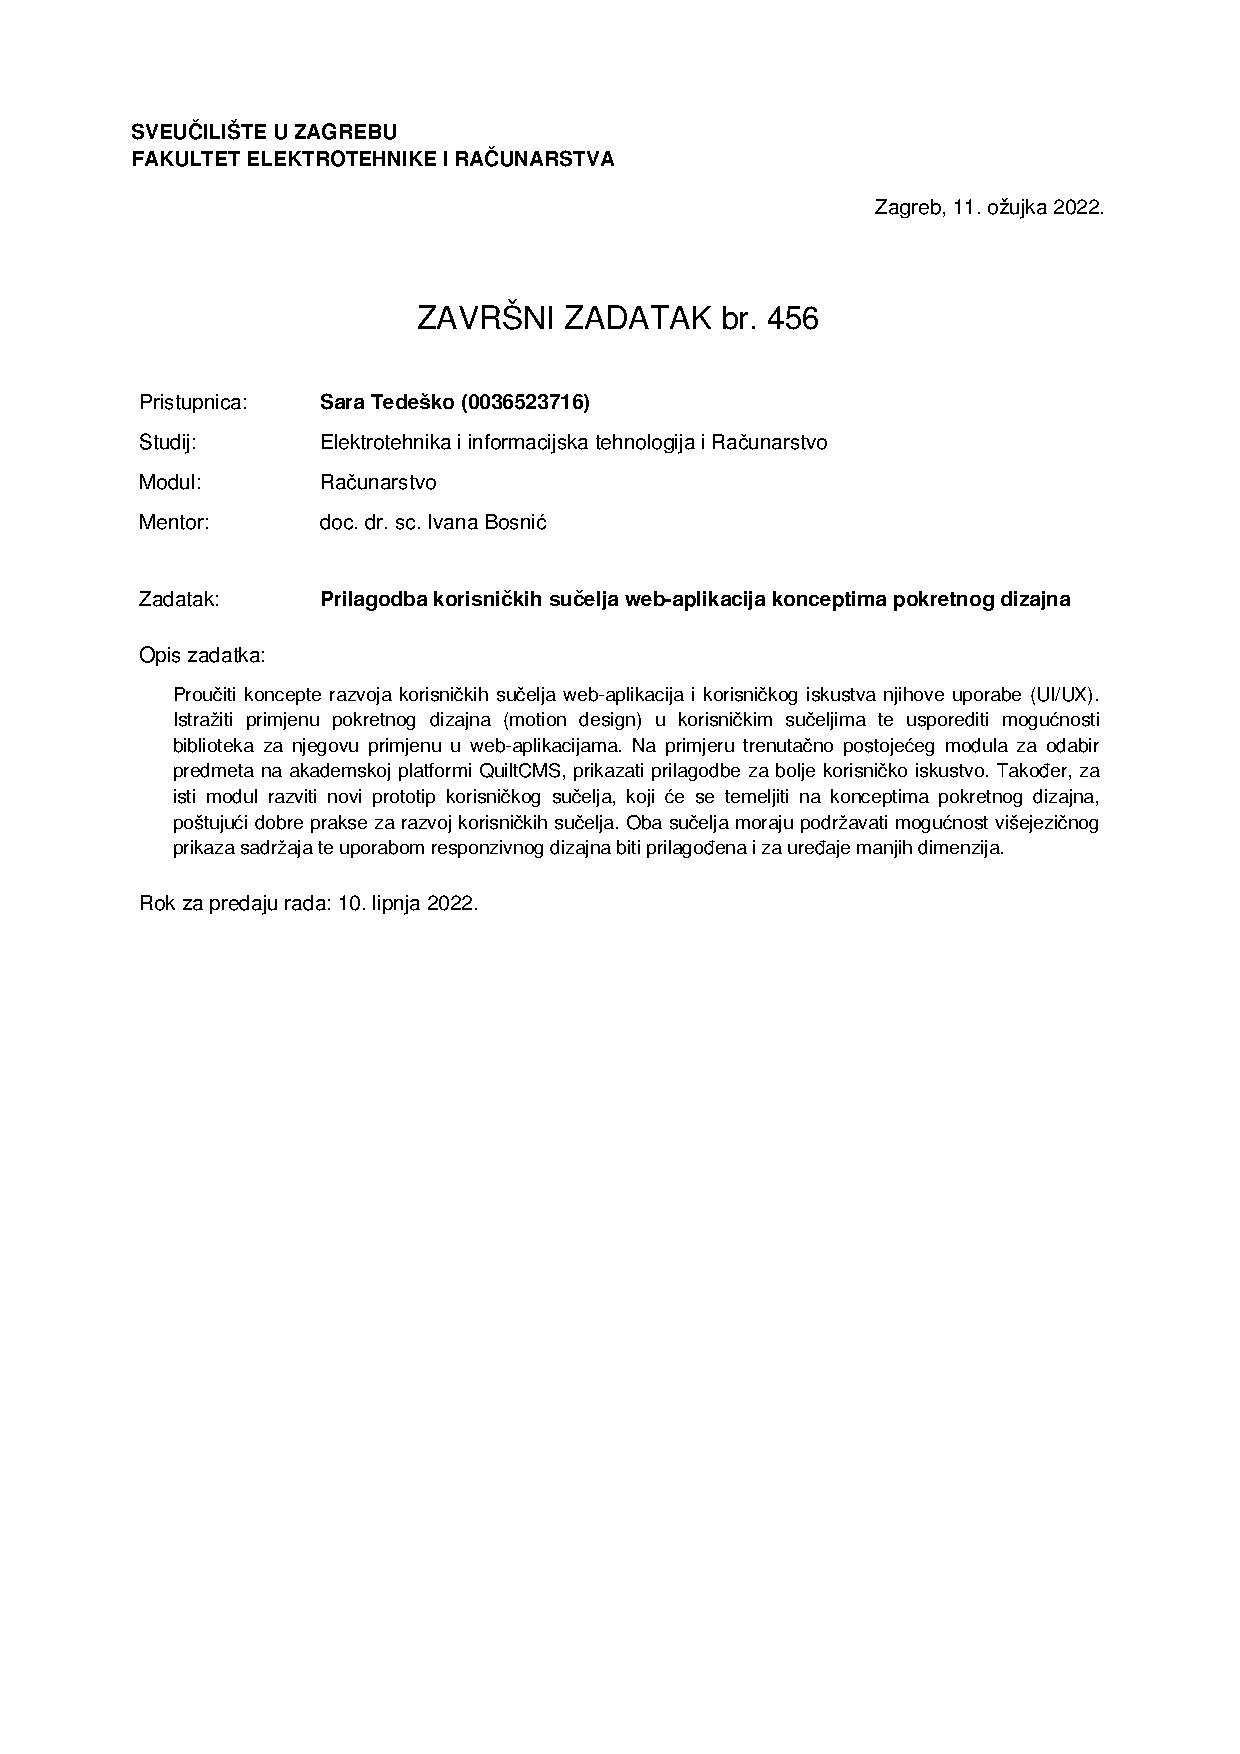
\includepdf[pages=-]{izvornik.pdf}

% Dodavanje zahvale ili prazne stranice. Ako ne želite dodati zahvalu, naredbu ostavite radi prazne stranice.
\noindent\zahvala{Zahvaljujem mentorici doc. dr. sc. Ivani Bosnić i mr. sc. Siniši Tomiću na stručnom vodstvu te prijateljima Teni Đuretek, Franu Markulinu i Martini Ludban na emotivnoj potpori pri izradi ovoga rada.}

\tableofcontents

\chapter{Uvod}
Mnoge web-stranice, sučelja i aplikacije nisu rađene s idejom korisnika na prvom mjestu. Drugim riječima, nisu pristupačne većem broju korisnika ciljane skupine ili su nejasne i neintuitivne za korištenje. \textbf{Uporabljivost} (\textit{usability}) weba stupanj je \textbf{jednostavnosti korištenja} web-stranice. To je mjera koliko dobro korisnik može koristiti proizvod za postizanje definiranog cilja na \textbf{učinkovit i zadovoljavajuć način} \cite{usability}. Definicija uporabljivosti prema normi ISO 9241-11 je „mjera u kojoj korisnici određene skupine mogu uporabiti proizvod kako bi postigli zadane ciljeve učinkovito, djelotvorno i sa zadovoljstvom u zadanom kontekstu uporabe.“ \cite{citat} Web-stranica s dobrom uporabljivosti je ona koja korisnicima omogućuje \textbf{jednostavnu, intuitivnu i ugodnu interakciju} \cite{usability2}.


Cilj ovog rada je poboljšati dizajn trenutačno postojećeg sučelja za upis godine na Fakultetu elektrotehnike i računarstva koji bi bio više usmjeren na \textbf{korisničko iskustvo} (\textit{user experience - UX}) i imao implementirani \textbf{pokretni dizajn} (\textit{motion design}) ondje gdje je koristan. Osim toga potrebno je osmisliti drugačiji dizajn aplikacije poštujući iste principe.


U drugom poglavlju objašnjena je teorijska pozadina za korisničko iskustvo i pokretni dizajn. Objašnjene su dobre prakse i principi za izradu web-sučelja imajući na umu uporabljivost i \textbf{pristupačnost} (\textit{accessability}) što većem broju korisnika.


U trećem poglavlju opisan je postojeći modul. Nakon opisa starog dizajna nalazi se potpoglavlje u kojem je evaluiran trenutačni dizajn te nakon toga predstavljen opis provedenih promjena na postojećem modulu i poboljšani dizajn. Na promijenjenom dizajnu također je provedena je kratka evaluacija.


U četvrtom poglavlju opisan je novi prototip aplikacije, odnosno drugačiji dizajn. Opisan je njezin izgled i prednosti koje ovakav izgled ima na korisničko iskustvo. I nad ovom verzijom aplikacije obavljena je evaluacija čiji se rezultati nalaze u potpoglavlju petog poglavlja.

U petom poglavlju spomenute su u radu korištene tehnologije te usporedba različitih biblioteka korištenih za implementaciju pokretnog dizajna.

U šestom poglavlju provedena je usporedba sva tri dizajna. Navedene su i slikama prikazane razlike između starog, poboljšanog i novog dizajna. Opisane su bitne promjene i uspoređene prosječne ocjene iskustva korištenja aplikacija u evaluacijama studenata.



\chapter{Načela dobre izrade korisničkog sučelja}
    \section{Korisničko sučelje i korisničko iskustvo}
    \textbf{Korisničko sučelje} (\textit{user interface - UI}) niz je ekrana, stranica i vizualnih elemenata poput gumba i ikona koji omogućuju osobi interakciju s proizvodom \cite{uivsux}. To je vizualni identitet i konačan \textbf{izgled} korisničkog sučelja. Dizajn proizvoda je dio procesa izrade dobrog korisničkog iskustva
    
    
    Dizajn \textbf{korisničkog iskustva} je dizajn koji se zasniva na \textbf{iskustvu} korisnika prilikom korištenja aplikacije \cite{pristup}. To je proces planiranja iskustva koje osoba ima kada stupi u interakciju s proizvodom \cite{uxui}. Kroz planiranje, korisniku se pokušavaju pružiti smislena i intuitivna rješenja. Taj proces uključuje \textbf{istraživanje, dizajn i evaluacija} proizvoda \cite{a11y}. Postavljamo \textbf{cilj i svrhu} našeg proizvoda. S obzirom na ciljanu skupinu koja će proizvod koristiti provodi se istraživanje. Nakon toga osmišljava se najbolji mogući \textbf{dizajn}. Za svaki osmišljeni dizajn mora se obaviti \textbf{evaluacija} prije objavljivanja proizvoda. Zlatni broj osoba za istraživanje i evaluaciji je pet jer se pomoću njih otkrije oko 90\% problema nekog proizvoda \cite{uxdesigner}. Dizajn korisničkog iskustva uzima u obzir svaki element koji oblikuje iskustvo, kako se korisnik osjeća i koliko je korisniku lako izvršiti željenu radnju. Cilj dizajna korisničkog iskustva je stvoriti \textbf{lako, učinkovito, jednostavno i ugodno iskustvo} za korisnika \cite{uivsux}.

    \section{Pokretni dizajn}
    Dobro korišten pokretni dizajn može uvelike doprinijeti korisničkom iskustvu. U korisničkom iskustvu, animacije mogu biti \textbf{korisne i komunikativne}, ako se ne koriste prečesto. Pokret je najčešće prikladan kao oblik suptilne povratne informacije za mikrointerakcije.
    
    Velika prednost, ali i nedostatak pokretnog dizajna je to što \textbf{privlači pozornost} korisnika i zaokupljuje ga. Perifernim vidom možemo detektirati kretanje izvan središta našeg vidnog polja, što znači da smo osjetljivi i skloni da nas ometa bilo koja vrsta pokreta (značajna ili ne). Zbog toga pokret u korisničkim sučeljima može lako postati dosadan ili naporan. Teško ga je prestati opažati, a ako nije važno za željeni zadatak, može značajno pogoršati korisničko iskustvo. S jedne strane, suptilni pokazatelj može se učiniti prirodnim i korisnik često ostaje nesvjestan da je uopće ondje, ali s druge strane, nepotrebne animacije ometaju korisnika. Nadalje, korištenje animacije za otimanje pažnje korisnika ili stvaranje straha od gubitka neetička je primjena principa korisničkog iskustva i kognitivne psihologije kako bi se korisnike navelo da učine nešto što inače ne bi. Primjer za ovo su brojači do isteka popusta na web-shopovima.

    Animacije treba koristiti prvenstveno kao alat za pružanje korisnicima suptilnih, lako uočljivih i glatko prikazanih \textbf{povratnih informacija}. Umjesto korištenja animacija za pružanje užitka na površinskoj razini, animacije bi se trebale koristiti za uporabljivost kao naznake o tome što se trenutno događa sa sustavom. Animacije su često korisne kao oblik primjetljive povratne informacije da je sustav prepoznao našu radnju. Ponekad je statička vizualna povratna informacija zanemarena jer promjena korisniku nije posebno istaknuta i korisnik je nije uočio. Animacija povećava izglede za uočavanje te povratne informacije.
    
    Animacije također mogu biti korištene kao oblik povratne informacije prije nego što se korisnik obavi radnju, kao što je pregled nove lokacije predmeta kada se koristi povuci-i-spusti (\textit{drag-and-drop}) za promjenu redoslijeda na popisu. Osim što prikazuju prijelaz između načina rada ili prikaza podataka, animacije su također korisne za \textbf{komuniciranje promjena stanja}. Na primjer indikatori učitavanja (\textit{spinner}) pokazuju da sustav još nije spreman prihvatiti unos ili prikazati stranicu. Isto tako, klizna animacija (\textit{slide}) pomaže prikazati korisniku da se kreće naprijed ili natrag po koracima procesa kojeg obavlja \cite{anim}.

    \section{Pristupačnost}
    Tijekom cijelog procesa promjene trenutnog sučelja, vodilo se računa o tome da se korisnik s lakoćom treba snalaziti na web-aplikaciji unatoč činjenici da se aplikacija sastoji samo od crno-bijelih elemenata (\textit{grayscale testing}). Ovo je bitno zbog korisnika koji imaju neku vrstu \textbf{poremećaja prepoznavanja boja}. Web-pristupačnost je praksa u dizajnu weba kojom se svim korisnicima nastoji omogućiti pristup i korištenje web-sadržaja.
    
    Inicijativa za pristupačnost weba, \textbf{WAI}, (\textit{Web Accessibility Initiative})\footnote{https://www.w3.org/WAI/} koja djeluje unutar konzorcija \textbf{W3C} (\textit{World Wide Web Consortium})\footnote{https://www.w3.org/} razvila je smjernice \textbf{WCAG} (\textit{Web Content Accessibility Guidelines}) 2.0. One počivaju na četiri načela za pristup i korištenje web sadržaja. Svim korisnicima sadržaj treba biti \textbf{vidljiv, operabilan, razumljiv i robustan}. Svako načelo sadrži određeni broj smjernica od kojih svaka ima kriterij uspješnosti koji može odgovarati razini \textbf{A} (moraju se koristiti), \textbf{AA} (trebale bi se koristiti) ili \textbf{AAA} (bilo bi ih dobro koristiti) \cite{pristup}  .
    
    WCAG 2.0 razina traži da svi elementi stranice imaju kontrast barem \textbf{4.5:1}. Iznimka ovome je tekst velikog fonta odnosno veličine 18.66px (ili veće) i drugi manje bitni elementi. Za njih je potreban minimalan kontrast boja \textbf{3:1}. Za elemente koji su isključivo dekorativni nije definiran minimalni potrebni kontrast \cite{contrast}.
    
    Načelo vidljivosti kaže nam da informacije i komponente korisničkog sučelja moraju biti dostupne korisnicima na način na koji ih oni mogu opaziti te osobe moraju biti u mogućnosti opaziti sadržaj kako bi ga mogle obraditi. Ako sadržaj nije dostupan putem barem jednog osjetila, tada nije pristupačan.

    \section{Načela i zakoni Gestalta}
    Gestalt psihologija govori kako su ljudi skloni stvaranju značenja na osnovu svojih pretpostavki. Za elemente koji su u blizini i prikazani su na sličan način, mozak stvara pretpostavku da su povezani i grupira ih. Ako su neki elementi različiti, mozak stvara pretpostavku da su nepovezani.
    
    Element koji se ističe od ostalih međusobno sličnih elemenata najčešće ostane zapamćen. To se naziva \textbf{Von Restorffov efekt}. Obrnuti efekt je da ostali elementi slabo ostaju u pamćenju. \textbf{Načelo pojavljivanja} je mogućnost percipiranja objekta na slici prepoznajući ga kao cjelinu umjesto kao skup dijelova objekta. \textbf{Načelo nepromjenjivosti} je sposobnost čovjeka da se jednostavni geometrijski likovi prepoznaju neovisno o njihovoj rotaciji, translaciji, skaliranju, osvjetljenju i deformacijama. Zbog \textbf{zakona iskustva} pri dizajnu aplikacije mogu se koristiti tehnike ili ikonice koje imaju univerzalna značenja \cite{gestalt}. 


\chapter{Postojeći modul}
Trenutačni postojeći modul za odabir predmeta za upis godine na akademskoj platformi QuiltCMS ne koristi nikakvu primjenu pokretnog dizajna i nije u potpunosti u skladu s konceptima korisničkog iskustva. Modul je prilagođen i za uređaje manjih dimenzija te podržava mogućnost višejezičnog prikaza sadržaja.

    \begin{figure} [H]
      \fbox{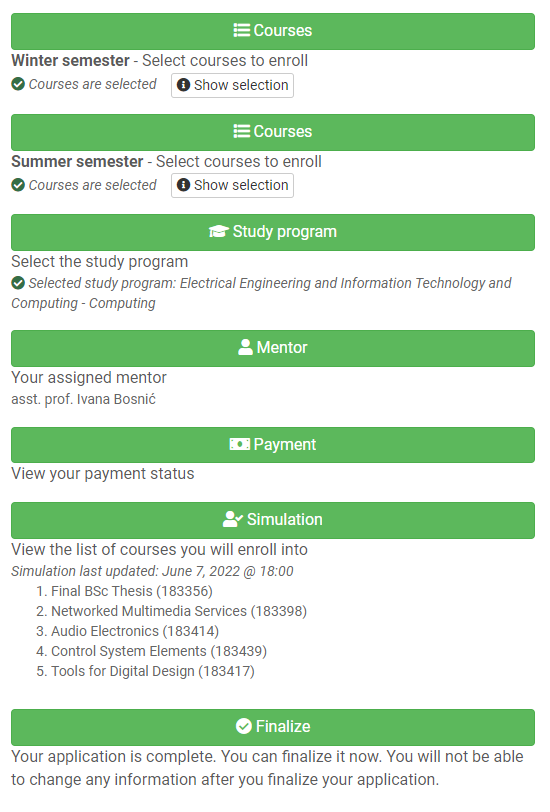
\includegraphics[scale=1]{stara/responzivnost.png}}
      \centering
      \caption{Prikaz responzivnosti i dvojezičnosti aplikacije}
    \end{figure}
    
    \section{Stari dizajn}
        \subsection{Opis starog dizajna}
        \textbf{Početna stranica}
        
        Početna stranica aplikacije sadrži gumbe za odabir predmeta po semestrima, gumb za odabir studijskog programa, gumb za odabir mentora (za studente koji upisuju treću godinu preddiplomskog studija ili prvu i drugu godinu diplomskog studija), gumb za pregled računa, gumb za simulaciju upisa semestra te gumb za predaju prijave čime je upis godine ili semestra zaključan. Neki od koraka upisa imaju naslov i/ili opis funkcionalnosti tog koraka. Na prvoj stranici upisa predmeta također se nalaze gumbi za brz prikaz odabranih predmeta za upis i zamjenskih predmeta.
        
        \begin{figure} [H]
          \fbox{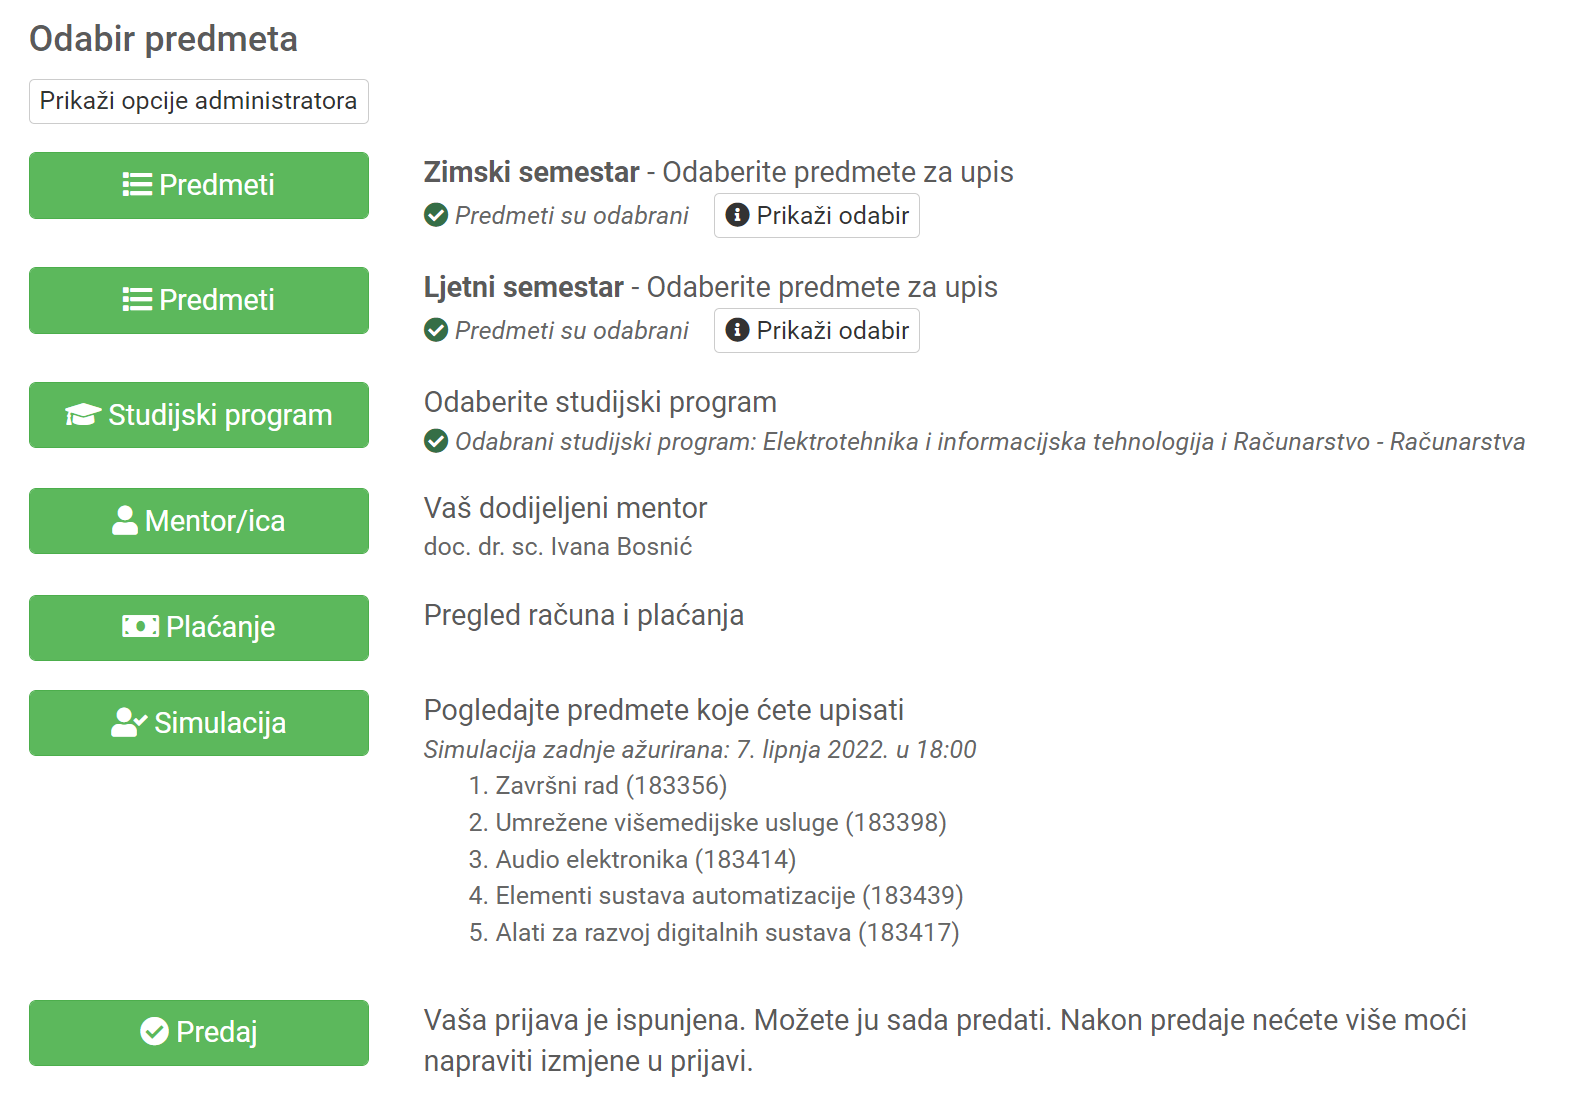
\includegraphics[scale=.5]{stara/index.png}}
          \centering
          \caption{Prikaz početne stranice trenutačne aplikacije}
        \end{figure}
        
        \noindent\textbf{Vaše informacije}
        
        S početne stranice pri upisu novog studija korisnik prvo bira opciju \textit{Vaše informacije} gdje popunjava formular s osobnim podacima i podacima svojih roditeljima te ostalim informacijama Fakultetu bitnim za upis.
        
        \noindent\textbf{Studijski program}
        
        Pri upisu na treću godinu preddiplomskog studija i prvu godinu diplomskog studija student mora odabrati studijski program koji upisuje. Stranica ima naslov \textit{Studijski program} s info-ikonicom. Ispod toga piše što korisnik na ovoj stranici treba napraviti i nakon toga nalaze se dva stupca. U prvom piše \textit{Studijski program}, a u drugom je prikazan popis studijskih programa od kojih student bira jedan. Na dnu stranice ponuđeni su gumbi \textit{Odustani} koji nas vodi na početnu stranicu i \textit{Spremi} koji sprema studentov odabir.
        
        \begin{figure} [H]
          \fbox{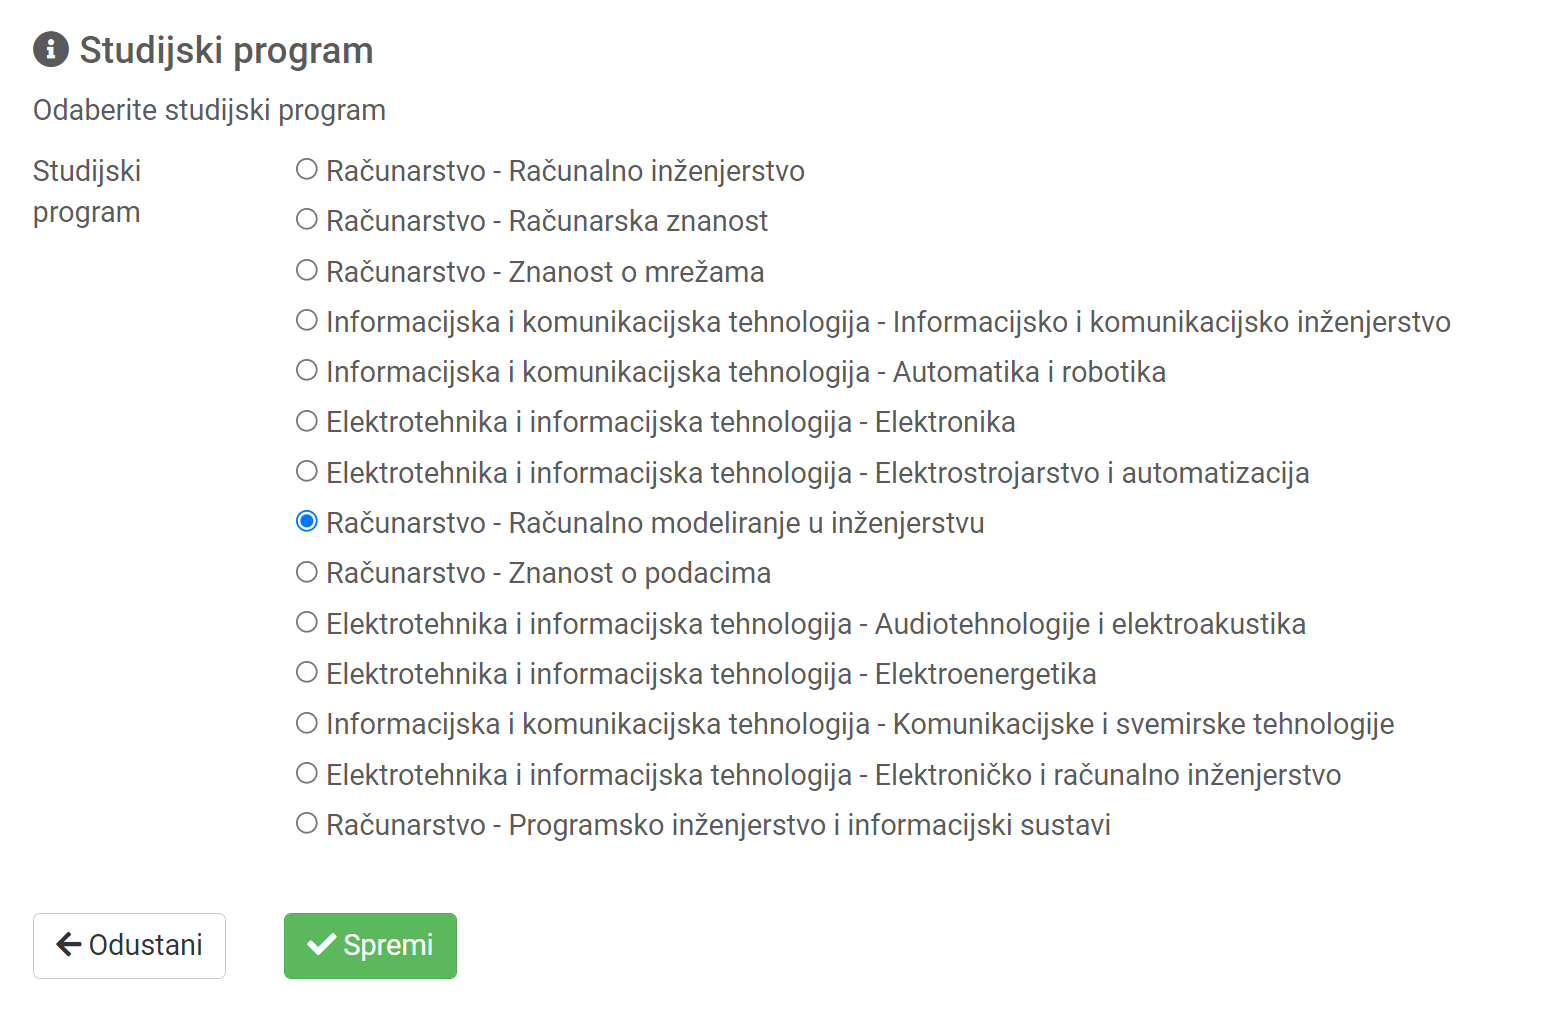
\includegraphics[scale=.5]{stara/program.png}}
          \centering
          \caption{Prikaz stranice odabira studijskog programa na diplomskom studiju}
        \end{figure}
        
        
        \noindent\textbf{Odabir predmeta}
        
        Klikom na gumb \textit{Predmeti} za određeni semestar (zimski ili ljetni), aplikacija korisnika vodi na stranicu gdje je nalazi popis dostupnih semestara u odabranoj godini (zimski ili ljetni). Ondje pod semestrom kojeg korisnik upisuje, ovisno o godini koju upisuje, može vidjeti odabrane predmete za upis i zamjenske predmete po semestrima.
        
        \begin{figure} [H]
          \fbox{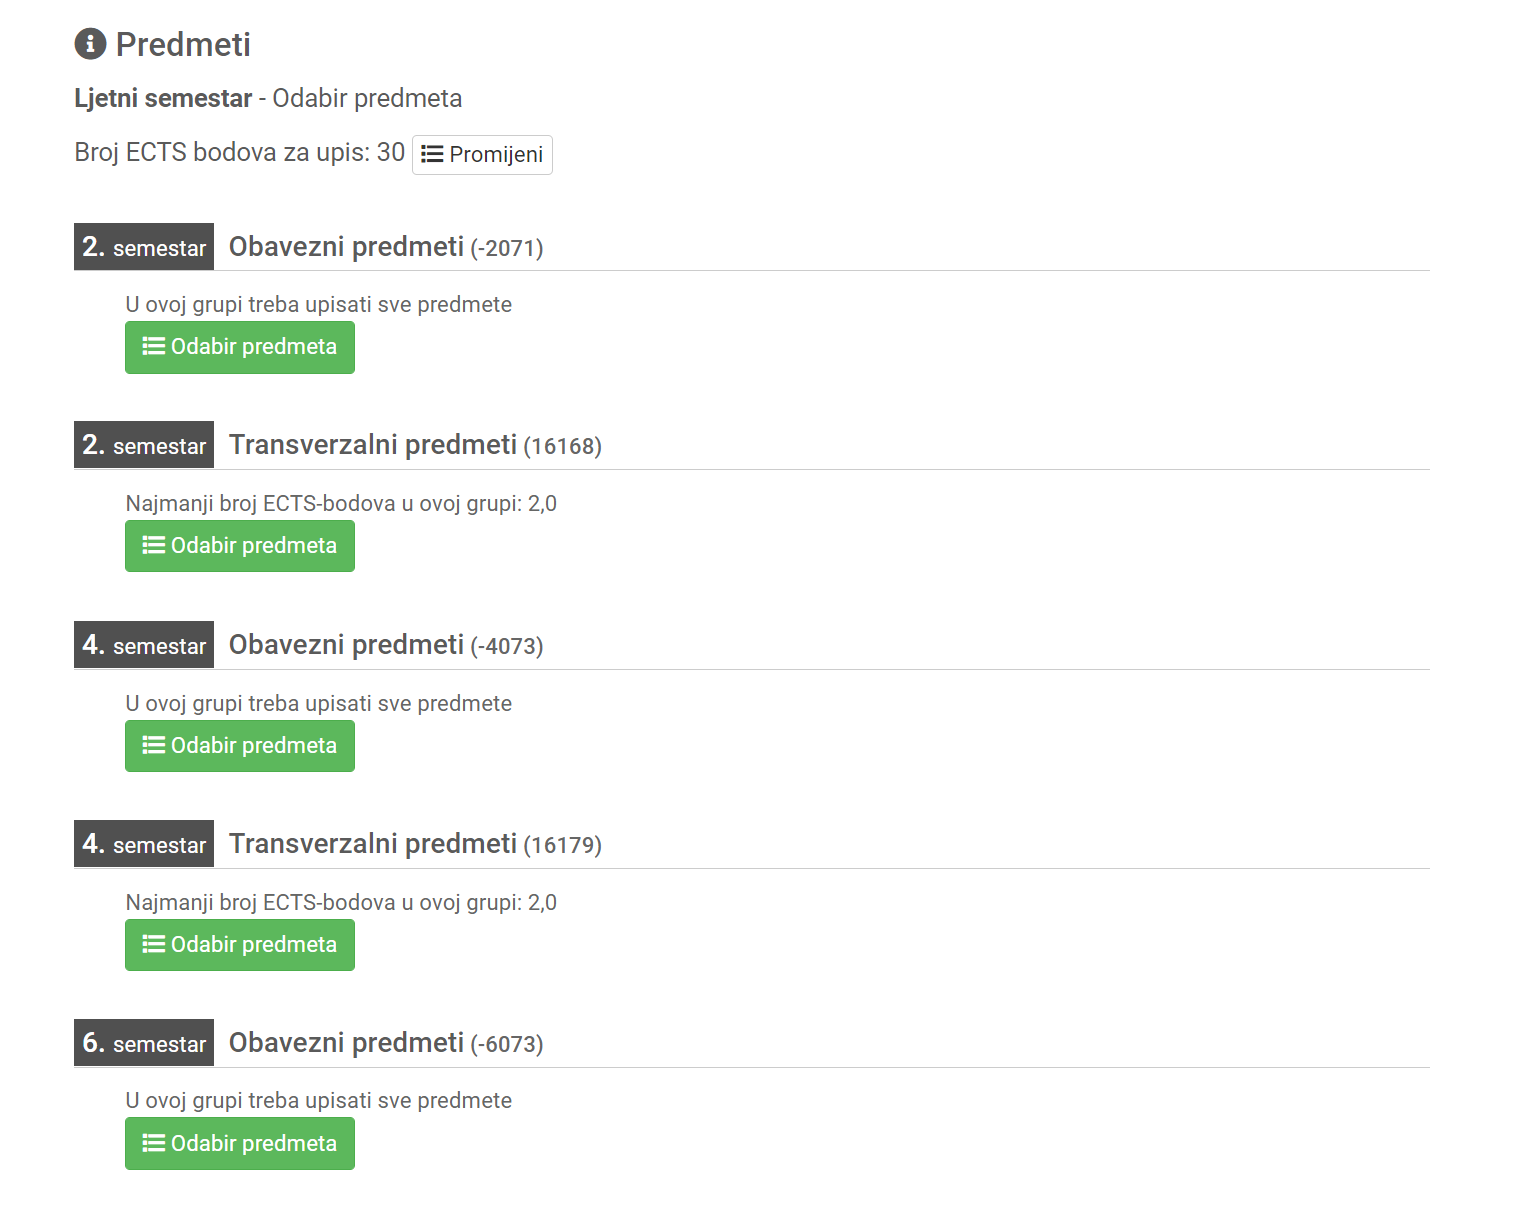
\includegraphics[scale=.5]{stara/courses_1.png}}
          \centering
          \caption{Prvi dio prikaza semestara u ljetnom semestru}
          \label{fig:courses_stara1}
        \end{figure}
        
        \begin{figure} [H]
          \fbox{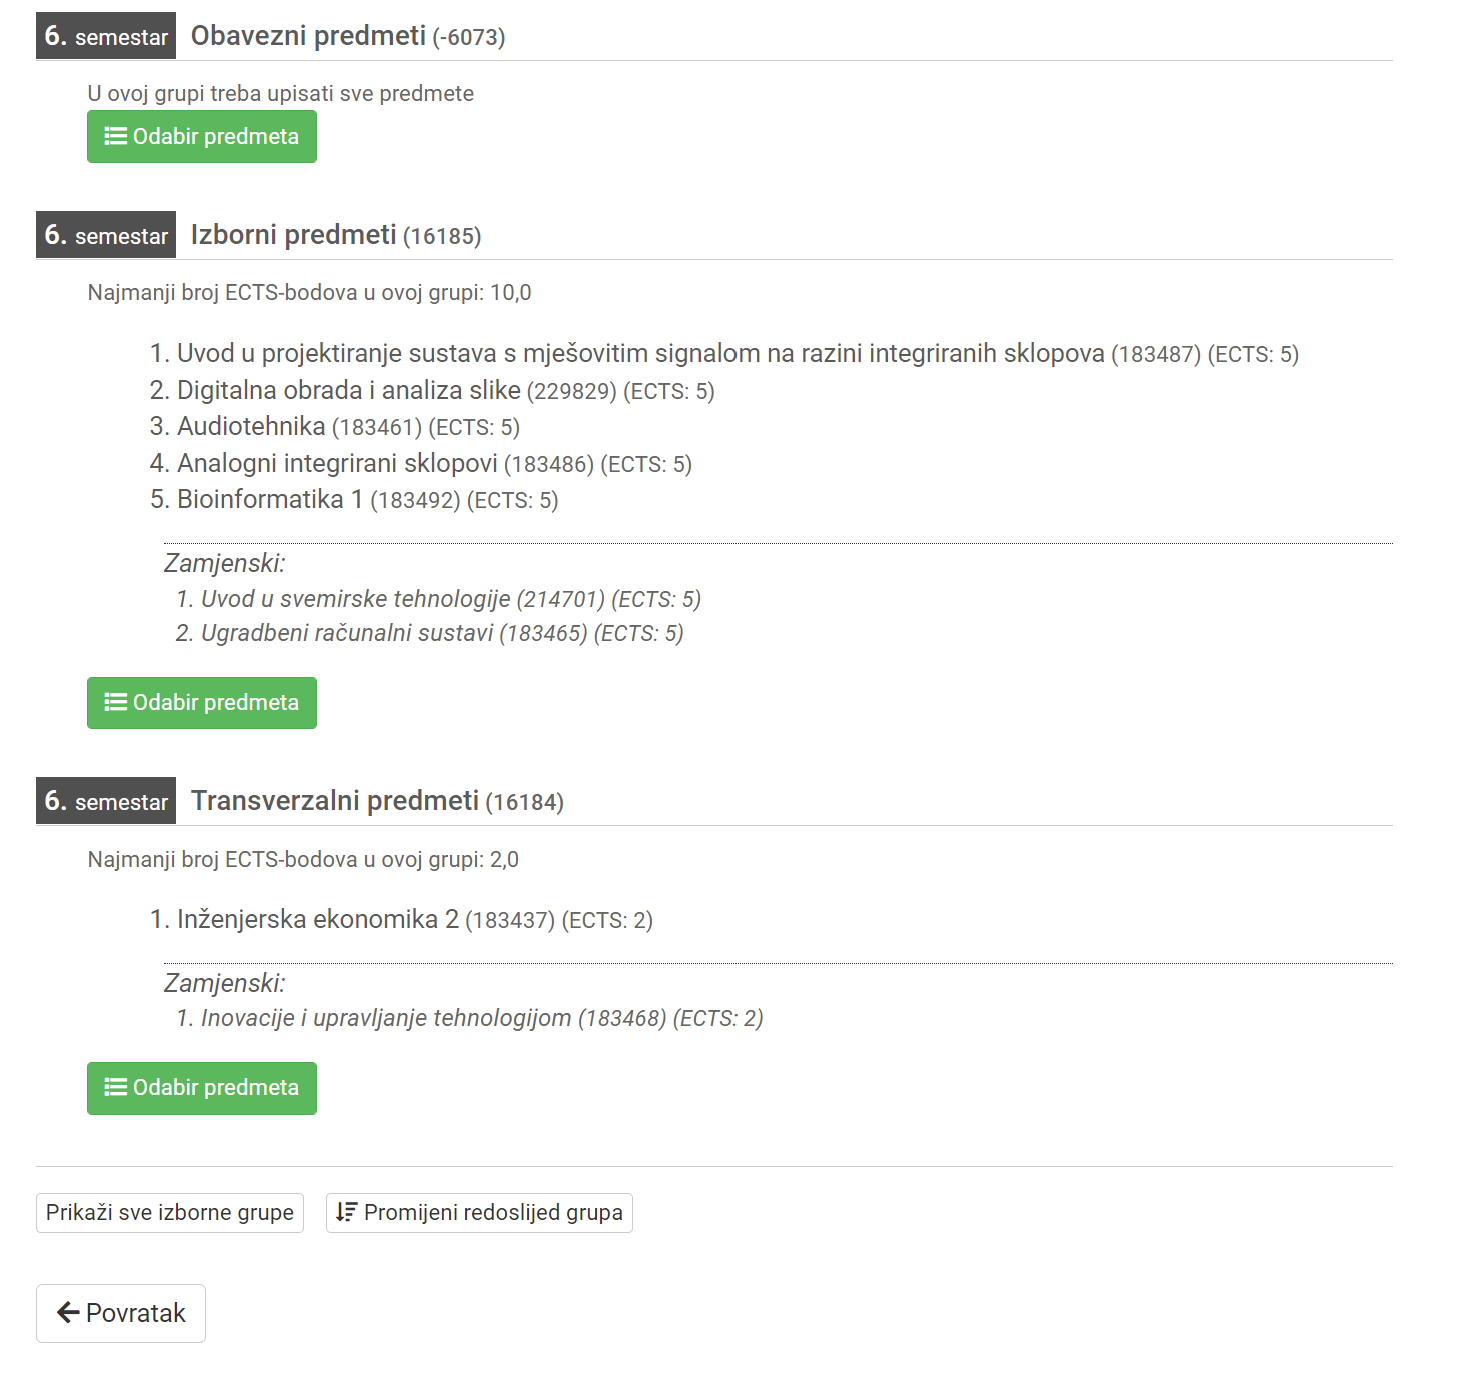
\includegraphics[scale=.5]{stara/courses_2.png}}
          \centering
          \caption{Drugi dio prikaza semestara u ljetnom semestru}
          \label{fig:courses_stara2}
        \end{figure}
        
        \noindent Iznad pregleda semestara naveden je broj ECTS-bodova koje korisnik upisuje u semestru i pored toga gumb za promjenu broja bodova (prikazano na slici \ref{fig:courses_stara1}) koji korisnika vodi na stranicu za biranje broja ECTS-bodova za upis u odabranom semestru.
        
        \begin{figure} [H]
          \fbox{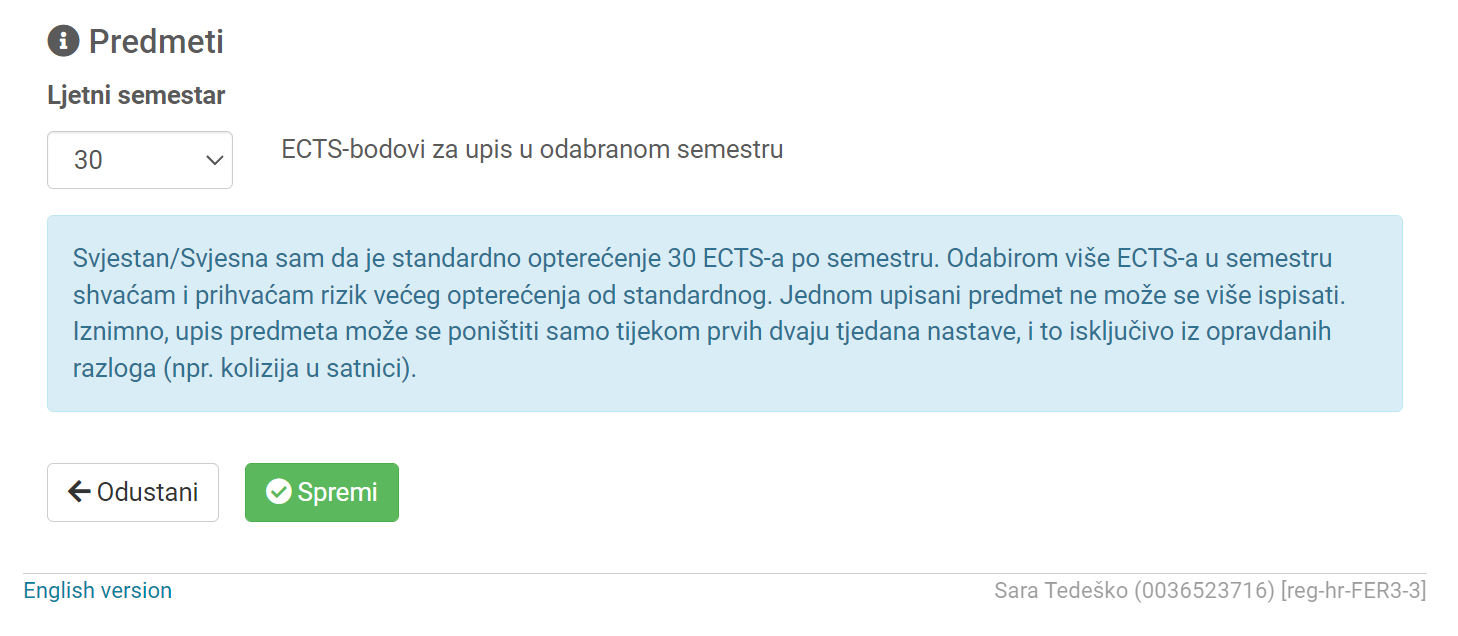
\includegraphics[scale=.5]{stara/ects.png}}
          \centering
          \caption{Prikaz odabranog broja ECTS-bodova za upis i stranice za njegovu promjenu}
        \end{figure}
        
        Ispod pregleda semestara nalaze se dodatni gumbi (prikazano na slici \ref{fig:courses_stara2}). Jedan služi za prikaz svih izbornih grupa, čime se uz obavezne, izborne i transverzalne predmete prikazuju i vještine te predmeti za iznimno uspješne studente. Drugi gumb nas vodi na novu stranicu gdje možemo klikom na strelice \textit{Gore} i \textit{Dolje} birati poredak prikaza grupa predmeta na prijašnjoj stranici. Ispod navedenih gumba imamo opciju povratka na prijašnju (početnu) stranicu.
        
        \begin{figure} [H]
          \fbox{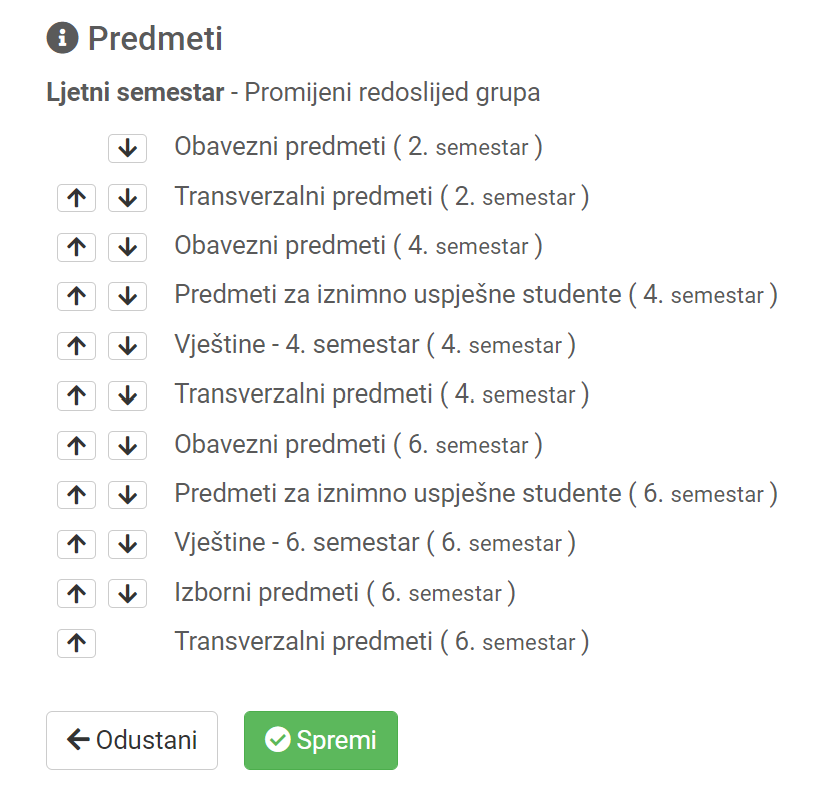
\includegraphics[scale=.6]{stara/group_order.png}}
          \centering
          \caption{Prikaz stranice za promjenu poretka grupa predmetu}
        \end{figure}
        
        Klikom na gumb \textit{Odabir predmeta} kod željenog semestra aplikacija korisnika vodi na novu stranicu gdje možemo birati predmete za upis i postaviti zamjenske predmete. Odabranim predmetima se strelicama \textit{Gore} i \textit{Dolje} može birati prioritet pri upisu. Za svaki odabrani predmet, osim mogućnosti mijenjanja prioriteta, imamo opciju uklanjanja predmeta s popisa za upis klikom na gumb \textit{Ukloni} s ikonicom kante za smeće. Na dnu stranice imamo opciju spremanja promjena odabira predmeta ili odustajanja, što korisnika vodi na prijašnju stranicu.
        
        \begin{figure} [H]
          \fbox{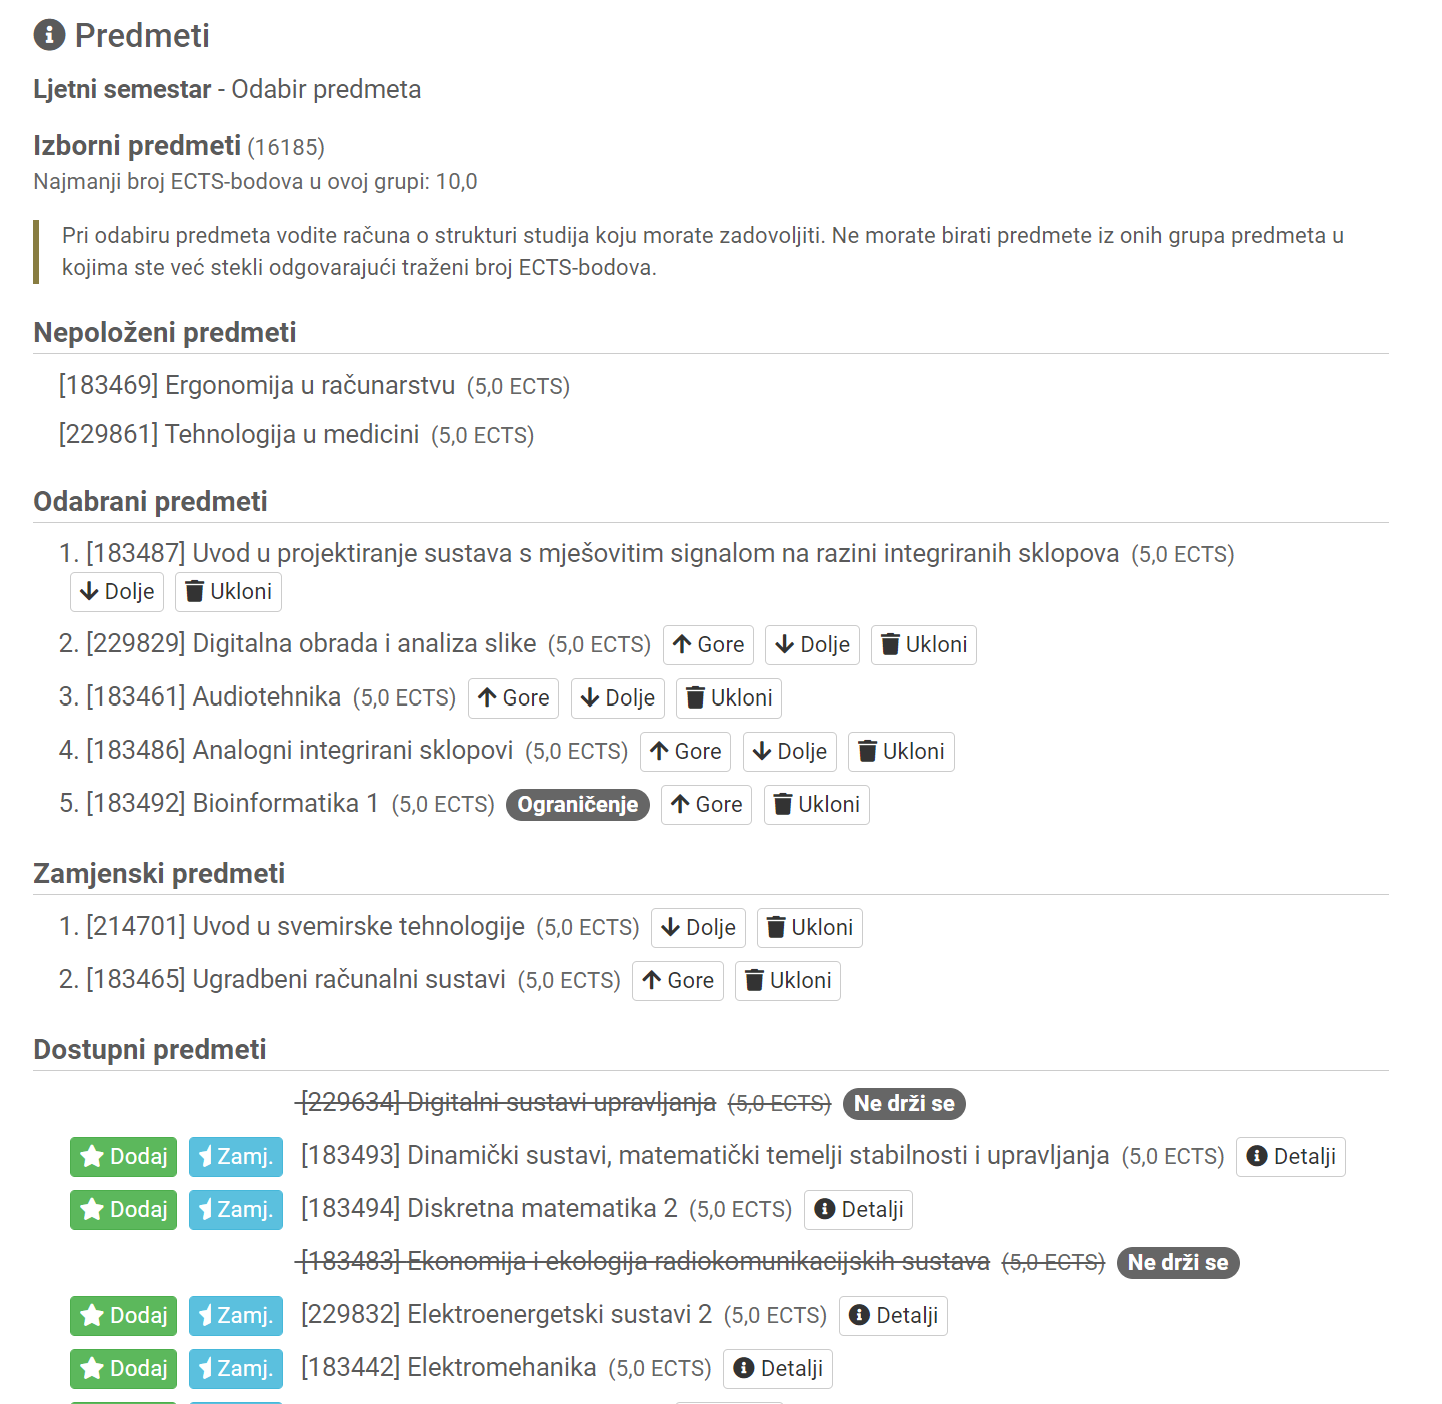
\includegraphics[scale=.5]{stara/selectcourses.png}}
          \centering
          \caption{Prikaz dijela stranice za biranje predmeta}
        \end{figure}
        
        \noindent\textbf{Mentor/ica}
        
        Klikom na gumb \textit{Mentor/ica} na početnoj stranici aplikacija korisnika vodi na odabir mentora. Ondje je prikazan popis odabranih mentora po prioritetu. Za svakog odabranog mentora postoje gumbi \textit{Gore} i \textit{Dolje} za mijenjanje prioriteta te gumb \textit{Ukloni} za micanje tog mentora s popisa odabranih. Ispod tog popisa nalazi se gumb za povratak na početnu stranicu i gumb za spremanje korisnikovog odabira. Također se na stranici nalazi polje za pretraživanje (\textit{search bar}) pomoću kojeg se mogu pretraživati mentori umjesto listanja po velikom popisu dostupnih mentora. Polje podržava upis imena, titule i kratice zavoda mentora. Za svakog mentora može se dobiti više informacija klikom na gumb \textit{Info} čime se otvara prozorčić personaliziran za tog mentora.
        
        
        \begin{figure} [H]
          \fbox{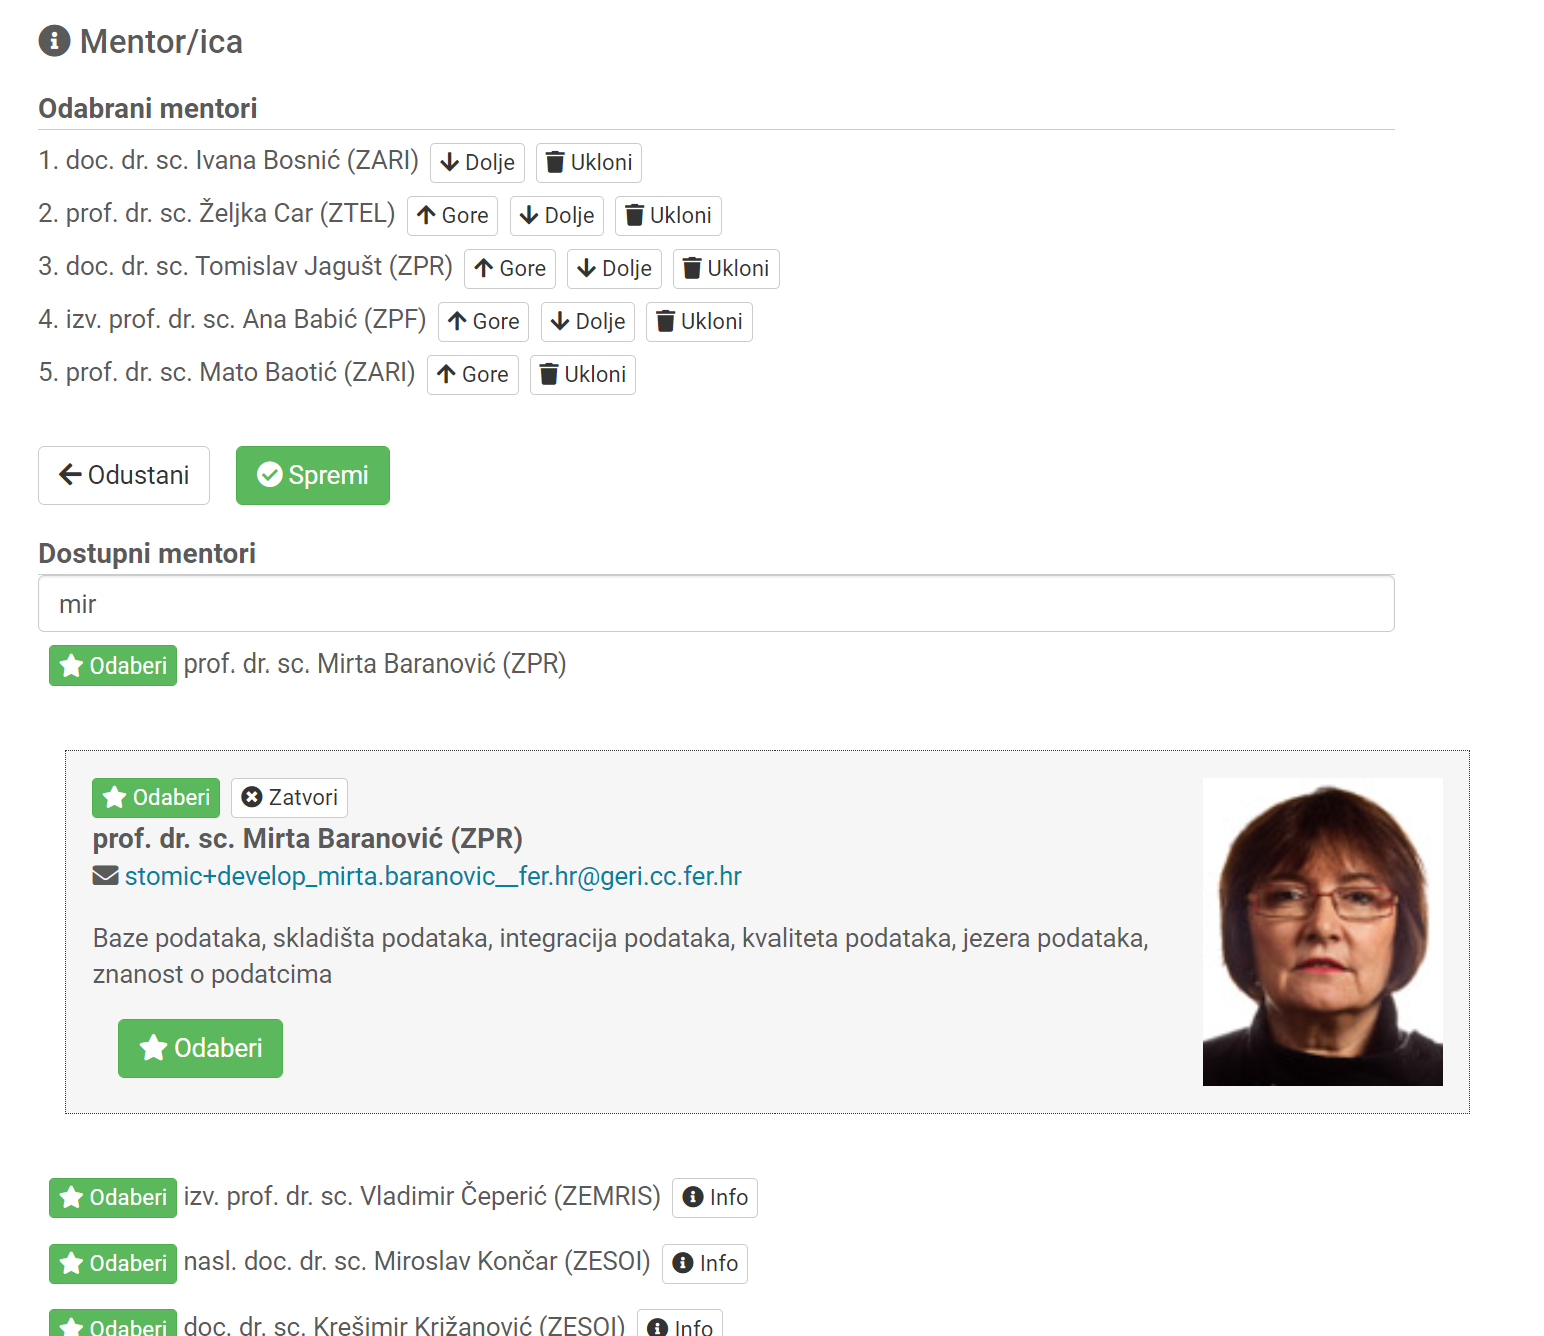
\includegraphics[scale=.5]{stara/mentor.png}}
          \centering
          \caption{Prikaz dijela stranice za biranje mentora}
        \end{figure}
        
        \noindent\textbf{Plaćanje}
        
        Na stranici plaćanja, do koje student dolazi s početne stranice, studenti mogu pregledati svoje račune. Vidi se ukupan iznos dûga studenta i tablica s računima gdje se računi mogu preuzeti na uređaj koji student trenutno koristi. Povratak na početnu stranicu obavlja se klikom na gumb \textit{Odustani}.
        
        \begin{figure} [H]
          \fbox{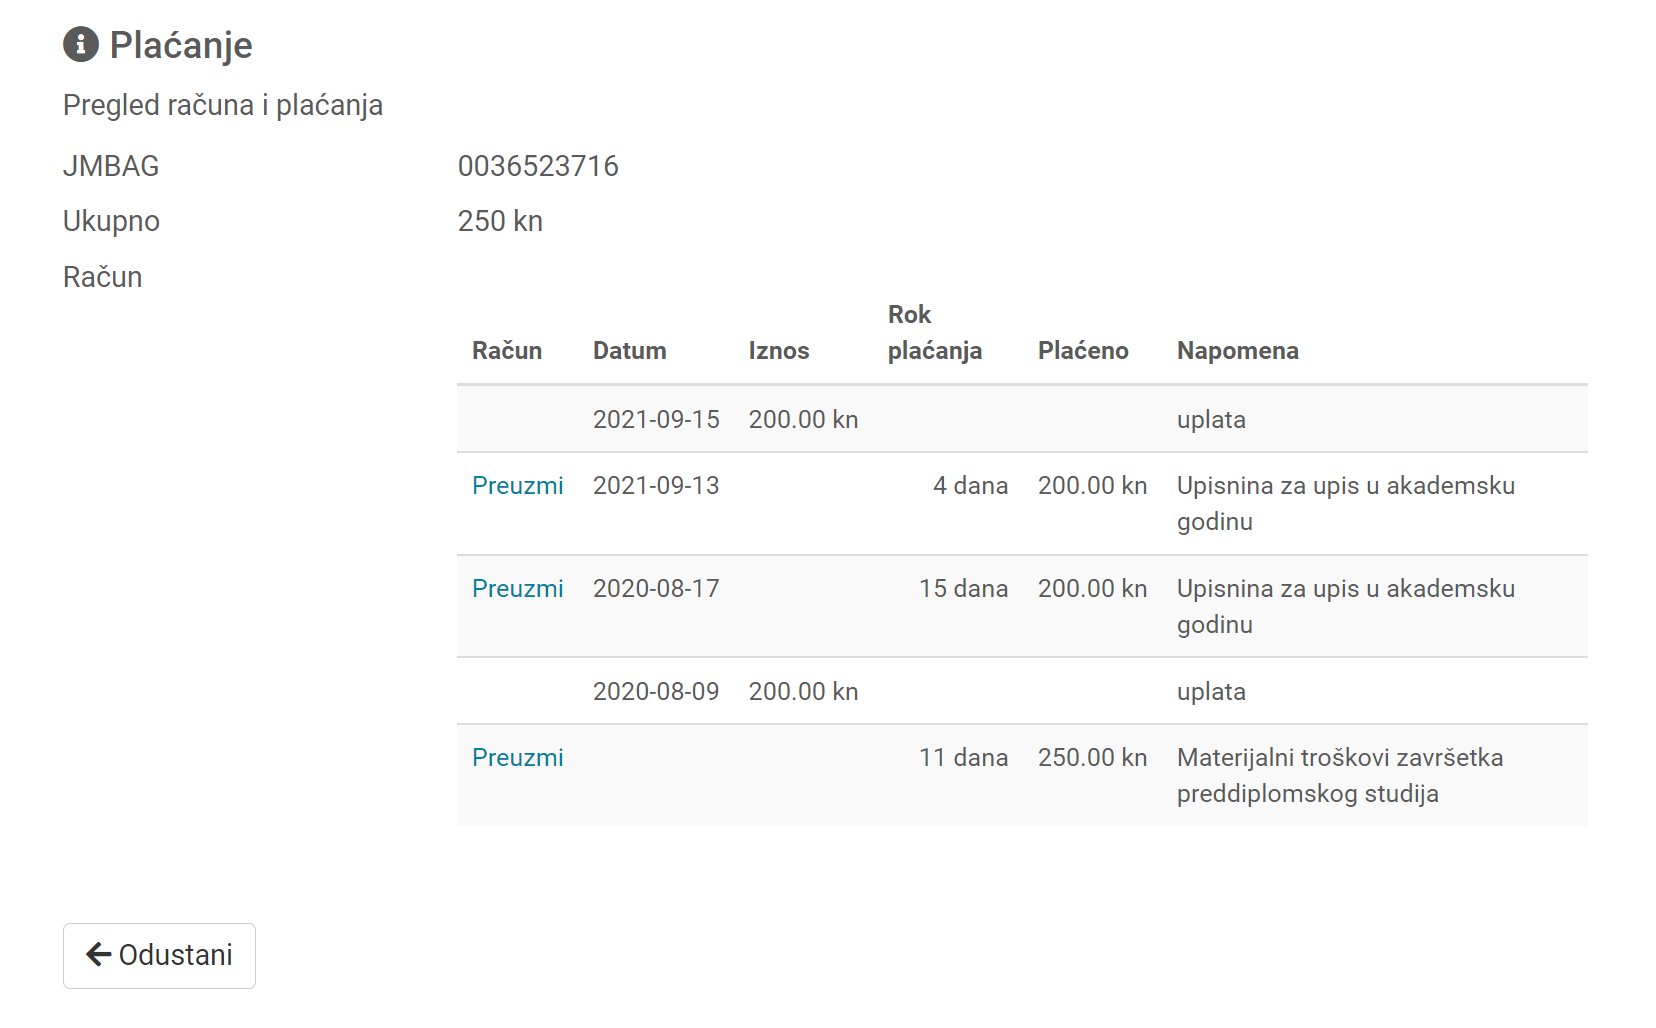
\includegraphics[scale=.4]{stara/payment.png}}
          \centering
          \caption{Prikaz stranice plaćanja}
        \end{figure}
        
        
        
        \vspace{\baselineskip}
        \bigbreak
        \noindent\textbf{Simulacija}
        
        Na početnoj stranici gumb \textit{Simulacija} korisnika vodi na stranicu gdje može vidjeti koji predmeti po grupama predmeta će mu biti upisani s obzirom na njegov odabir i postavljen broj ECTS-bodova. Na početku stranice nalazi se gumb za ažuriranje simulacije, a na samom dnu gumb za povratak na prijašnju, odnosno početnu stranicu.
        
        \begin{figure} [H]
          \fbox{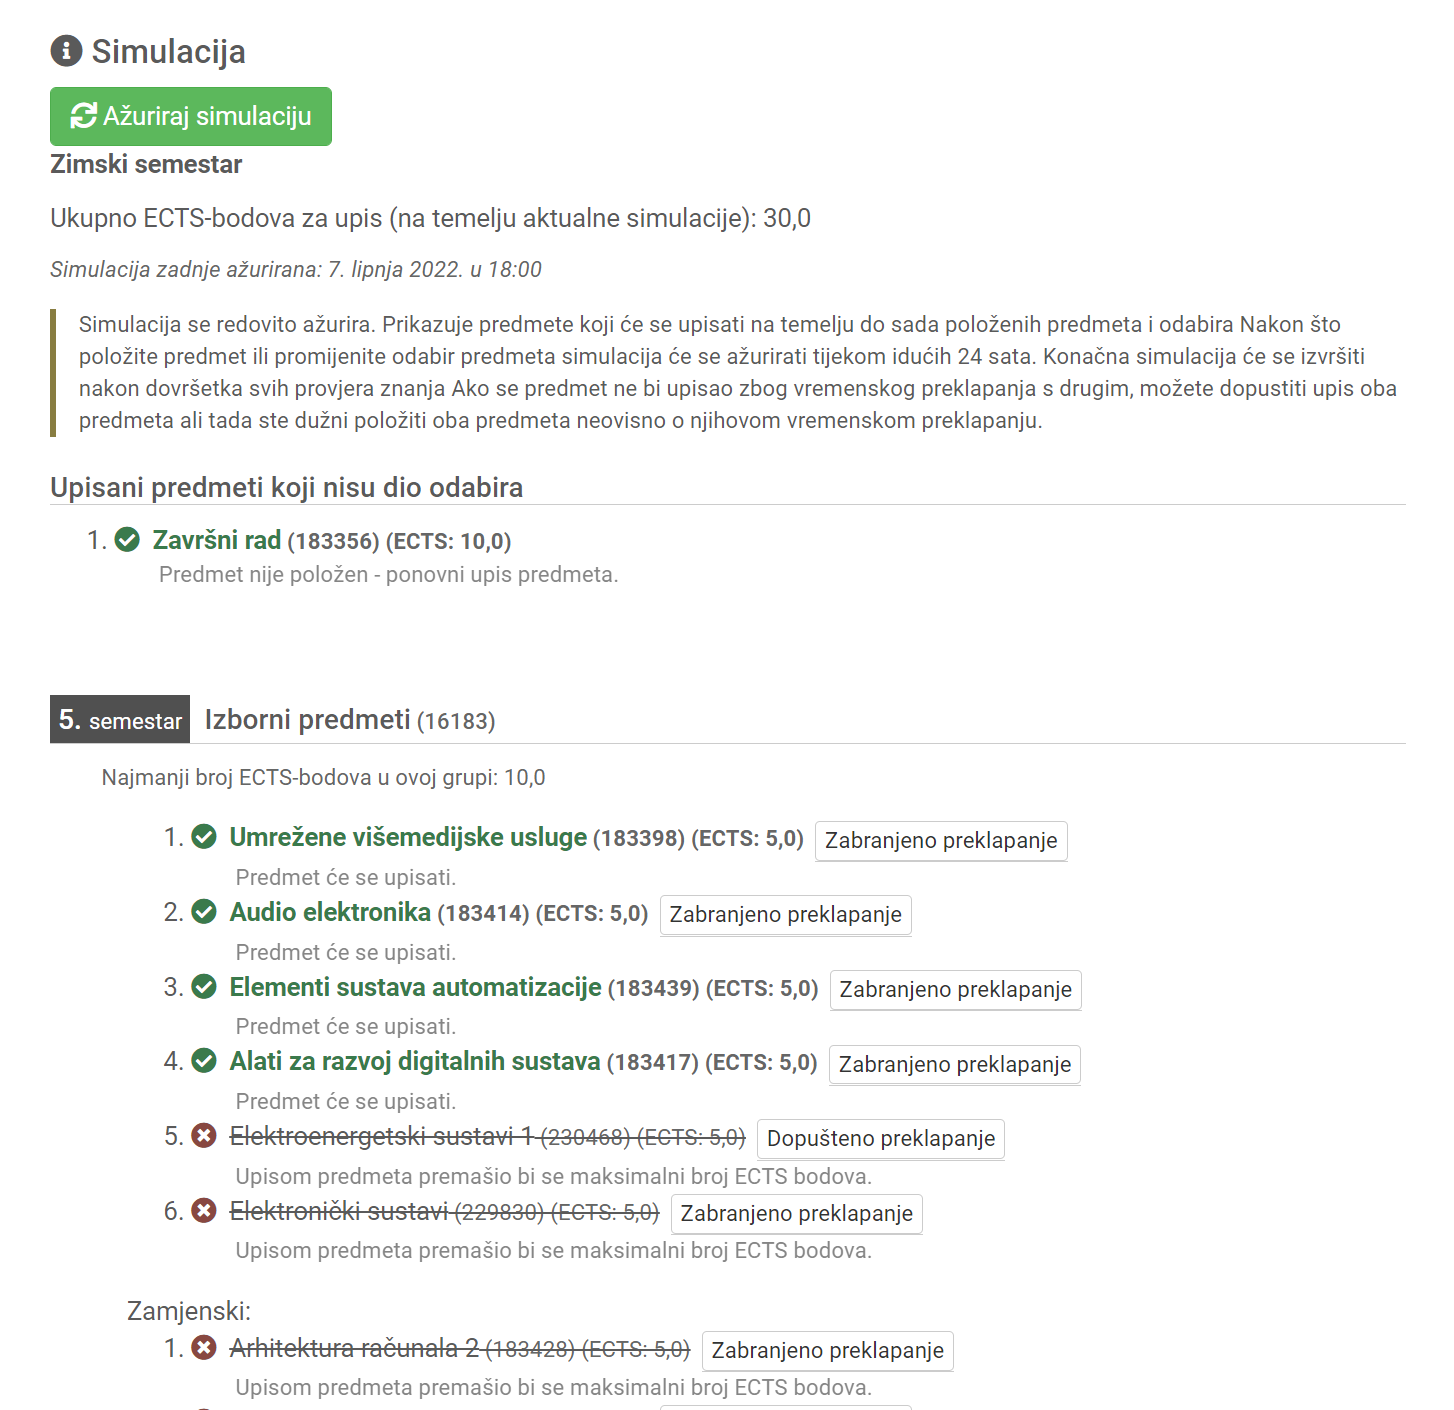
\includegraphics[scale=.5]{stara/simulation.png}}
          \centering
          \caption{Prikaz dijela stranice simulacije}
        \end{figure}


        \subsection{Evaluacija starog dizajna}
        Procjenu dizajna obavljalo je petero studenata. Zbog različitosti preferencija ljudi broj pet je idealan broj osoba za procjenu. Broj osoba je dovoljno velik da se mogu otkriti skoro svi problemi aplikacija.
        
        Neke od primjedbi bile su univerzalne u skupini studenata za procjenu, dok je druge spomenule samo jedne ili dvije osobe.
        
        Jedna od čestih primjedbi među studentima bila je kaotičnost izgleda \textbf{popisa odabranih i zamjenskih predmeta}. Pozicioniranje gumba promjene poretka i uklanjanja predmeta ovisilo je o duljini naziva predmeta i zbog toga nisu konzistentno jedan ispod drugog. Kako promjena nije popraćena animacijom, zamjena redoslijeda predmeta bila je trenutačna. Ovo dizajn čini neatraktivnim i težim za korištenje jer bi korisnik trebao tražiti gdje se koji gumb nalazi sada nakon promjene poretka.
        Uz to, na prvom mjestu, kao najvažniji podatak, napisan je ID predmeta umjesto da student prvo vidi naziv predmeta po kojem predmete međusobno razlikuje.
        
        Nekoliko studenata imalo je i primjedbu za oznake \textit{Ograničenje}, \textit{Ne drži se} i \textit{Nije moguće upisati}. Oznaka je previše upečatljiva i sliči na gumb. Korisnikova intuicija mu govori kako bi se nešto trebalo dogoditi ako dođe mišem na oznaku i klikne je. Međutim, ovo je samo oznaka i pozicioniranjem miša na nju neće se ništa dogoditi.
        
        Druga jednoglasna primjedba bila je povezana sa \textbf{stranicom prikaza semestara}. Na stranici su prikazani sve grupe predmeta za svaki semestar u odabranom dobu (zimski ili ljetni) na upisanom studiju. Ispod svake od grupa piše koliko ECTS-bodova je potrebno upisati. Ovo izaziva zbunjenost jer djeluje kao da je potrebno birati predmete iz drugog semestra kada upisujemo šesti. Ova stranica bila je velik razlog davanja niže ocjene korisničkom iskustvu aplikacije. Također na toj stranici dio studenata nije primijetio opciju \textbf{promjene broja ECTS-bodova} za upis. Ovo može biti veliki problem ako student želi upisati više od 30 ECTS-bodova u semestru i simulacija mu pokazuje da to ne može učiniti jer je maksimalan broj odabran jednak 30.
        
        Studenti su ocijenili svoje iskustvo s odabirom predmeta te je prosječna ocjena \textbf{3.8/5}.
        
        \begin{figure} [H]
          \fbox{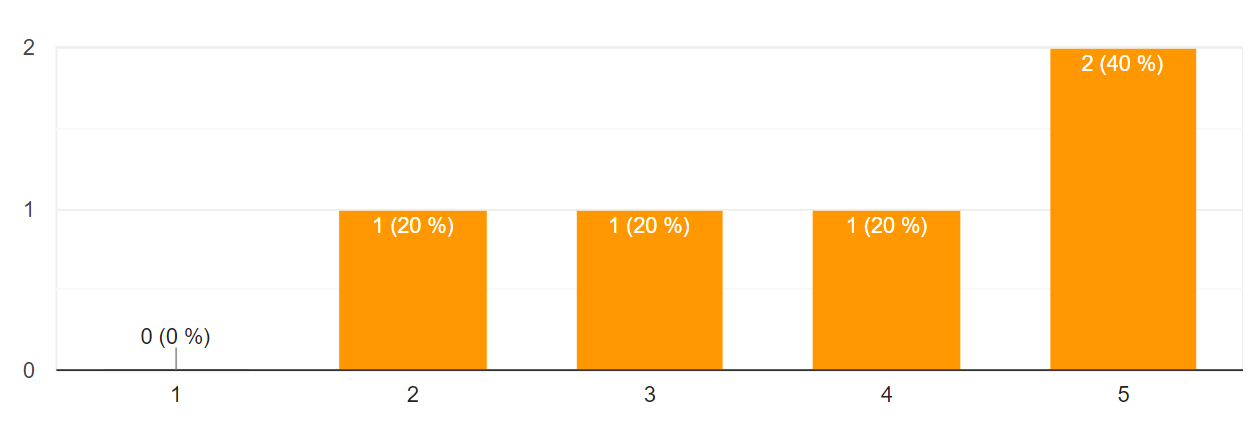
\includegraphics[scale=.6]{stara/courses_ocjena.png}}
          \centering
          \caption{Ocjene korisničkog iskustva prikaza semestara i biranja predmeta na aplikaciji starog dizajna}
        \end{figure}
        
        Treći komentar zaprimljen od svakog od pet studenata odnosio se na \textbf{stranicu plaćanja}. Naime tablica računa se sastoji od dva puta više redaka nego što ima računa. Ovo je zato što se dva retka tablice odnose na jedno plaćanje. Jedan redak predstavlja račun, a drugi studentovu uplatu. Ova stranica dobila je najgore ocjene od studenata i njihov prosjek je \textbf{1.8/5}.
        
        \begin{figure} [H]
          \fbox{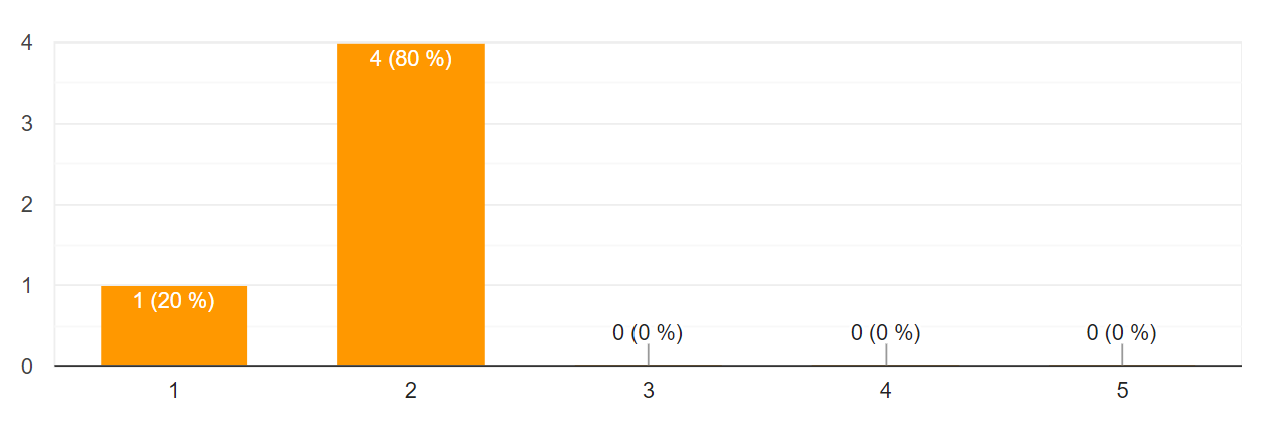
\includegraphics[scale=.6]{stara/placanje_ocjena.png}}
          \centering
          \caption{Ocjene korisničkog iskustva sa stranicom plaćanja na aplikaciji starog dizajna}
        \end{figure}
        
        Posljednja izražena primjedba vezana je uz \textbf{simulaciju}. Na stranici postoji previše komentara koji odvlače pozornost od najbitnije stvari simulacije, a to je provjeriti koji predmeti će studentu biti upisani. Također postoji nejasnoća značenja termina \textit{preklapanje} u kontekstu preklapanja predmeta.
        
        Studenti su na kraju evaluacije trebali ocijeniti svoje iskustvo korištenja aplikacije. Prosječna dana ocjena za postojeću aplikaciju je \textbf{3.2/5}.
        
        \begin{figure} [H]
          \fbox{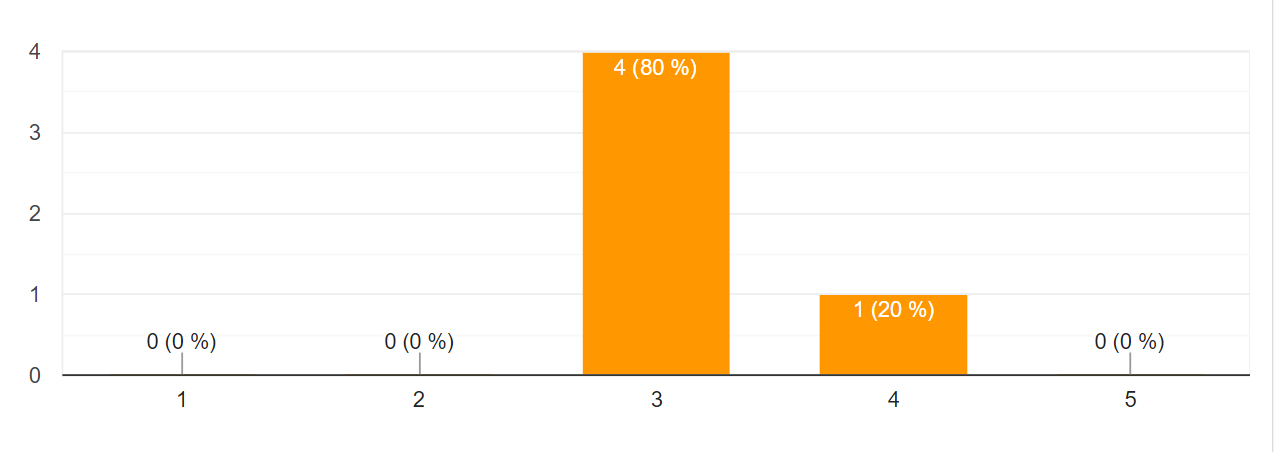
\includegraphics[scale=.6]{stara/overall.png}}
          \centering
          \caption{Ocjene korisničkog iskustva aplikacije starog dizajna}
        \end{figure}
        
        
    \section{Poboljšani dizajn}
    
        \subsection{Opis poboljšanog dizajna}
        Na svim stranicama promijenjeni su naslovi kako bi bili u skladu s onime što prikazuju te su dodane ikonice koje odgovaraju onima na gumbima na početnoj stranici. Gdje god se u aplikaciji spominje određeni predmet, prikaz je promijenjen da naziv predmeta dolazi prvi, a nakon njega ID predmeta. Studenti predmete pamte po njihovim naslovima, a ne ID-u. Zbog toga im je bitnije prvo vidjeti naslov. Svim gumbima koji nisu obojani (gumbima s bijelom pozadinom) dodan je \textbf{okvir tamnije boje} zbog bolje vidljivosti.
        
        U cijeloj aplikaciji korištena zelena nijansa gumba zamijenjena je u plavu boju kako bi se bolje uklopila u ostatak FER-ove stranice gdje je ova nijansa plave korištena kao boja gumba. Na mjestima na kojima je zelena boja ostavljena, promijenjena joj je nijansa kako bi bila u skladu s razinom AA kriterija WCAG 2.0 o kontrastu boja teksta, elemenata i pozadina. Osim boje, korišteni su i drugi načini razlikovanja elemenata na stranicama kako bi i osobama koje ne vide boje bilo jasno da postoji razlika između elemenata. Iz tog razloga, na početnoj stranici dodana je linija koja odvaja gumb za predaju od ostatka postupka prijave. Na gumb prijave također je dodana animacija \textit{fadeInLeft} (iz biblioteke animate.css) koja se prikazuje pri učitavanju stranice za dodatno razlikovanje i stavljanje važnosti na posljednji gumb. Gumb \textit{Predaj} zelene je boje kako bi se primijenilo djelovanje \textbf{Von Restorffovog efekta} Gestalt pravca psihologije. U skupini sličnih elemenata onaj element koji je drugačiji od ostalih najčešće ostaje zapamćen.
        
        Pri promjeni stranica koristi se animacija horizontalne translacije ulijevo pri izlazu sa stranice te onda udesno pri ulazu na novu stranicu. Za ovo je korištena komponenta \textit{Transition}. Opširnije objašnjenje nalazi se u poglavlju 5, \textit{Izrada poboljšanog i novog modula}.
        
        Na početnoj stranici \textbf{podebljani su naslovi} za svaki od koraka upisa kako bi korisniku bilo jasnije da se radi o novom dijelu upisa. Na dijelovima gdje se do sada nisu nalazili dodani su naslovi i \textbf{kratki opisi} na dijelovima gdje se on nije nalazio za bolje razumijevanje čemu ovaj dio prijave služi i zbog konzistentnosti dizajna. Uz to, postavljen je jednak razmak između svakog dijela prijave što prije nije bio slučaj.
        
        Gumb za odabir studijskog programa stavljen je prije gumba za biranje predmeta po semestrima jer je za biranje predmeta prvo potrebno odabrati studijski program kojeg upisujemo (ako on već nije odabran ranije).
        
        Gumbi \textit{Predmeti} preimenovani su u \textit{Upiši predmete} po primjedbama iz istraživanja. Tekst na gumbu \textit{Prikaži odabir} promijenjen je u \textit{Prikaži moj odabir} zbog bolje jasnoće njegove svrhe. Na njega su dodane animacije \textit{fadeInDown} kada korisnik odabere pregledati svoj odabir i \textit{fadeOutUp} za zatvaranje pregleda odabira.
        
        \begin{figure} [H]
          \fbox{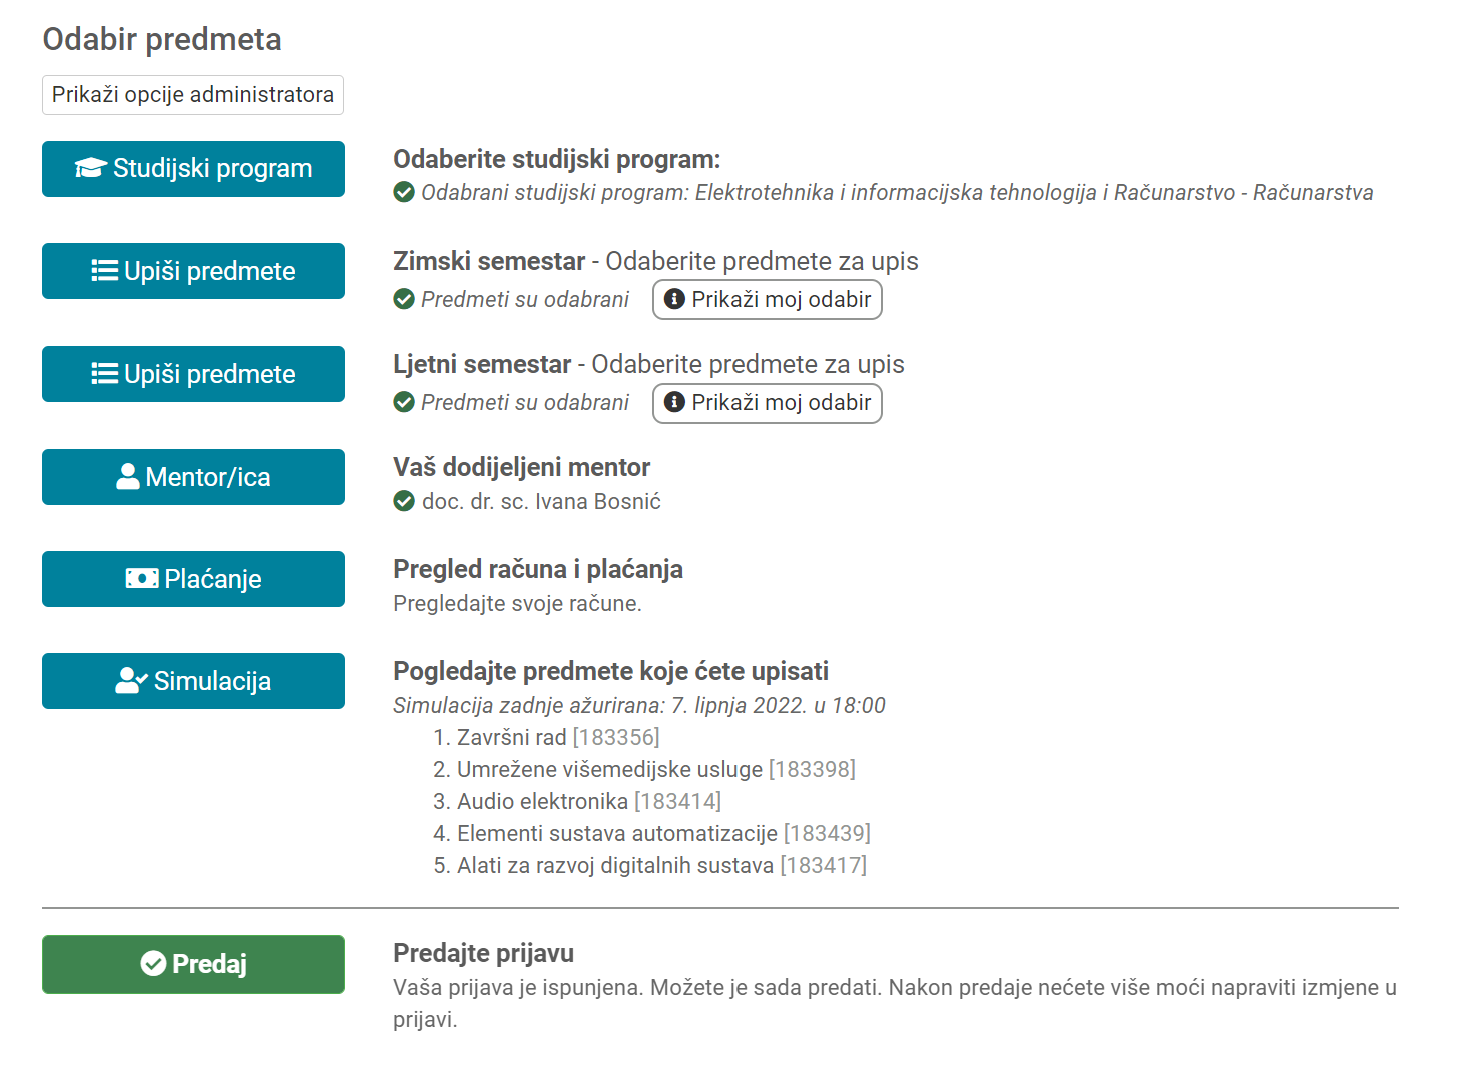
\includegraphics[scale=.5]{poboljsana/index.png}}
          \centering
          \caption{Promijenjena početna stranica aplikacije}
        \end{figure}
        
        Modul je uporabom responzivnog dizajna prilagođen za uređaje manjih dimenzija. Također podržava mogućnost prikaza dvojezičnog sadržaja.
        
        \begin{figure} [H]
          \fbox{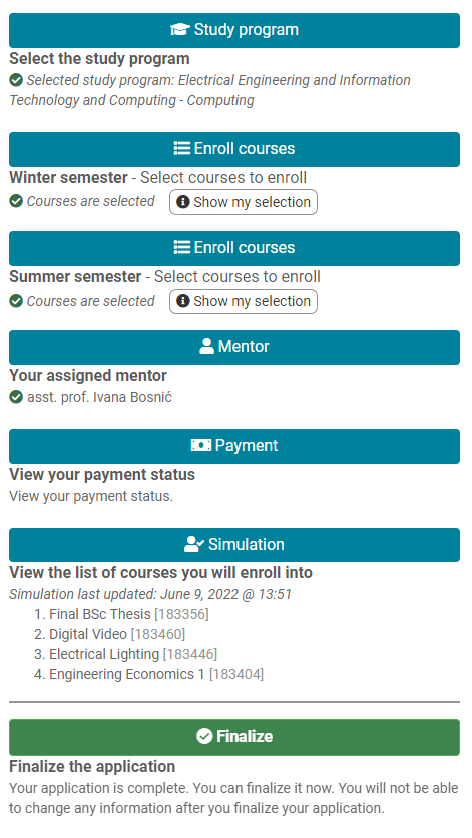
\includegraphics[scale=.7]{poboljsana/responzivnost.png}}
          \centering
          \caption{Prikaz responzivnosti}
        \end{figure}
        
        \vspace{\baselineskip}
        \bigbreak
        \noindent\textbf{Vaše informacije}
        
        Pri upisu na prvu godinu studija prvi gumb za odabir na početnoj stranici je \textit{Vaše informacije} gdje korisnik popunjava obrazac s osobnim podacima i podacima svojih roditeljima i ostalim informacijama Fakultetu bitnim za upis. Naslov stranice je podebljan i info-ikonica zamijenjena je ikonicom kućice. Opisi vezani za unos određenog podatka prebačeni su iznad polja za unos umjesto ispod kako su do sada bili. Ovo je napravljeno zbog bolje pristupačnosti stranice osobama koje koriste \textbf{čitače ekrana}. Naime čitač će na ovaj način korisniku prvo pročitati opis i objašnjenje polja prije nego dođe do dijela za unos. Slika ove stranice nije prikazana iz sigurnosnih razloga.
        \linebreak\linebreak
        \noindent\textbf{Studijski program}
        
        Na stranici biranja studijskog programa uklonjena je oznaka \textit{Studijski program} jer naslov i tekst ispod njega jasno objašnjavaju što korisnik ovdje odabire. Kako je oznaka uklonjena, ponuđeni izbori programa uvučeni su ulijevo.
        
        \begin{figure} [H]
          \fbox{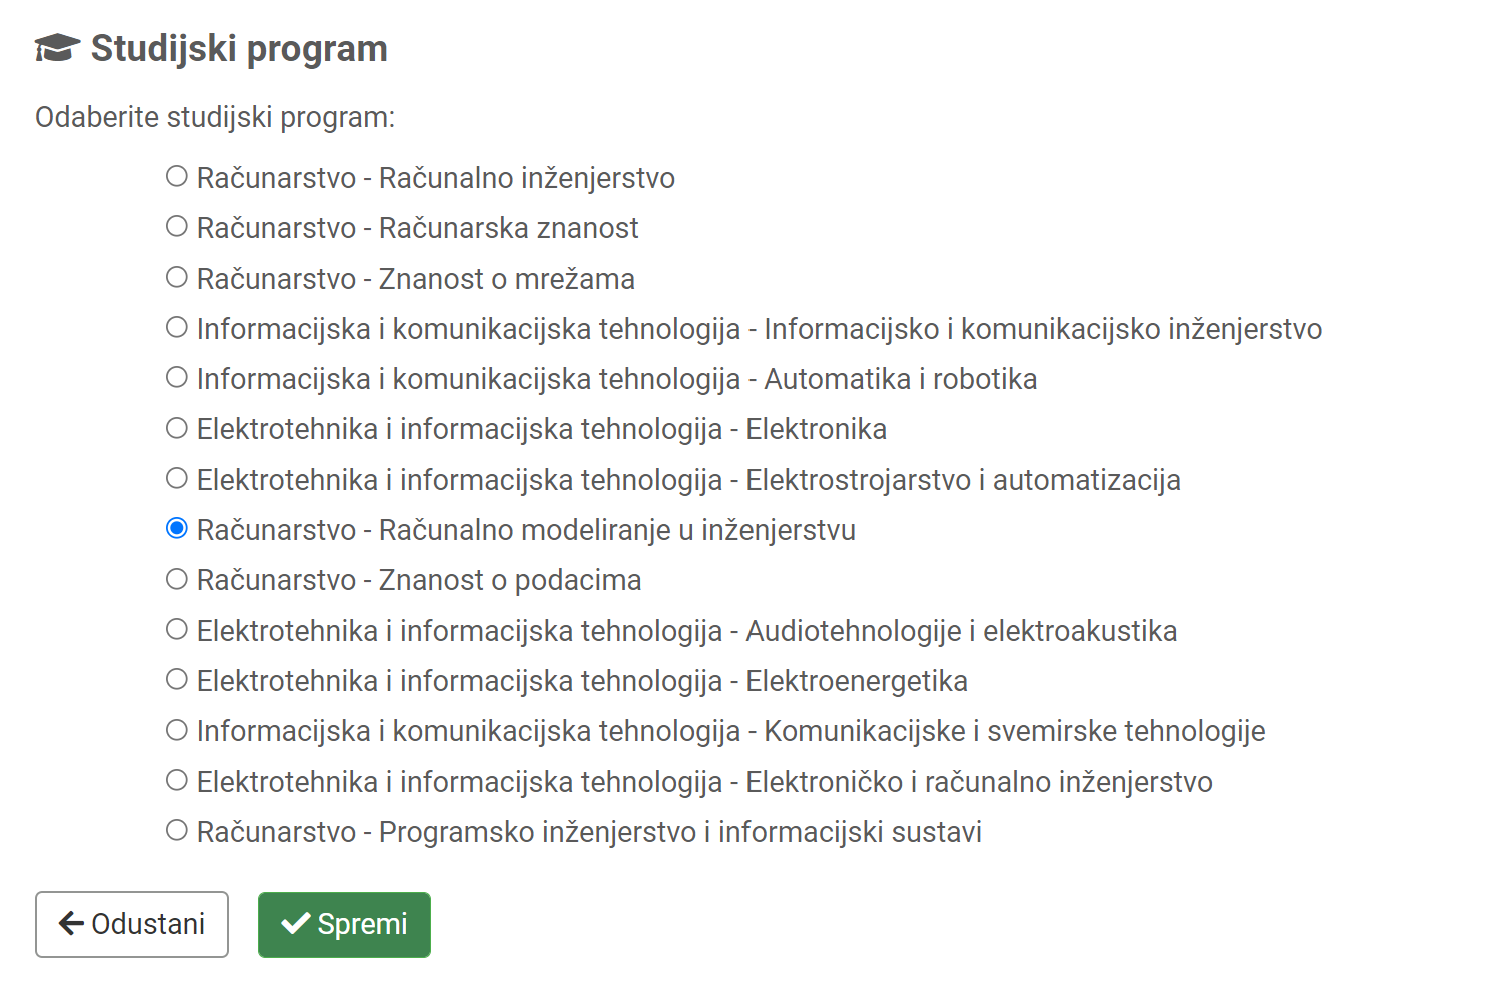
\includegraphics[scale=.5]{poboljsana/program.png}}
          \centering
          \caption{Promijenjena stranica odabira studijskog programa na diplomskom studiju}
        \end{figure}

        
        \noindent\textbf{Odabir predmeta}
        
        Pri upisu godine na početnoj stranici ponuđene su opcije za upis predmeta u ljetnom i zimskom semestru. Odabirom semestra dolazimo na stranicu s popisom grupa predmeta po semestru. Glavni uočeni problemi na ovoj stranici bili su prikaz semestara i grupa predmeta iz kojih su studenti već položili sve predmete te opcija promjene broja ECTS-bodova za upis u semestru koju velik dio studenata nije primijetio. Na početak je dodana poruka koja objašnjava zašto su prikazani već završeni semestri. Ispred broja odabranih ECTS-bodova za upis dodana je ikona uskličnika u trokutu kako bi se privukla pozornost studenata na ovaj dio stranice. Također je podebljan odabrani broj bodova.
        
        \begin{figure} [H]
          \fbox{
\includegraphics[scale=.5]{poboljsana/ects.png}}
          \centering
          \caption{Promijenjena stranica promjene ECTS-bodova za ljetni semestar}
        \end{figure}
        
        Uz to, studenti su tijekom procjene starog dizajna komentirali nepreglednost stranice. U ovu svrhu sav tekst ispod grupe predmeta po semestru uvučen je jednako duboko kako se ne bi stvarala dodatna nepotrebna hijerarhija koja je prije bila prisutna. Nazivi odabranih predmeta u grupi su podebljani, a sa zamjenskih predmeta je uklonjen stil kurziv iz razloga što tako stiliziran tekst otežava čitanje ljudima s disleksijom. S dna stranice uklonjena je mogućnost promjene redoslijeda prikaza grupa predmeta na stranici jer njeno uklanjanje ni na koji način ne pogoršava korisničko iskustvo. Za bolje vidljivo odvajanje grupa predmeta povećan je njihov međusobni razmak te je između različitih semestara dodana je blago siva pozadina na prikaz svakog drugog semestra.
        
        \begin{figure} [H]
          \fbox{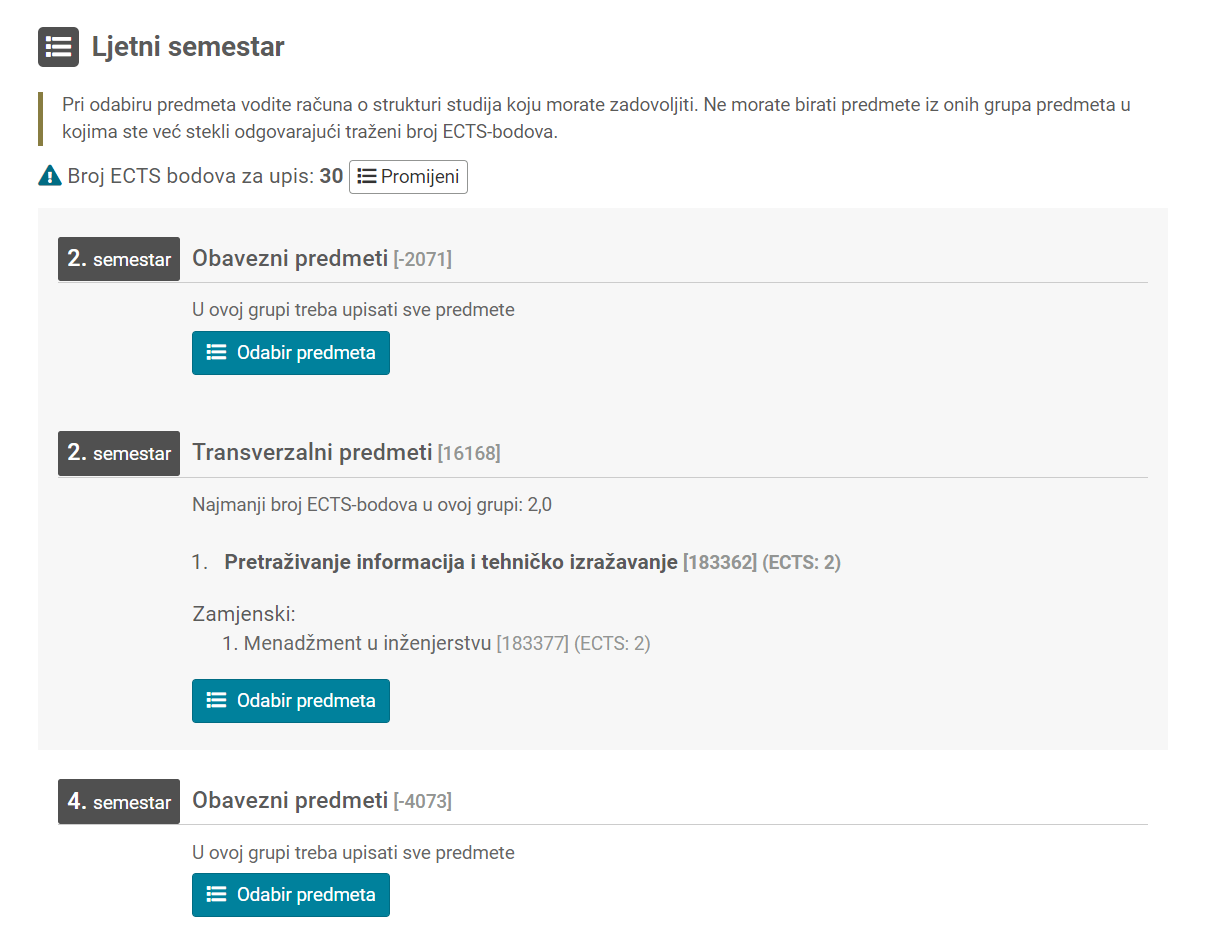
\includegraphics[scale=.6]{poboljsana/courses.png}}
          \centering
          \caption{Dio promijenjene stranice prikaza semestara u ljetnom semestru}
        \end{figure}
        
        \vspace{\baselineskip}
        \bigbreak
        Klikom na gumb \textit{Odabir predmeta} aplikacija korisnika vodi do stranice gdje bira predmete za upis i zamjenske predmete. Ovdje je naslov na početku stranice promijenjen da bolje opisuje čemu trenutačna stranica služi. Promjene obavljene u ovom dijelu aplikacije dodane su po zahtjevu studenata tijekom evaluacije. Na početak prikaza stranice  dodano je objašnjenje naziva \textit{Odabrani predmeti} i \textit{Zamjenski predmeti}. Kod odabranih (i zamjenskih) predmeta svi gumbi su prebačeni na početak retka, prije naziva predmeta, kako bi isti gumbi bili jedan ispod drugog i time njihovo korištenje bilo olakšano. S gumba je uklonjen tekst i ostavljene su samo ikonice koje dovoljno jasno prikazuju čemu služe. Ipak, napisane su i kratke upute na početku stranice koje objašnjavaju dodavanje predmeta i korištenje gumba pored naziva predmeta.
        
        Dodana je mogućnost izravnog prebacivanja predmeta iz odabranih u zamjenske i obrnuto pa studenti više ne moraju ukloniti predmet i ponovno ga dodati kada žele promijeniti listu na kojoj se on nalazi. Ovdje se predmet odmah uklanja s popisa na kojem je bio i pojavljuje se na kraju drugog popisa animacijom \textit{fadeInLeft} iz biblioteke animate.css. Pri dodavanju predmeta na listu prikazuje se animacije \textit{fadeInLeft} pri dodaji odnosno \textit{fadeOutRight} (iz biblioteke animate.css) za uklanjanje predmeta. Animacije su ovdje korištene da korisniku bude jasnije da se radnja dodavanja ili uklanjanja predmeta dogodila. Kada je akcija trenutačna, korisnik ne vidi radnju uklanjanja i dodavanja i to može u njemu pobuditi kratku zbunjenost. Iz istog su razloga dodane animacije \textit{slideOutUp} i \textit{slideOutDown} iz animate.css biblioteke za mijenjanje redoslijeda (prioriteta) u listama odabranih i zamjenskih predmeta.
        
        Boja gumba \textit{Dodaj} promijenjena je u primarnu plavu. Za bolji pregled stranice, ikone koje su korištene na gumbima \textit{Dodaj} i \textit{Zamj.} dodane su uz naziv liste predmeta. Na ovaj način korisnici ne moraju čitati svaki dio stranice, nego im je preko ikona jasno koji dijelovi su međusobno povezani.
        
        Gumb \textit{Detalji} pomaknut je pored gumba za dodavanje kako bi svaki gumb stajao na istom mjestu u retku. Klikom na taj gumb prikazuje se prozor s kratkim opisom predmeta. Na postojećoj aplikaciji tada se u novogeneriranom prozorčiću stvori i gumb za zatvaranje, a gumb \textit{Detalji} nestane. Ovo je promijenjeno tako da kada se otvori prozorčić, na mjestu gumba za otvaranje se stvori gumb za zatvaranje tako da dizajn ostane konzistentan.
        
        Naziv \textit{Ne drži se} kod predmeta koji se neće izvoditi u semestru promijenjen je u \textit{Ne održava se} zbog bolje jasnoće po zahtjevima studenata pri evaluaciji.
        
        Posljednji dodatak su info-oblačići (\textit{tooltips}) koji daju brzo i kratko objašnjenje kada korisnik obavi \textit{hover} akciju nad elementima \textit{Ograničenje}, \textit{Ne održava se} i \textit{Nije moguće upisati}. Ova mogućnost implementirana je pomoću biblioteke Effeckt.css.
        
        \begin{figure} [H]
          \fbox{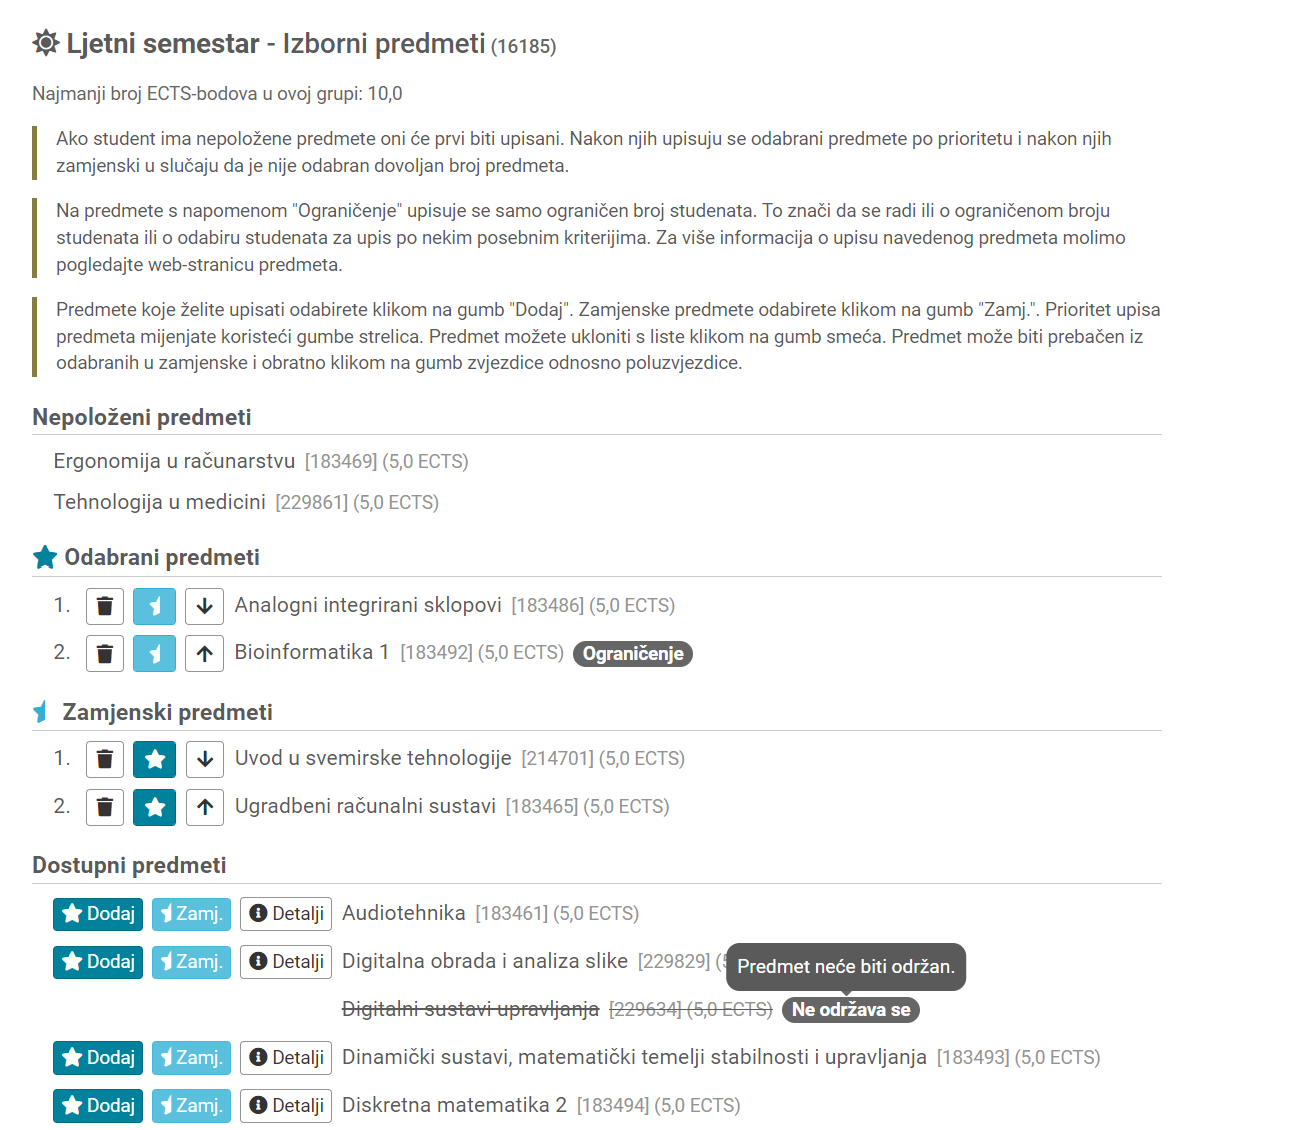
\includegraphics[scale=.5]{poboljsana/selectcourses.png}}
          \centering
          \caption{Prikaz dijela stranice za odabir izbornih predmeta}
        \end{figure}
        
        \noindent\textbf{Mentor/ica}
        
        U listi odabranih mentora, s gumba za mijenjanje poretka prioriteta uklonjen je tekst i ostavljene su samo ikonice. Ti su gumbi prebačeni na početak retka kako bi isti gumbi bili uredno poredani jedan ispod drugog te su na njih dodane animacije \textit{slideOutUp} i \textit{slideOutDown} pri promjeni redoslijeda prioriteta mentora. Ovo je dodano zbog boljeg uočavanja promjene pri odabiru gumba. Stranica ima polje za pretraživanje koje podržava upis imena, titule ili kratice zavoda mentora. U listi dostupnih mentora gumb \textit{Info} za prikaz više detalja o mentoru prebačen je na početak retka nakon gumba \textit{Odabir} kako bi se svi isti gumbi nalazili izravno jedan ispod drugog. Boja gumba za biranje mentora promijenjena je u plavu. Osim animacije pri promjeni redoslijeda predmeta, dodane su animacije \textit{fadeInLeft} pri odabiru mentora te \textit{fadeOutRight} pri uklanjanju mentora s popisa odabranih mentora.
        
        \begin{figure} [H]
          \fbox{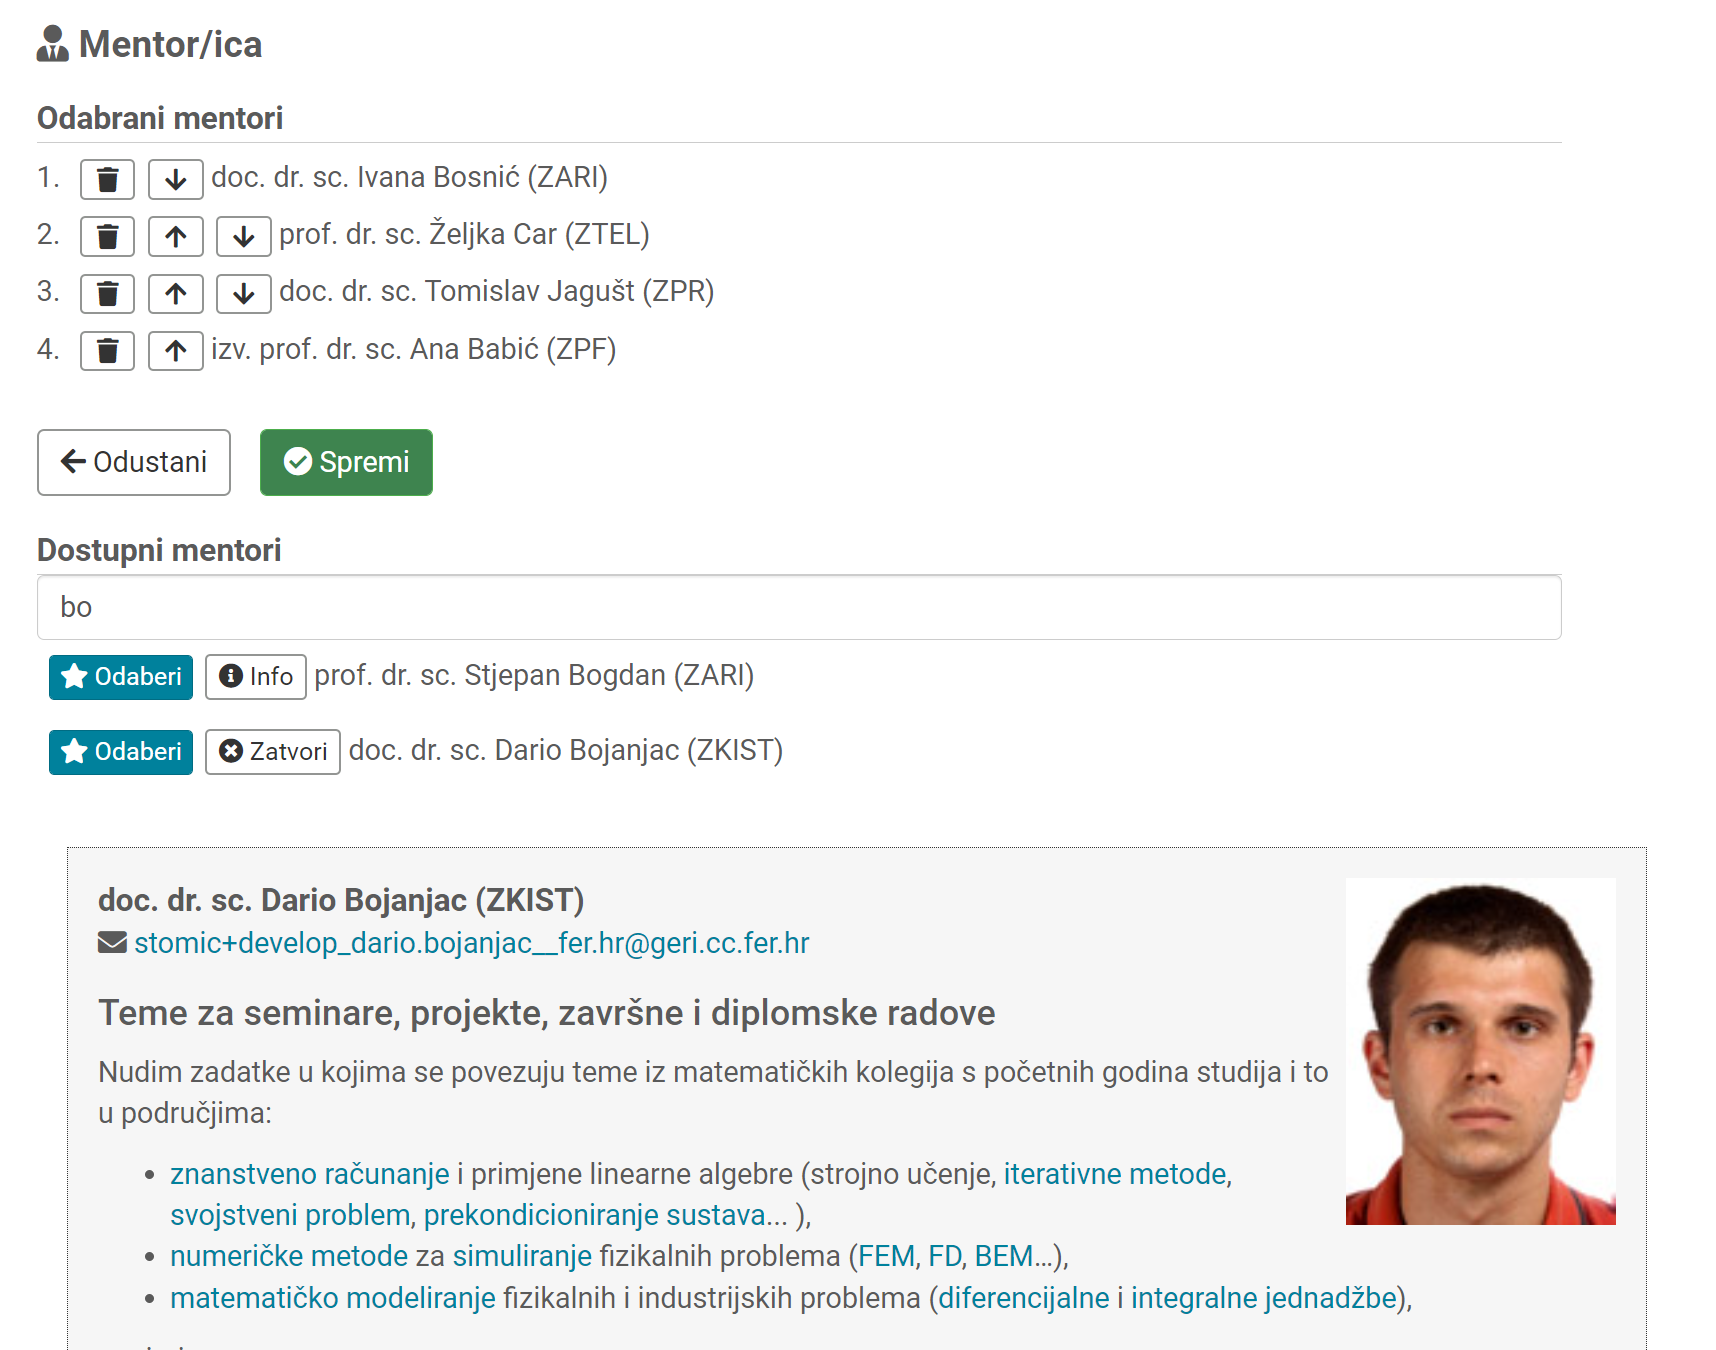
\includegraphics[scale=.6]{poboljsana/mentor.png}}
          \centering
          \caption{Promijenjena stranica odabira mentora}
        \end{figure}
        
        \noindent\textbf{Plaćanje}
        
        Na stranci plaćanja elementi drugog stupca približeni su svojim oznakama i uklonjena je oznaka \textit{Računi} jer je jasno da se u tablici radi o računima.
        
        \begin{figure} [H]
          \fbox{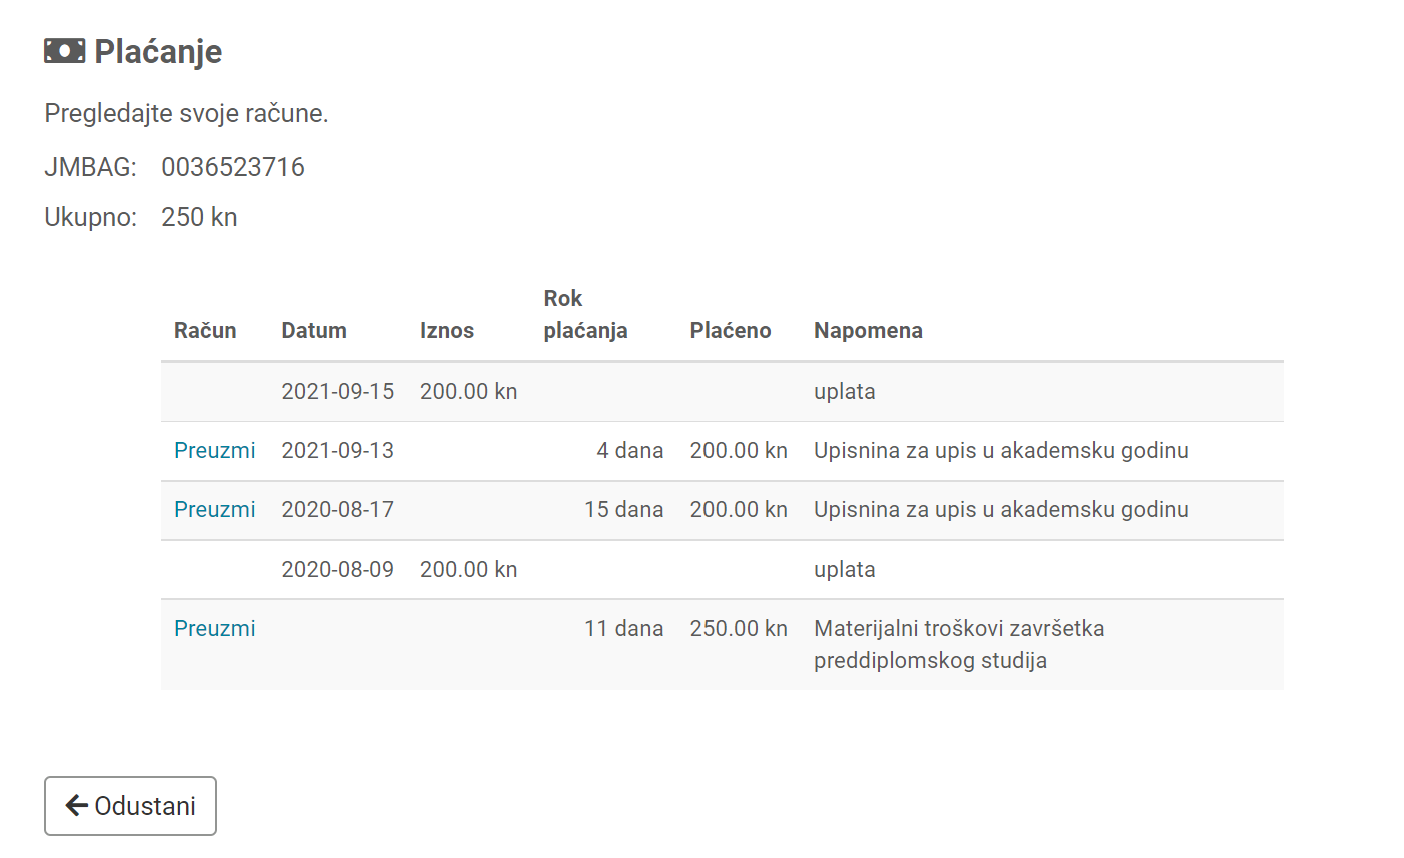
\includegraphics[scale=.6]{poboljsana/payment.png}}
          \centering
          \caption{Promijenjena stranica računa}
        \end{figure}
        
        \vspace{\baselineskip}
        \bigbreak
        \noindent\textbf{Simulacija}
        
        Svi studenti koji su sudjelovali u procjeni postojeće aplikacije imali su primjedbe na zasićenost informacijama stranice simulacije. Problem je riješen korištenjem ikonica pored svakog predmeta i legende tih ikonica na početku stranice. Na ovaj način, kratko se objašnjenje više ne nalazi ispod naziva svakog od predmeta, već je ono preneseno preko korištenih ikonica. Ovdje je primijenjen Gestalt zakon iskustva po kojemu određene tehnike ili elementi imaju univerzalna značenja. Koriste se tri vrste ikonica čime njihovo prepoznavanje ne ovisi samo o boji pa je time prilagođeno osobama s poteškoćama u prepoznavanju boja. Osim nepreglednosti stranice, studenti su tijekom procjene napomenuli kako nije dovoljno jasno što znači mogućnost preklapanja predmeta. Zbog toga je promijenjen opis preklapanja za bolje razumijevanje mogućnosti. Opis je i prebačen s kraja na početak stranice.

        \begin{figure} [H]
          \fbox{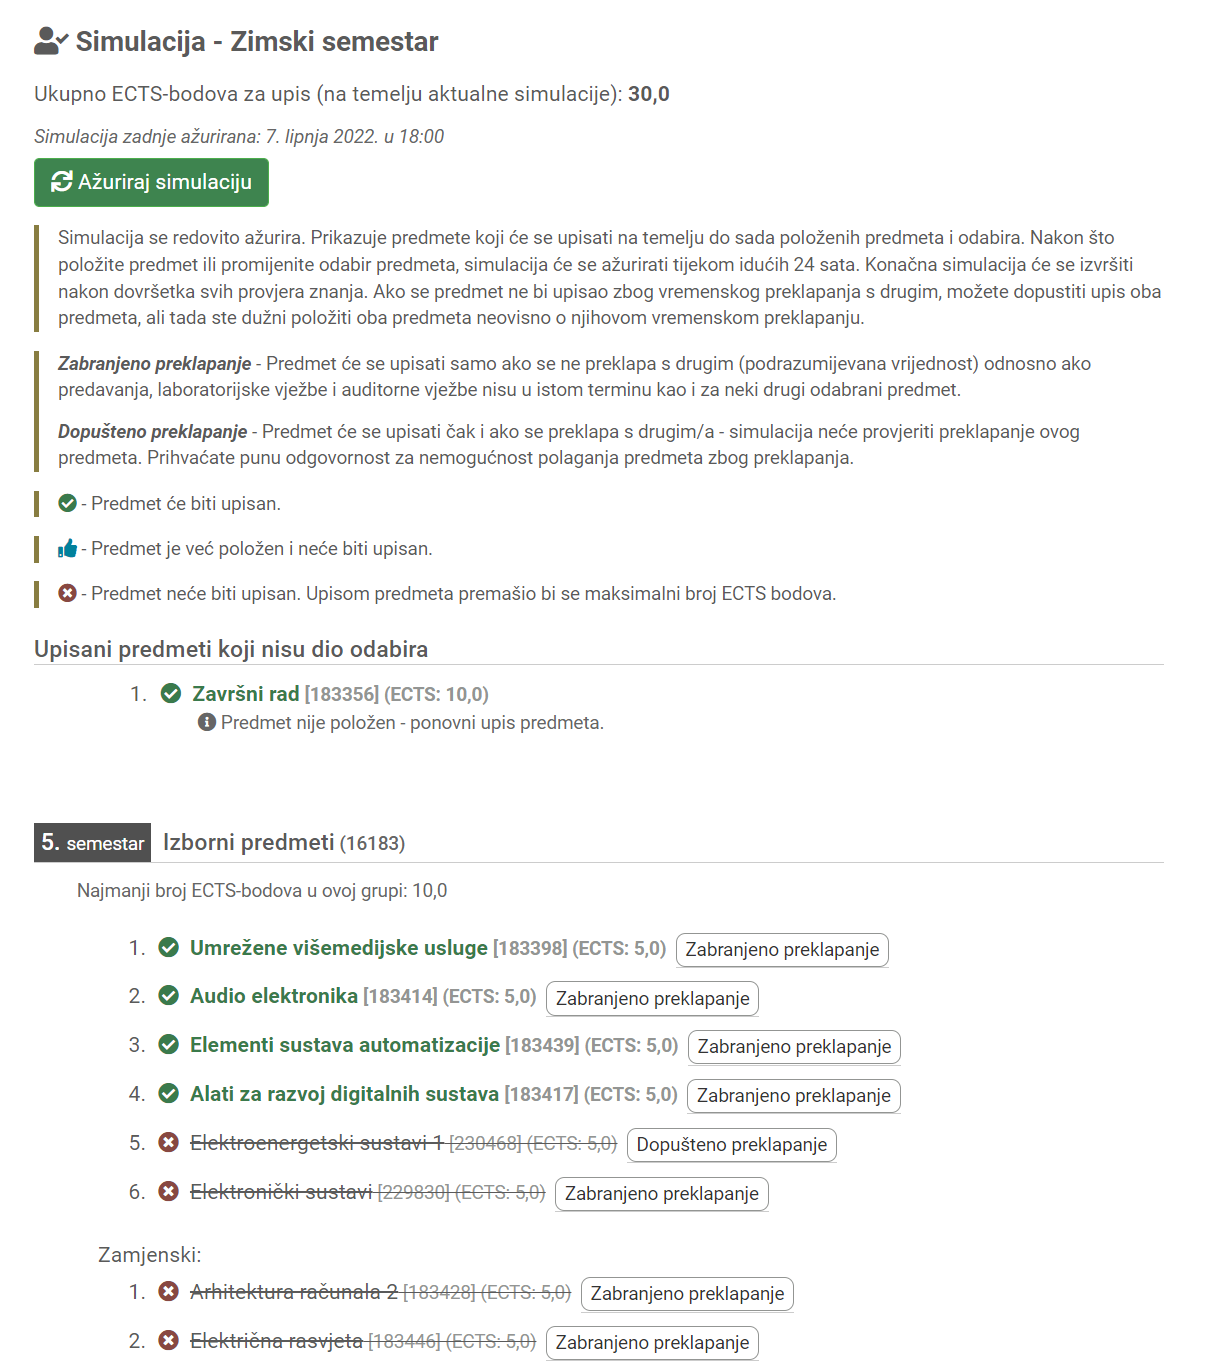
\includegraphics[scale=.6]{poboljsana/simulation.png}}
          \centering
          \caption{Dio promijenjene stranice simulacije}
        \end{figure}

        \subsection{Evaluacija poboljšanog dizajna}
        Nakon što su obavljene neke promjene nad starim dizajnom, isti studenti su evaluirali poboljšani dizajn te dali svoje komentare i ocjene.
        
        Stranica \textbf{biranja studijskog programa} dobila je pohvale zbog malih promjena koje su pridonijele njezinom jednostavnijem izgledu. Fokus je stavljen isključivo na biranje jednog programa.
        
        Na ovom dizajnu svi su studenti primijetili opciju promjene ECTS-bodova na stranici \textbf{prikaza semestara}. Komentari na novi izgled popisa semestara i dalje su sadržavali primjedbe na prikaz semestara koje su studenti već dovršili.
        
        Studenti, koji su primijetili promjene u prikazu odabranih predmeta na stranici sa semestrima, potvrdili su kako poboljšani izgled stavlja veću važnost na odabrane predmete i ističe ih.
        
        \textbf{Stranica odabira predmeta i zamjenskih predmeta} dobila je najviše pozitivnih komentara. Studentima se opcija prebacivanja odabranih predmeta izravno u zamjenske i obrnuto učinila jako korisnom. Kako se u poboljšanom dizajnu gumbi na svim popisima (odabrani, zamjenski, dostupni) nalaze u istom stupcu jedni ispod drugog, studentima je bilo puno lakše odabirati gumbe. Ovo se pogotovo odnosi na mijenjanje redoslijeda željenih predmeta koje je u ovom dizajnu popraćeno animacijama. Jedina primjedba bila je na biranje predmeta, točnije na naporan posao traženja željenog predmeta u listi dostupnih predmeta. Prosječna ocjena iskustva studenata pri korištenju ove stranice je \textbf{4.2/5}.
        
        \begin{figure} [H]
          \fbox{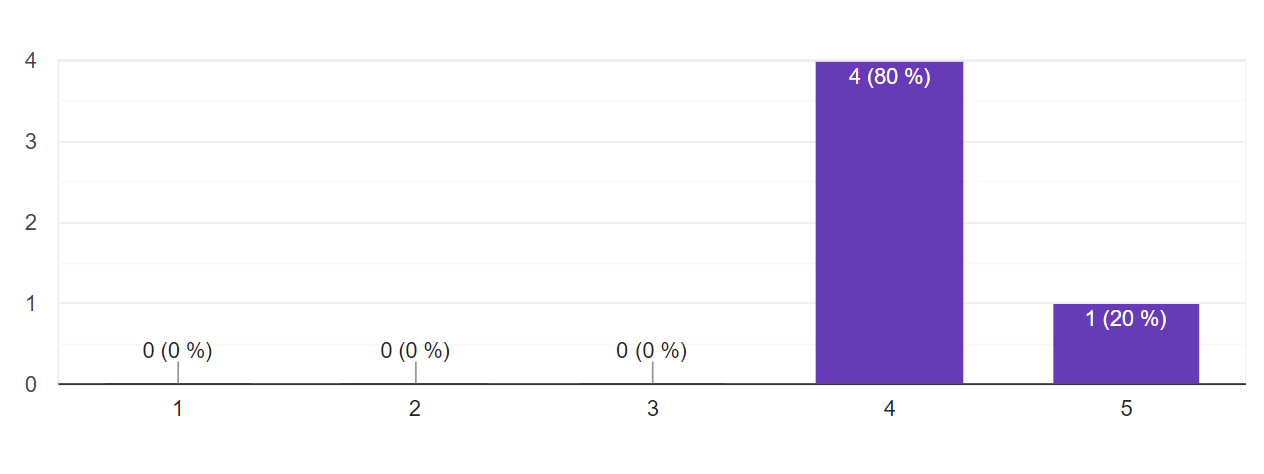
\includegraphics[scale=.6]{poboljsana/courses_ocjena.png}}
          \centering
          \caption{Ocjene korisničkog iskustva poboljšanog dizajna stranice odabira predmeta i prikaza semestara}
        \end{figure}
        
        \textbf{Stranica plaćanja} je i s ovim dizajnom dobila kritike. Jedina, ali ujedno i pozitivna promjena, bila je centriranje tablice računa. Svaki je od pet studenata i dalje isticao nejasnoću tablice. Prosječna ocjena iskustva studenata pri korištenju ove stranice je \textbf{2/5}.
        
        \begin{figure} [H]
          \fbox{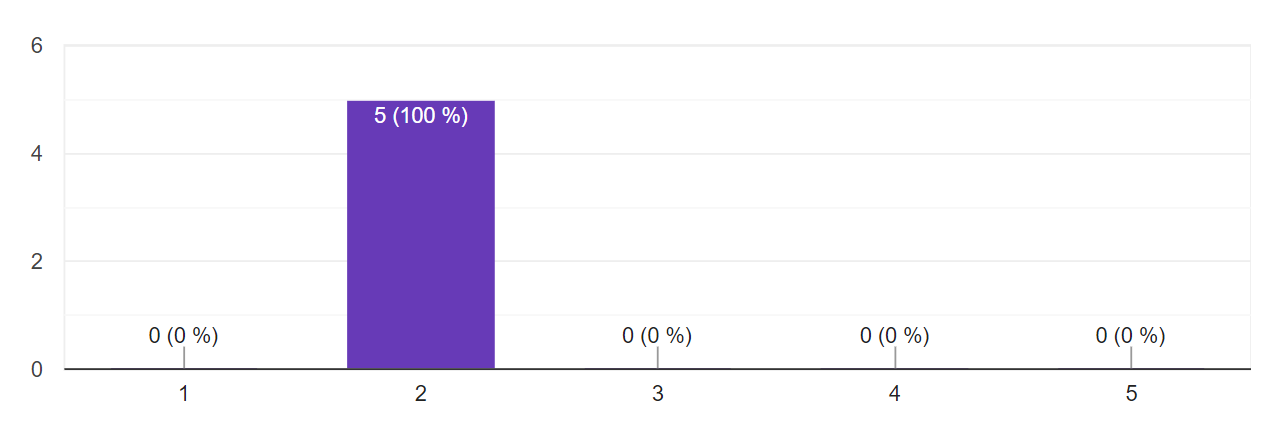
\includegraphics[scale=.6]{poboljsana/placanje_ocjena.png}}
          \centering
          \caption{Ocjene korisničkog iskustva poboljšanog dizajna stranice plaćanja}
        \end{figure}
        
        U \textbf{simulaciji} su svi studenti komentirali kako s novijim izgledom zbog uporabe legende ikonica ima manje teksta koji odvlači pozornost i osoba brže uočava koji predmeti će joj biti upisani. Također zbog poboljšanog opisa značenja termina \textit{Dopušteno/Zabranjeno preklapanje} studenti su znali što mogu očekivati kada odaberu jednu od tih dviju opcija.
        
        Nakon evaluacije pojedinačnih stranica studenti su ocjenjivali svoje ukupno iskustvo korištenja aplikacije. Prosječna ocjena iskustva studenata pri korištenju poboljšane aplikacije je \textbf{4/5}.
        
        \begin{figure} [H]
          \fbox{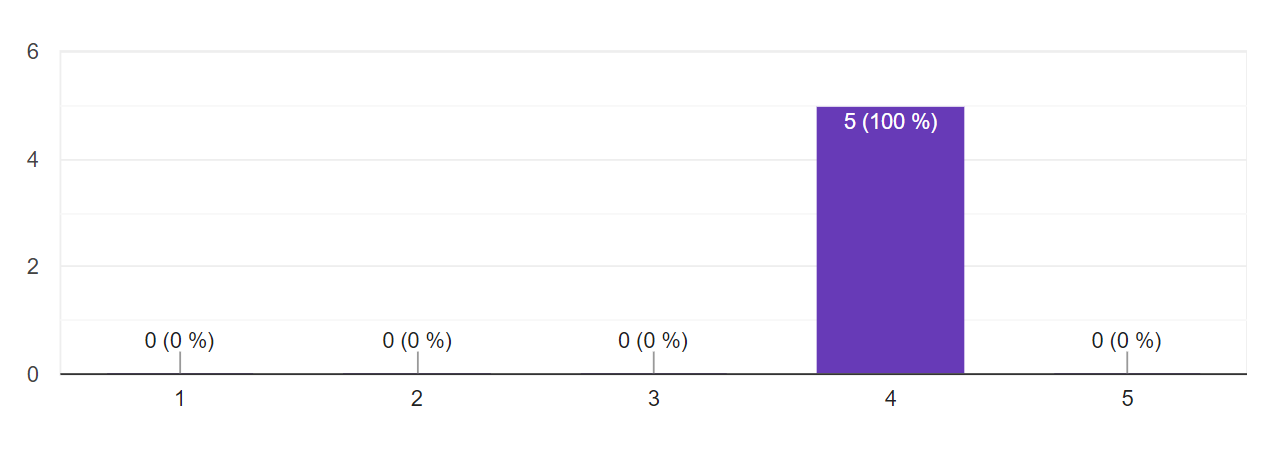
\includegraphics[scale=.6]{poboljsana/overall.png}}
          \centering
          \caption{Ocjene korisničkog iskustva korištenja aplikacije poboljšanog dizajna}
        \end{figure}
        

        
\chapter{Novi dizajn modula}
    \section{Opis novog dizajna}
    U novom dizajnu modula, odnosi između stranica ostali su jednaki kao na trenutačno postojećoj verziji. Korisnik se po modulu kreće \textbf{odabirom kartica} na vrhu stranice. Ovime se korisniku daje \textbf{fleksibilnost} da u bilo kojem trenutku može doći na neki drugi korak upisa, a ne vraćati se na početnu stranicu. Ovim dizajnom primijenjeno je \textbf{načelo pojavljivanja} Gestalt psihologije. Ono govori kako se slični objekti prepoznavaju kao jedna cjelina umjesto kao skup dijelova. Kartice se razlikuju ikonicama i neutralne su plave boje. Nijansa plave odgovara onoj koja se koristi na ostatku web-stranica Fakulteta. U slučaju da korisniku nije jasno što koja ikonica na karticama predstavlja, intuitivno će pozicionirati miš na karticu koja ga zanima. U tom trenutku kartica će se animirano proširiti i pojavit će se naziv koji bi inače pisao kada je kartica aktivna. Ovo je implementirano kao mogućnost u svakom koraku upisa.
    
    \begin{figure} [H]
      \fbox{
\includegraphics[scale=.6]{nova/hover.png}}
      \centering
      \caption{Prikaz \textit{hover} funkcionalnosti na kartici Mentora/ice}
    \end{figure}
    
    Kod promjene stranica koristi se animacija vertikalne translacije prema gore pri izlazu sa stranice te onda prema dolje pri ulazu na novu stranicu. Za ovo je korištena komponenta \textit{Transition}. Opširnije objašnjenje nalazi se u poglavlju 5, \textit{Izrada poboljšanog i novog modula}.
    
    Pri učitavanju aplikacije korisnik je poslan na zadnju karticu s nazivom \textit{Predaj} i ikonicom zelene kvačice ako prijava nije predana odnosno zelenog lokota ako prijava jest predana. To je jedina kartica zelene boje i jedina na kojoj se osim ikonice nalazi i tekst čak i kada nije aktivna. Ovo je napravljeno zbog odvajanja posljednje kartice od ostalih tijekom cijelog procesa upisa. Ostale kartice na sebi imaju isključivo ikonice i tekst se pojavi samo onda kada je ta kartica aktivna.
    
    Na kartici \textit{Predaj} nalazi se sažetak korisnikovog procesa upisa u godinu i gumb za predaju. Tamo studenti mogu vidjeti koji koraci upisa su riješeni, a koji još trebaju biti obavljeni. Za obavljen korak prikazana je \textbf{ikonica zelene kvačice} i naveden je odabir studenta. Koraci koje korisnik još treba proći imaju \textbf{ikonicu crvenog križića} i poruku kako odabir za taj korak još nije donesen. Za prikaz odabranih predmeta po semestru ponovno je korištena biblioteka animate.css i njezine animacije \textit{fadeInDown} i \textit{fadeOutUp}.
    
    Korak za predaju prijave crtom je odvojen od sažetka odabira po koracima zbog boljeg isticanja. Pri učitavanju stranice na gumbu prijave ponovno je dodana animacija \textit{fadeInLeft} iz biblioteke animate.css iz istog razloga kao i u poboljšanom dizajnu, zbog jačeg isticanja. U slučaju da prijava ne može biti izvršena, u dijelu stranice nakon crte bit će navedeni razlozi nemogućnosti zaključavanja prijave. Font korišten u cijeloj aplikaciji je \textit{Open Sans} i uzet je s repozitorija Google Fonts\footnote{https://fonts.google.com/}.
    
    \begin{figure} [H]
      \fbox{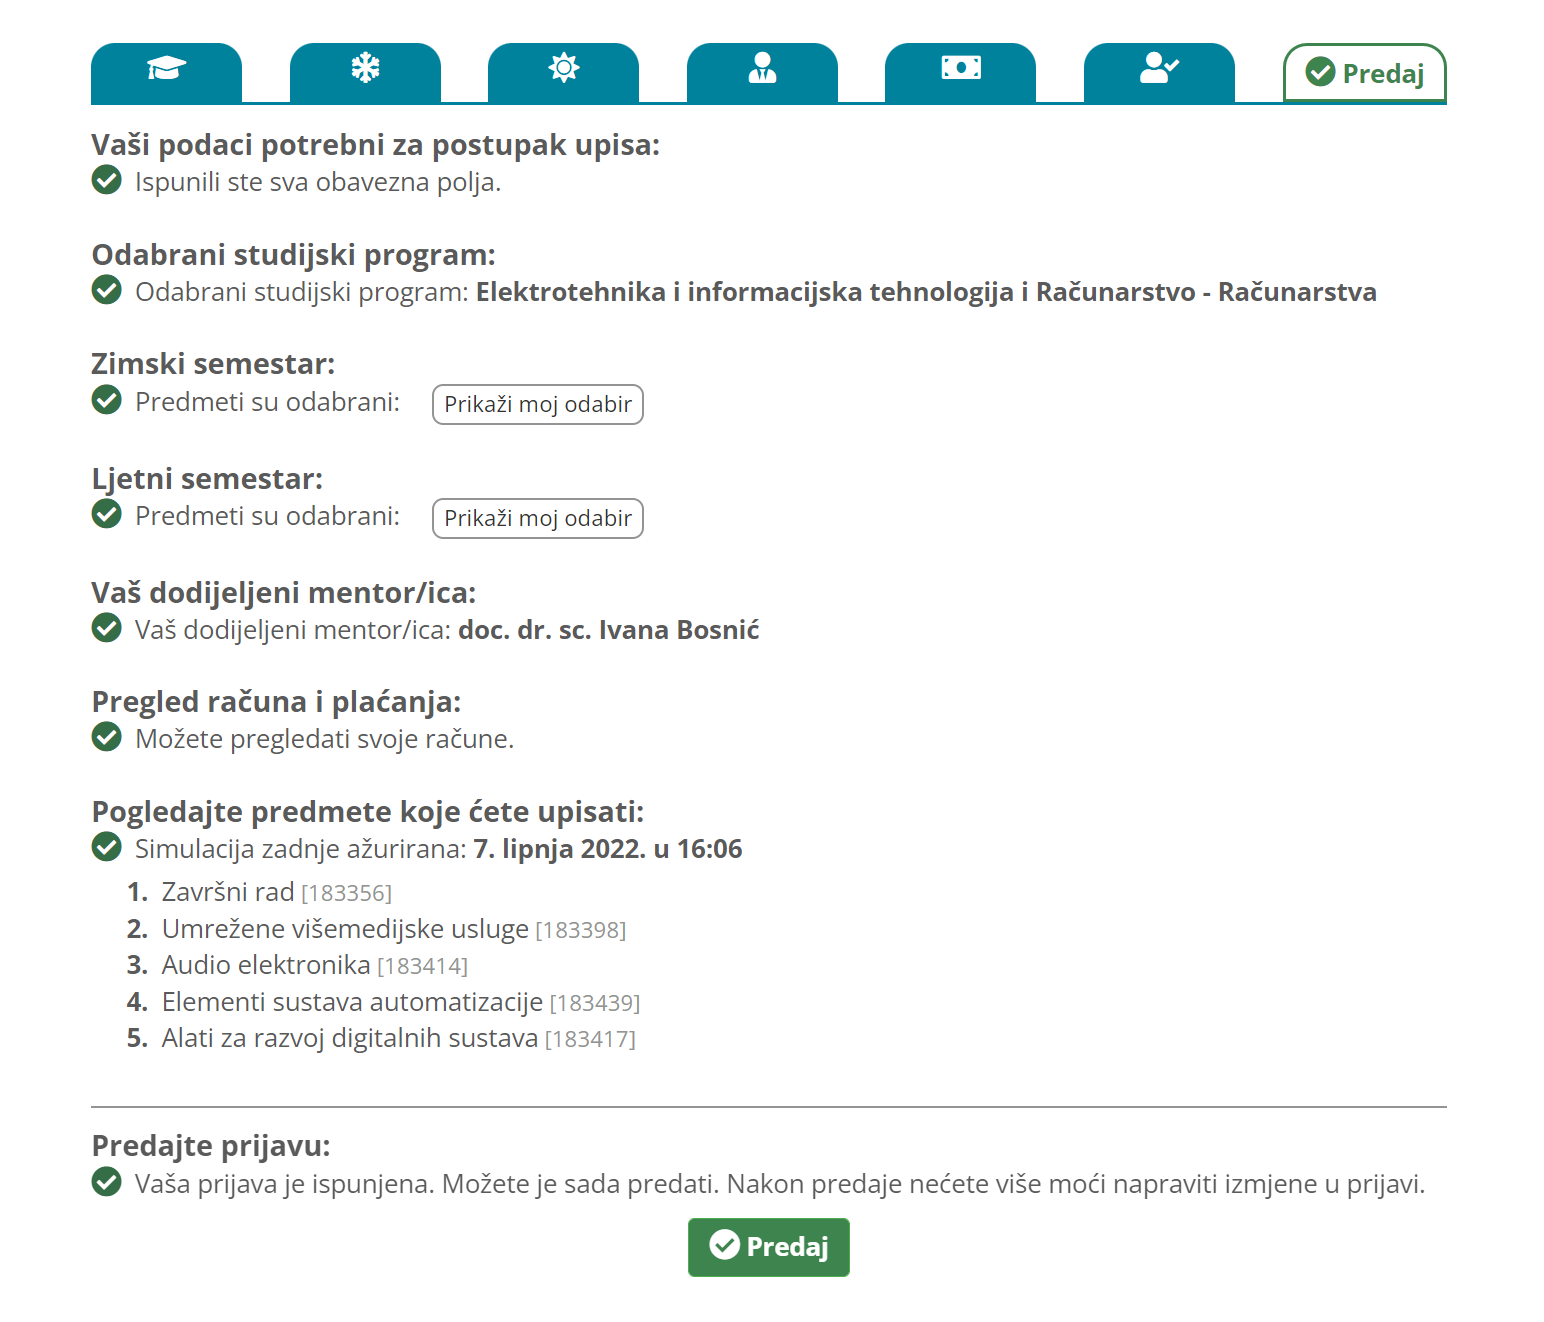
\includegraphics[scale=.6]{nova/index_spremno.png}}
      \centering
      \caption{Početna stranica - prijava spremna za predaju}
    \end{figure}
    
    \begin{figure} [H]
      \fbox{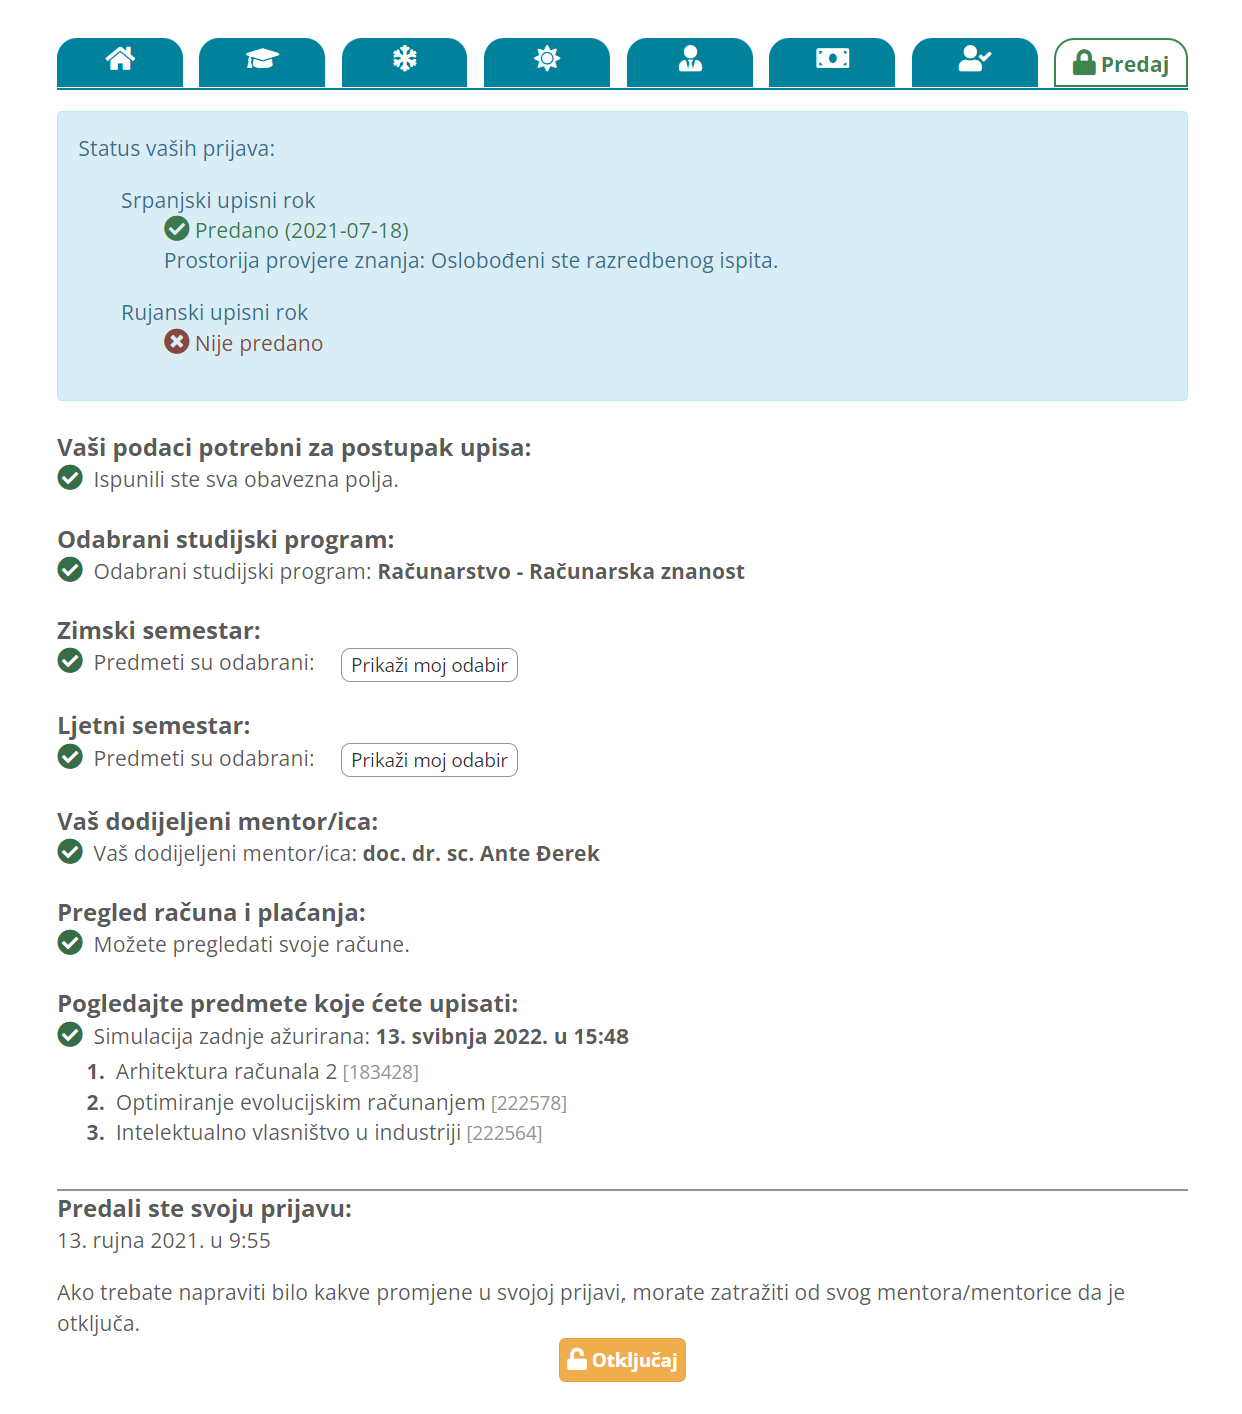
\includegraphics[scale=.5]{nova/index_predano.png}}
      \centering
      \caption{Početna stranica predanog upisa na diplomski studij}
    \end{figure}
    
    Aplikacija novog dizajna ima mogućnost \textbf{višejezičnog} prikaza odnosno prikaza sadržaja na hrvatskom i engleskom jeziku. Uz to, aplikacija je prilagođena i za uređaje manjih dimenzija uporabom \textbf{responzivnosti}. 
    
    \begin{figure} [H]
      \fbox{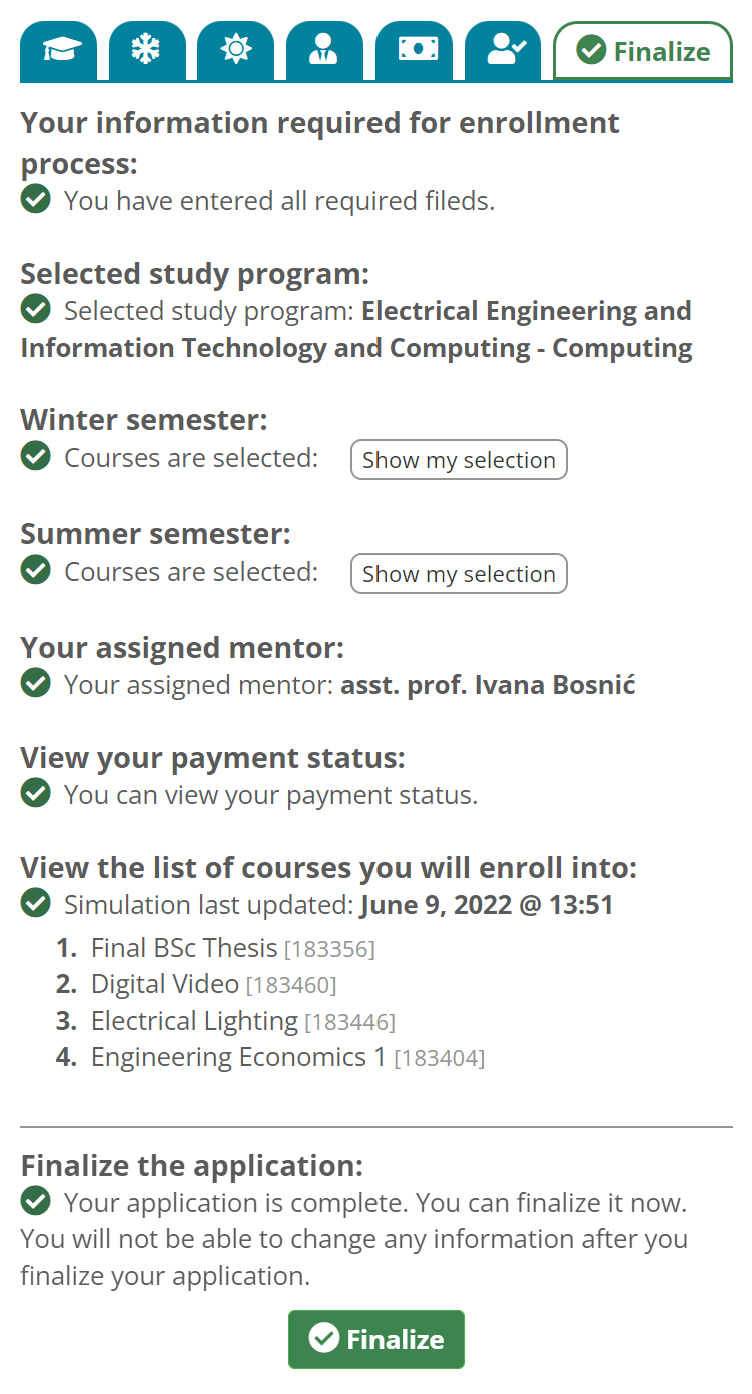
\includegraphics[scale=.45]{nova/responzivnost.png}}
      \centering
      \caption{Prikaz responzivnosti i dvojezičnosti aplikacije}
    \end{figure}
    
    
    
    \noindent\textbf{Vaše informacije}
    
    Prvi korak i prva kartica odnose se na upis podataka o studentu. Ovo se obavlja samo ako se radi u upisu na prvu godinu studija. U suprotnom, kartica korisniku nije vidljiva. U ovom koraku student ispunjava obrazac o osobnim podacima, podacima vezanim uz dosadašnje obrazovanje, obrazovanje svojih roditelja, mjestu prebivališta i boravišta te ostale informacije potrebne za upis.
    %\linebreak \linebreak
    \vspace{\baselineskip}
    %\bigbreak
    
    \noindent\textbf{Studijski program}
    
    Sljedeći korak je odabir studijskog programa. Korisniku je na stranici prikazan popis ponuđenih studijskih programa za upis. Kretanjem mišem po izborima, pozadina programa nad kojim je miš pozicioniran poprimi svjetlo sivu pozadinu zbog boljeg uočavanja na kojem odabiru se korisnik trenutno nalazi. Ovo se ne događa odmah, već ima animaciju \textit{ease-out} povezanu s tom akcijom. U sredini na kraju stranice nalazi se zeleni gumb za spremanje odabira \textit{Spremi} s bijelom ikonicom kvačice. Odabrani studijski program ističe se od ostalih svojom plavom pozadinom. 
    
    \begin{figure} [H]
      \fbox{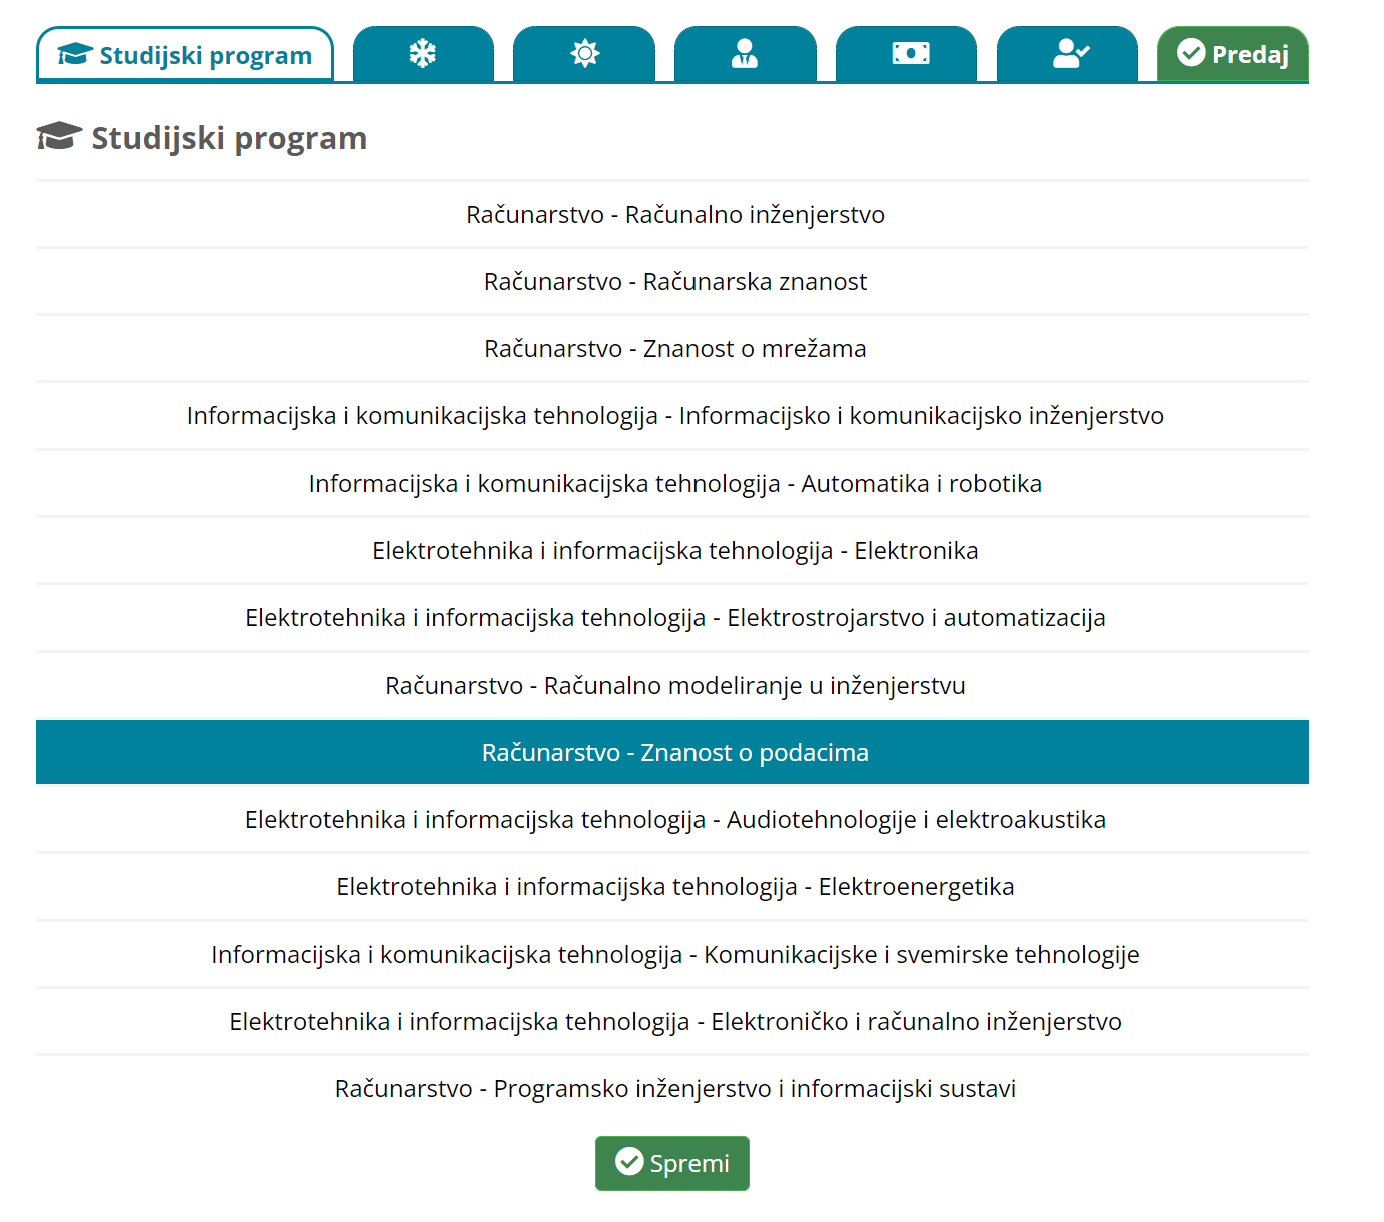
\includegraphics[scale=.6]{nova/studijski_program.png}}
      \centering
      \caption{Prikaz odabira studijskog programa}
           % \caption{Prikaz odabira studijskog programa}

    \end{figure}
    
    \noindent\textbf{Odabir predmeta}
    
    Nakon odabira studijskog programa student može prijeći na odabir predmeta za upis u zimskom i ljetnom semestru. Na početku stranice za odabir semestra nalazi se poruka o tome da studenti sami paze u kojoj grupi predmeta u kojem semestru trebaju upisivati predmete. Studenti su pri procjeni aplikacije primijetili prikaz grupa za 2. semestar iako su položili sve predmete tog semestra. Semestar se prikazuje zbog prevencije pogrešaka pri upisu zbog mogućih promjena u sustavu. Može se dogoditi da dođe do izmjena predmeta u nekoj kategoriji. Ako se kategorija ne prikazuje, student neće moći upisati potreban predmet i upis neće biti ispravan zbog pogreške aplikacije. Iz ovog razloga prikazuju se sve kategorije i ostavljeno je na studentima da sami paze što je potrebno upisati.
    
    Nakon poruke nalazi se opcija promjene broja ECTS-bodova za upis koji je izvorno uvijek postavljen na 30. Klikom na gumb \textit{Promijeni} aplikacija nas vodi na novu stranicu za promjenu broja bodova. Stranica je sasvim jasna korisnicima, stoga nije bila ponovno mijenjana te izgleda kao ona u poboljšanom dizajnu. Iznimka je gumb \textit{Spremi} koji se sada nalazi na sredini stranice te gumb \textit{Odustani} više nije uopće prikazan. Na stranici biranja semestra može se vratiti klikom na aktivnu karticu. Ispod toga nalazi se gumb za prikaz svih predmeta. Kada ga se klikne prikažu se i grupe predmeta u kojima studenti ne trebaju upisati nijedan predmet. To su vještine i predmeti za iznimno uspješne studente.
    
    Nakon toga slijedi popis grupa predmeta po semestrima. Naslovi koji uključuju semestar i naziv grupe predmeta nalaze se na sredini stranice jedan ispod drugog. Za svaku grupu naveden je broj bodova koji je potrebno upisati i gumb za odabir predmeta koji nas vodi na biranje predmeta za upis. Gumb je bijele boje i ima plavi obrub. Ovako je dizajniran kako se ne bi poistovjećivao s karticama zbog sličnog izgleda. Hijerarhija je takva da su kartice smatrane primarnim gumbima i iz tog razloga imaju (plavu) boju za pozadinu. Gumb \textit{Odabir predmeta} je sekundarni gumb i zbog toga ima klasičnu bijelu pozadinu i malo je naglašen obrubom i tekstom plave boje \cite{tips}. Ispod gumba prikazan je popis odabranih i zamjenskih predmeta u toj kategoriji. Semestri su međusobno odvojeni na način da svaki drugi ima svijetlo sivu pozadinu. Ovo je učinjeno zbog bolje preglednosti i razdvajanja semestara. Bolja opcija bilo bi korištenje harmonike \textit{(accordion)}. Tada bi imali tri harmonike i pod jednom harmonikom nalazile bi se sve grupe za taj semestar. Studentima bi početno bile prikazane tri harmonike i rastvarali bi samo onu za semestar koji upisuju. Time bi se puno poboljšala preglednost stranice. Međutim, ovo nije bilo moguće implementirati zbog načina pohranjivanja podataka u bazu koju aplikacija koristi. Nazivi odabranih predmeta su podebljani i ID predmeta nalazi se u uglatim zagradama nakon naziva. Nakon ID-a slijedi broj ECTS-bodova predmeta u običnim zagradama. Za zamjenske predmete korištena je normalna debljina teksta i popis je uvučen udesno s obzirom na popis odabranih predmeta. 

    \begin{figure} [H]
      \fbox{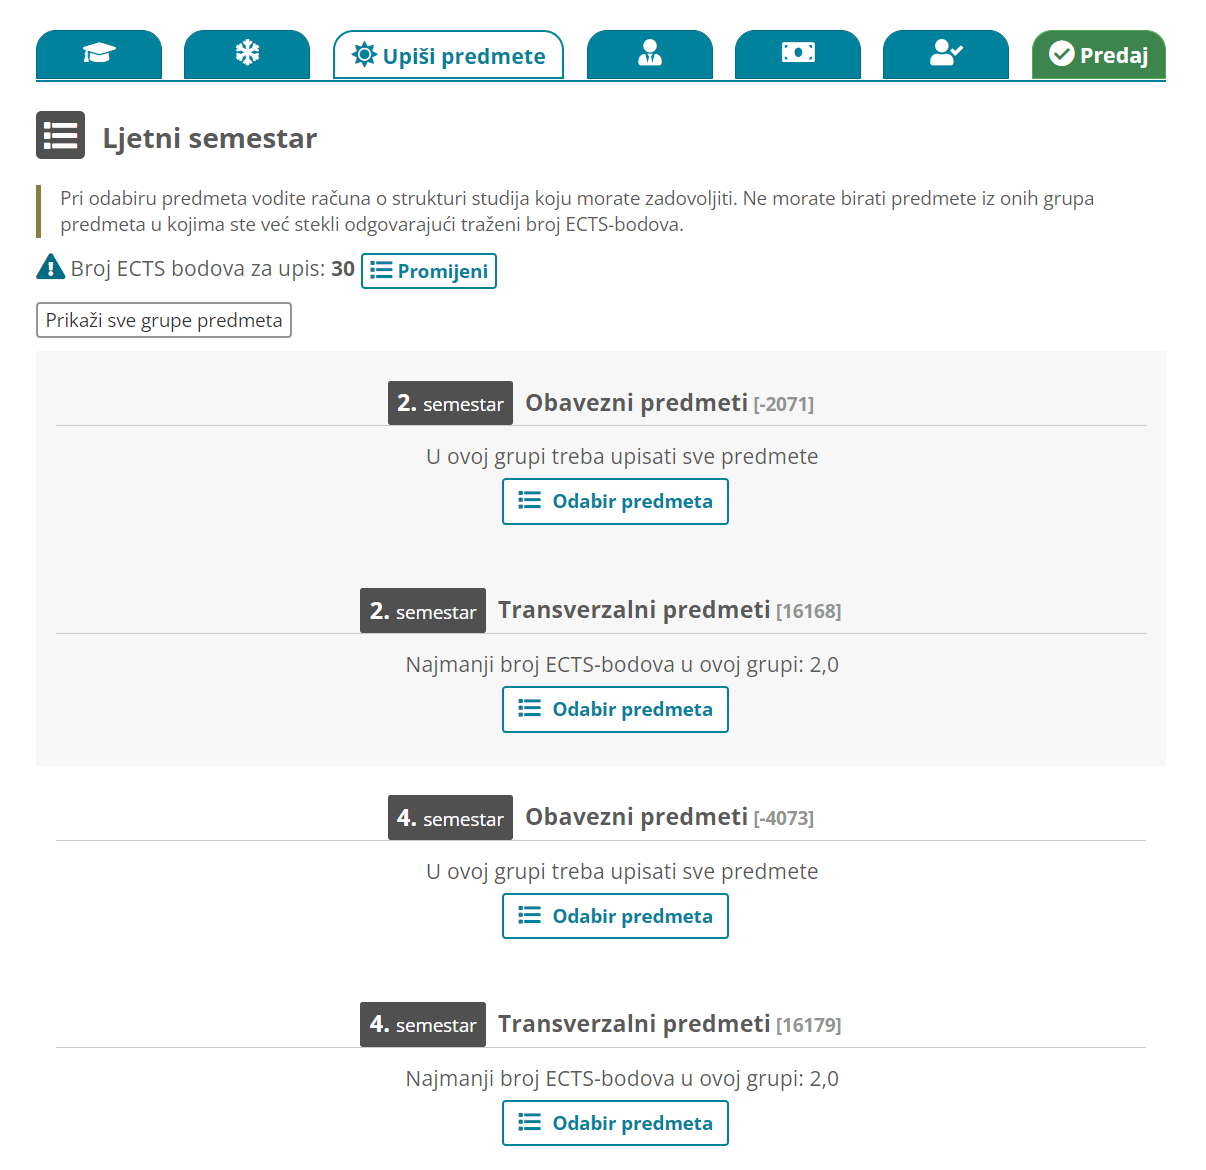
\includegraphics[scale=.6]{nova/courses_1.png}}
      \centering
      \caption{Prvi dio stranice prikaza semestara}
    \end{figure}
    
    \begin{figure} [H]
      \fbox{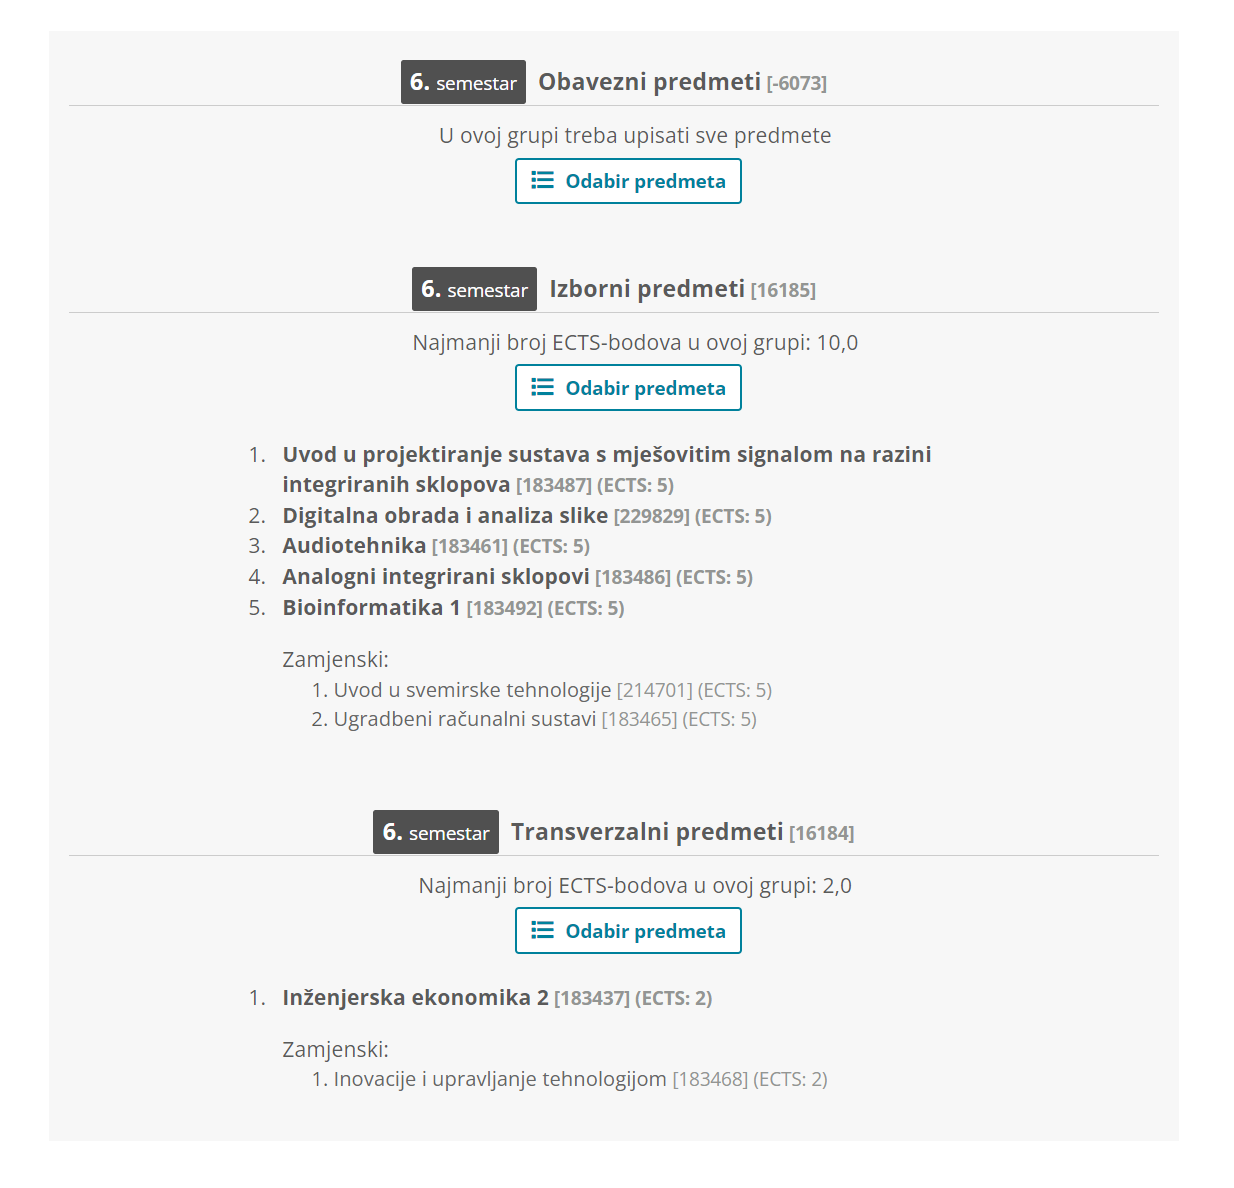
\includegraphics[scale=.6]{nova/courses_2.png}}
      \centering
      \caption{Drugi dio stranice prikaza semestara}
    \end{figure}
    
    Klikom na gumb \textit{Odabir predmeta} za određenu grupu predmeta aplikacija korisnika vodi na stranicu gdje je moguće birati predmete za upis i zamjenske predmete. Za svaki odabrani i zamjenski predmet korisnik ima mogućnost promjene redoslijeda predmeta na popisu odnosno prioriteta upisa predmeta. Ova akcija popraćena je animacijama \textit{slideOutUp} i \textit{slideOutDown} jer kao i u poboljšanom dizajnu, daje bolju povratnu informaciju korisniku. Predmet može biti uklonjen s popisa klikom na gumb s ikonom kante za smeće. Pri dodavanju i uklanjanju predmeta prikazuju se animacije \textit{fadeInLeft} odnosno \textit{fadeOutRight} iz biblioteke animate.css. Predmet može biti prebačen iz popisa odabranih u popis zamjenskih i obrnuto klikom na gumb s ikonicom zvjezdice odnosno poluzvjezdice. Ovom akcijom predmet je uklonjen s popisa na kojem se nalazio i dodan na kraj drugog popisa. Radnja je popraćena animacijom \textit{fadeInLeft} iz biblioteke animate.css. Za oznake \textit{Ograničenje}, \textit{Ne održava se} i \textit{Nije moguće upisati} aktivira se info-oblačić kada je miš pozicioniran na neku od njih i korisnik vidi kratko objašnjenje značenja ovih termina. Ovaj element nalazi se u biblioteci Effeckt.css.
    
    Gumb za spremanje korisnikovog odabira nalazi se izravno ispod popisa željenih predmeta. Ovime je uklonjeno bespotrebno listanje do kraja stranice kako bi odabir bio spremljen. Iza gumba \textit{Spremi} nalazi se polje za pretraživanje. Ondje korisnik može pretraživati predmete po njihovim nazivima na hrvatskom i engleskom jeziku ili ID-u predmeta te ih time brže dodavati u liste željenih predmeta.
    
    \begin{figure} [H]
      \fbox{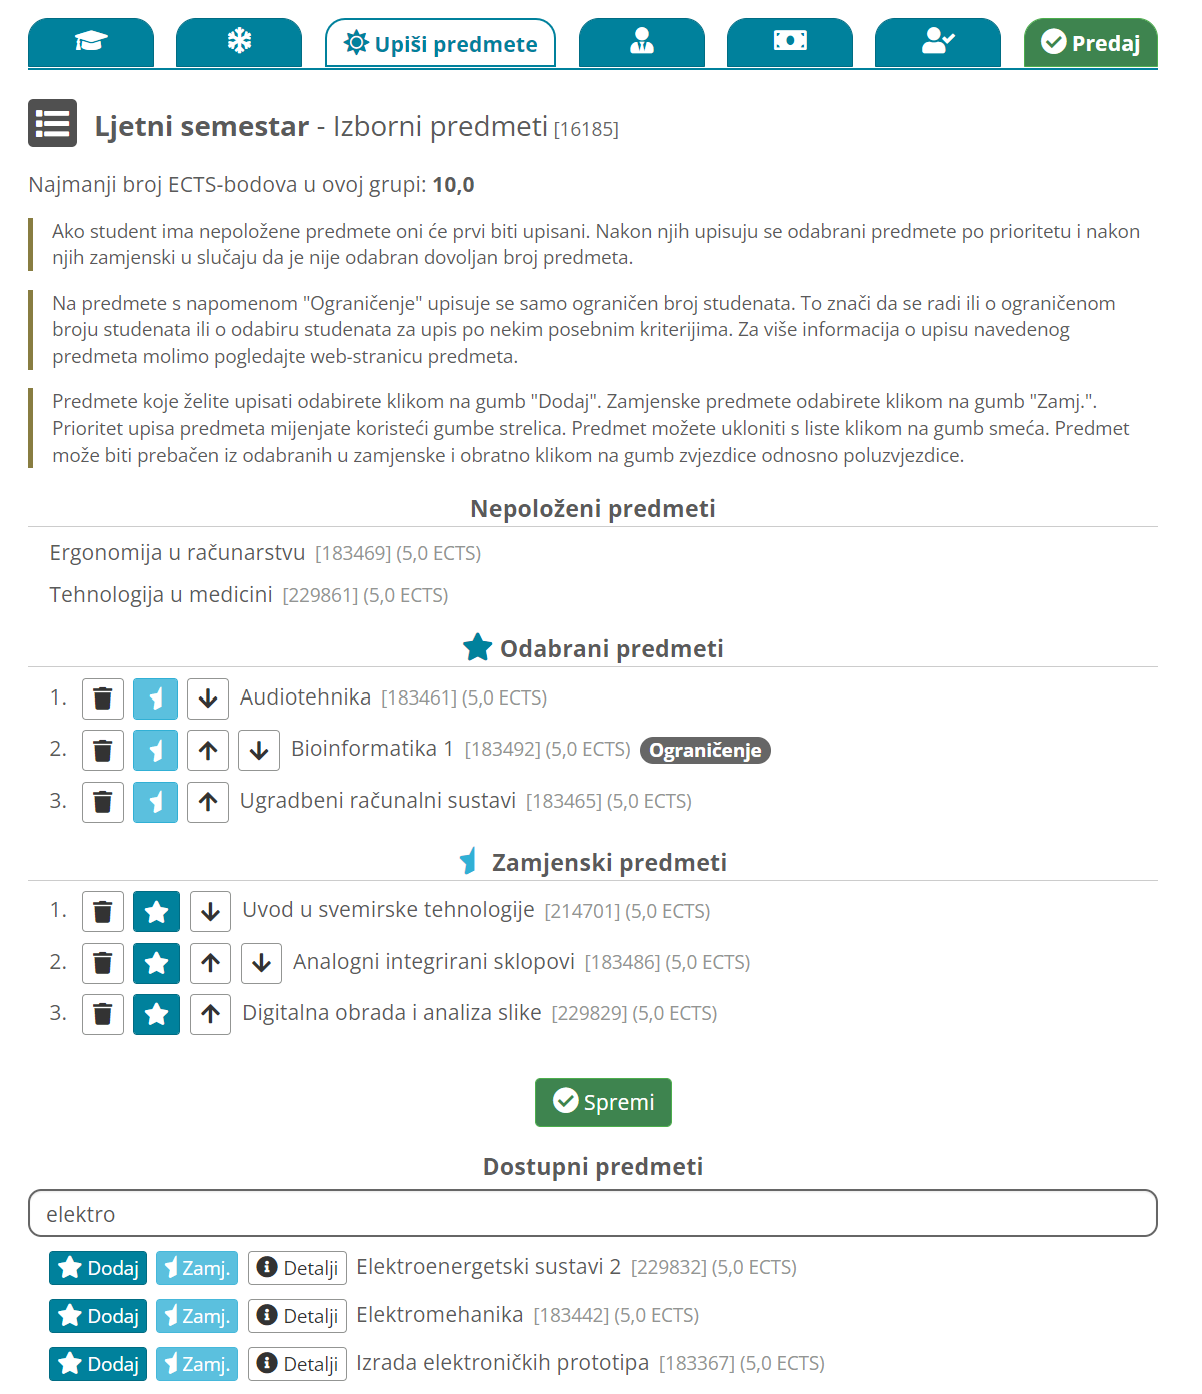
\includegraphics[scale=.6]{nova/selectcourses.png}}
      \centering
      \caption{Prikaz dijela stranice za odabir predmeta}
    \end{figure}
    
    \noindent\textbf{Mentor/ica}
    
    Na stranici imamo popis odabranih mentora i popis dostupnih mentora. Naslovi se nalaze na sredini stranice i popisi odmah ispod njih. Za odabrane mentore možemo mijenjati njihov redoslijed pomoću gumba sa strelicama ili ih ukloniti s popisa klikom na gumb s ikonicom kante za smeće. Kod promjene redoslijeda mentora prikazuju se animacije \textit{slideOutDown} i \textit{slideOutUp} iz biblioteke animate.css. Klikom na jednu od strelica mentori ne zamijene mjesta istog trenutka već je promjena napravljena brzom animacijom kako bi korisniku bilo jasnije da se neka promjena dogodila klikom na gumb. Klikom na gumb \textit{Odaberi} mentor je dodan na popis odabranih mentora. Dodavanje nije trenutačno nego ima animaciju \textit{fadeInLeft} iz biblioteke animate.css. Pri micanju mentora s popisa odabranih prikazuje se animacija \textit{fadeOutRight} iz biblioteke animate.css. Animacije su dodane iz istog razloga kao i pri mijenjaju redoslijeda. Korisniku animaciju privuče pozornost i bolje uočava promjenu izazvanu njegovim klikom gumba. Ispod popisa odabranih predmeta na sredini nalazi se gumb za spremanje korisnikovog odabira. Prije popisa dostupnih predmeta nalazi se search box. Na ovaj način korisnik ne mora tražiti željene mentore po dugačkom popisu, već može jednostavno pretraživati upisivanjem. Pretraživanje podržava upis imena, titule i kratice zavoda mentora. Za svakog dostupnog mentora klikom na gumb \textit{Info} prikazuje se prozor s više informacija o mentoru. Prozor se zatvara klikom na gumb \textit{Zatvori} koji se nalazi na mjestu gdje je gumb \textit{Info} bio prije otvaranja prozora.
    
    \begin{figure} [H]
      \fbox{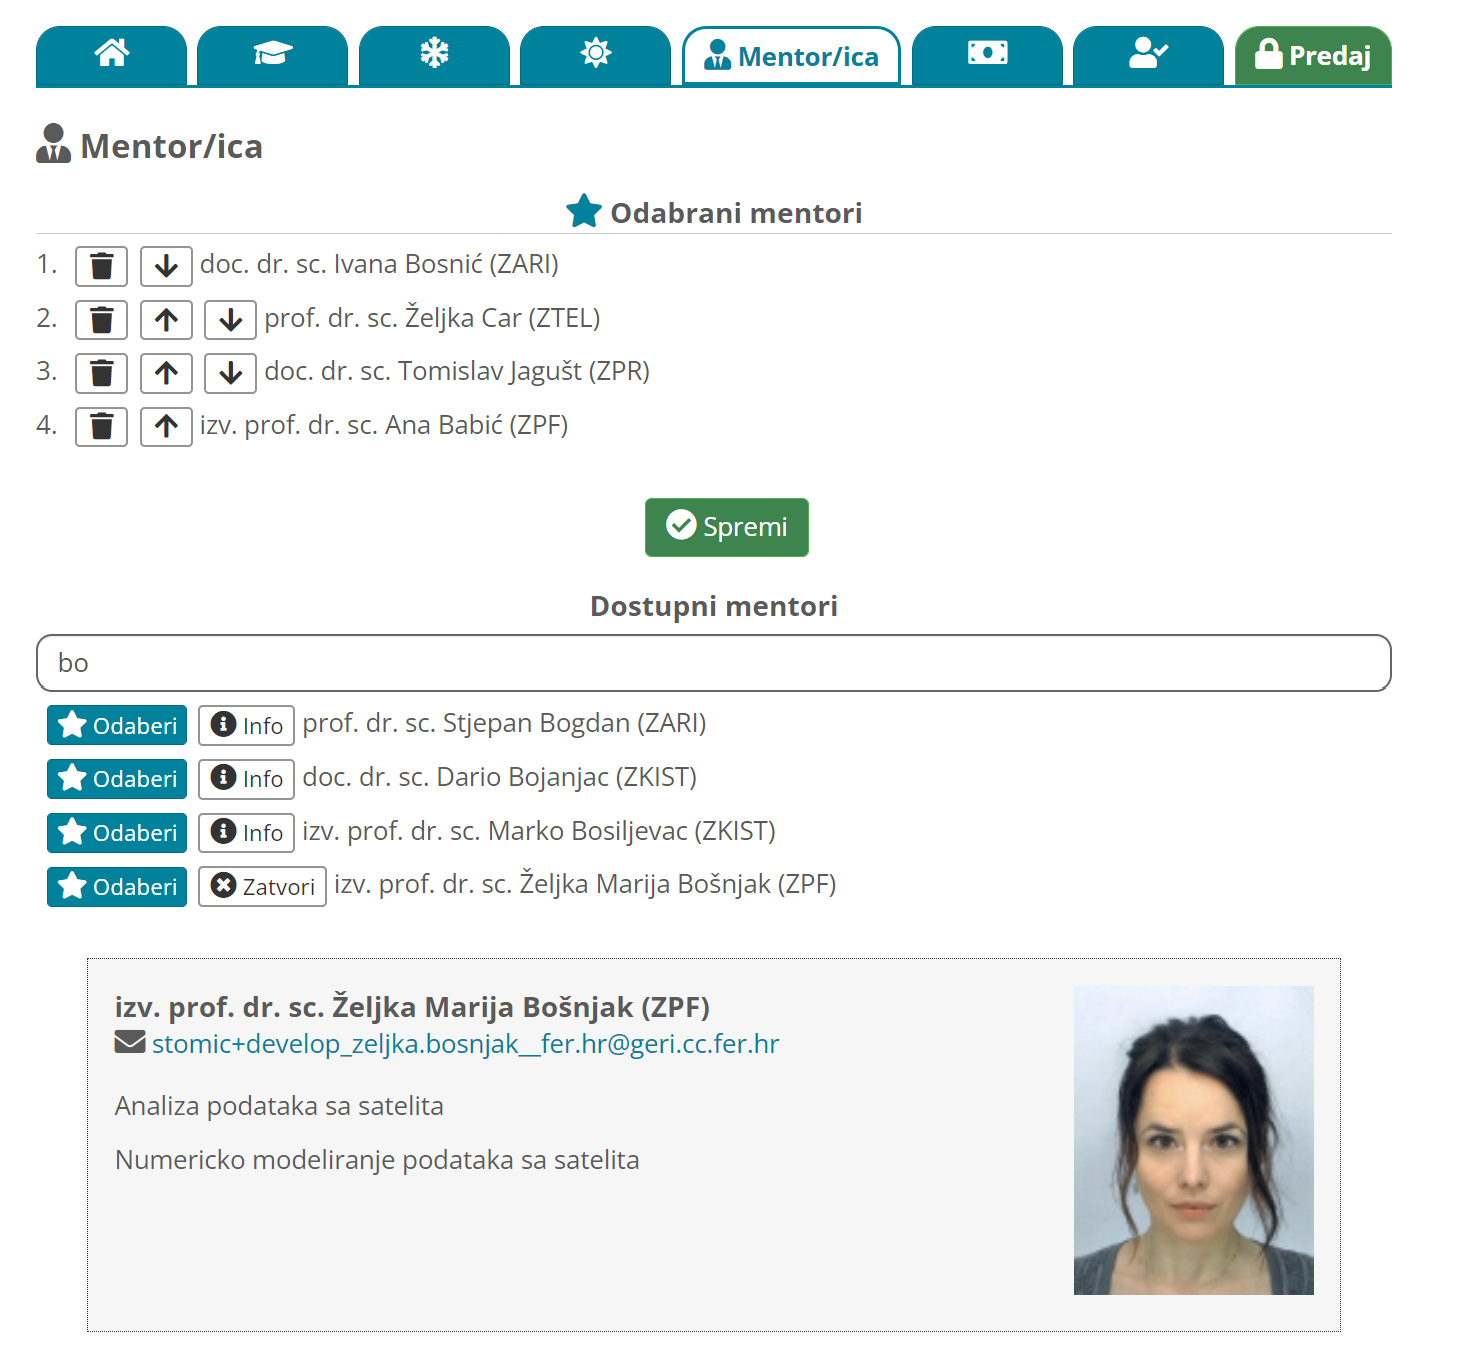
\includegraphics[scale=.45]{nova/mentor.png}}
      \centering
      \caption{Prikaz stranice odabira mentora}
    \end{figure}
    
    \noindent\textbf{Plaćanje}
    
    Na stranici plaćanja student može vidjeti svoje dugove i plaćanja te preuzeti račune na uređaj koji koriste. U tablici računa mogu se vidjeti iznos računa, datum plaćanja i napomena. Iznad tablice s popisom računa korisnik može vidjeti svoje ukupno trenutno dugovanje prikazano u kunama. Uklonjen je tekst iznad tablice i ostavljena samo informacija o ukupnom dûgu studenta s naglaskom na iznos u kunama koji je podebljan. U tablici je link \textit{Preuzmi} zamijenjen ikonicom preuzimanja kako bi se dodatno uklonio tekst i potreba za čitanjem. Svi studenti koji su sudjelovali u evaluaciji aplikacije, imali su primjedbe na prikaz u retcima tablice računa. Naime nije svaki redak nužno i račun. Jedan redak računa povezan je s jednim retkom potvrde o uplati i ta poveznica dvaju redaka nije nigdje prikazana. Nažalost, ovo nije rješivo s trenutnim načinom pohrane podataka u bazu. Kao alternativno rješenje na kraju stranice dodano je malo objašnjenje prikaza redaka u tablici. Na tablicu je dodan obrub kako se ne bi miješala s bijelom pozadinom.
    
    \begin{figure} [H]
      \fbox{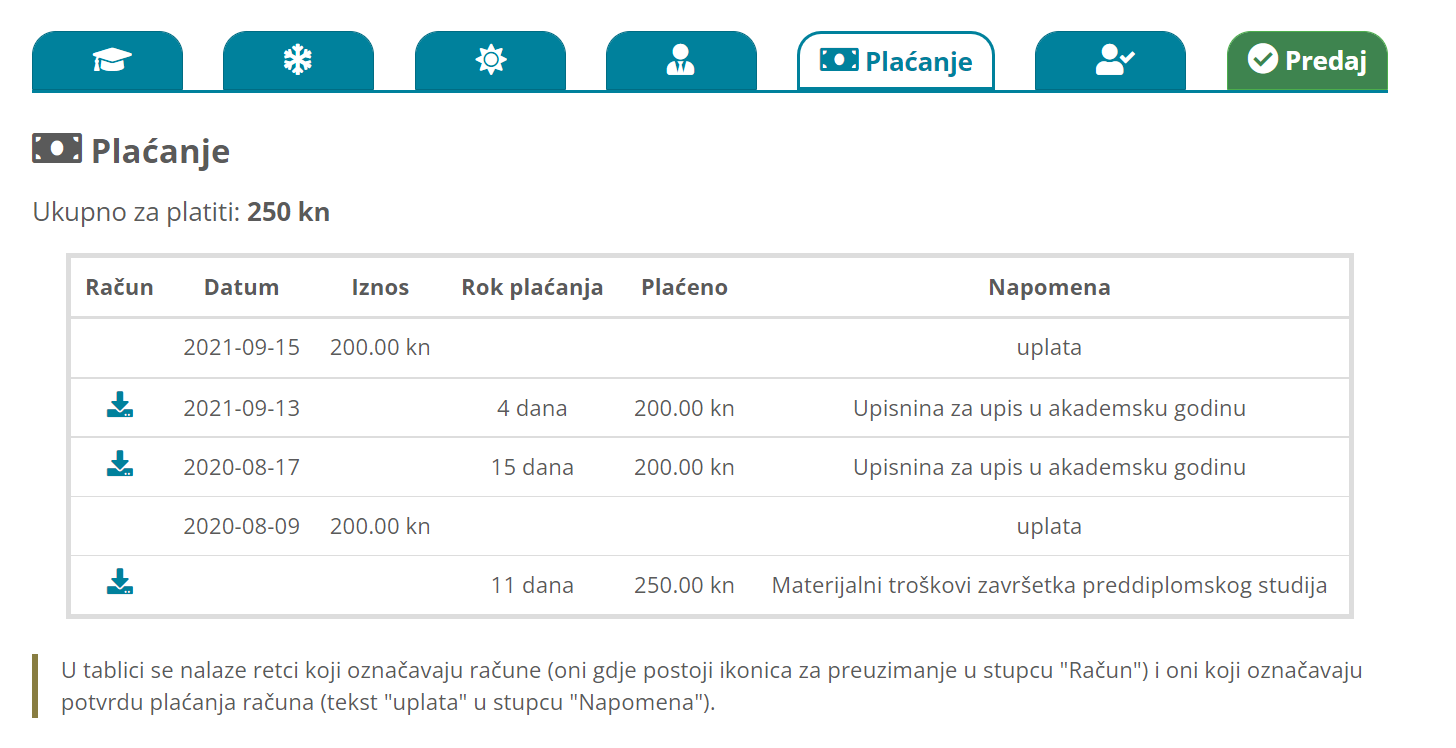
\includegraphics[scale=.5]{nova/placanje.png}}
      \centering
      \caption{Prikaz stranice računa}
    \end{figure}
    
    \noindent\textbf{Simulacija}
    
    Posljednji korak prije predaje prijave upisa godine je simulacija. U simulaciji student može vidjeti koji predmeti će mu biti upisani s obzirom na nepoložene predmete, položene predmete i odabrane predmete za upis. Uz svaki predmet postoji gumb za dopuštanje preklapanja s drugim predmetom. Izgled simulacije ostao je sličan onom na poboljšanom modulu uz razliku pozicioniranja naslova na sredini stranice umjesto lijevo. Objašnjenja vezana uz način rada simulacije prebačena su na dno stranice jer je većini korisnika intuitivno značenje elemenata na stranici i bitnije im je odmah vidjeti predmete koji se upisuju.
    
    \begin{figure} [H]
      \fbox{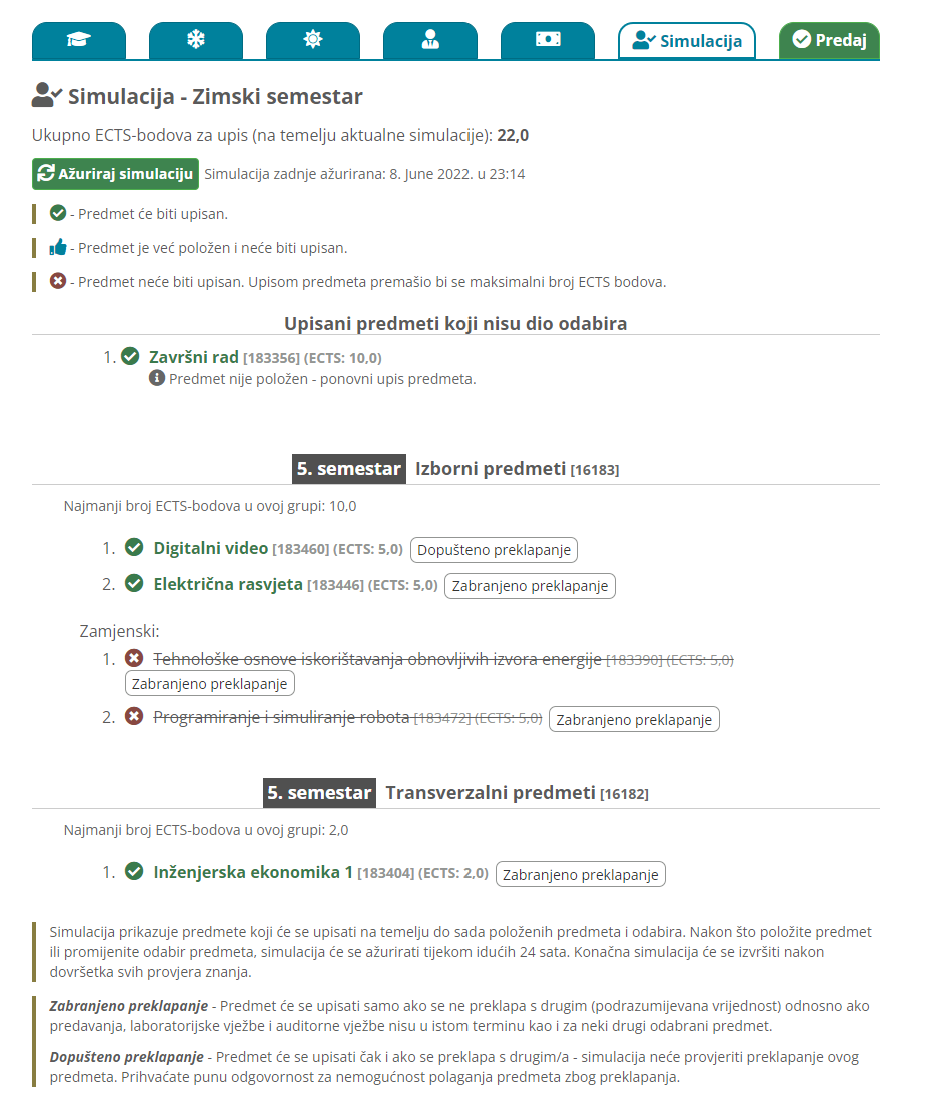
\includegraphics[scale=.6]{nova/simulacija.png}}
      \centering
      \caption{Prikaz stranice simulacije}
    \end{figure}
    
    Nigdje u aplikaciji nije korišten kurziv jer je s takvim tekstom ljudima s poteškoćama u čitanju otežano čitanje. Nijedno razlikovanje elemenata u aplikaciji ne ovisi isključivo o boji. Na mjestima gdje je poželjno stvoriti odvajanje elemenata korištene su i razlike u oblicima i dizajnu uz razliku u boji. Ovo je napravljeno imajući na umu korisnike s poteškoćama u prepoznavanju boja. Ako koristimo \textit{grayscale test} odnosno gledamo aplikaciju bez boje, koristeći samo crnu, bijelu i nijanse sive, korisnik bi i dalje trebao imati jednako iskustvo i s jednakom lakoćom uočiti razlike kao korisnik bez poteškoćama s bojama.
    
    \begin{figure} [H]
      \fbox{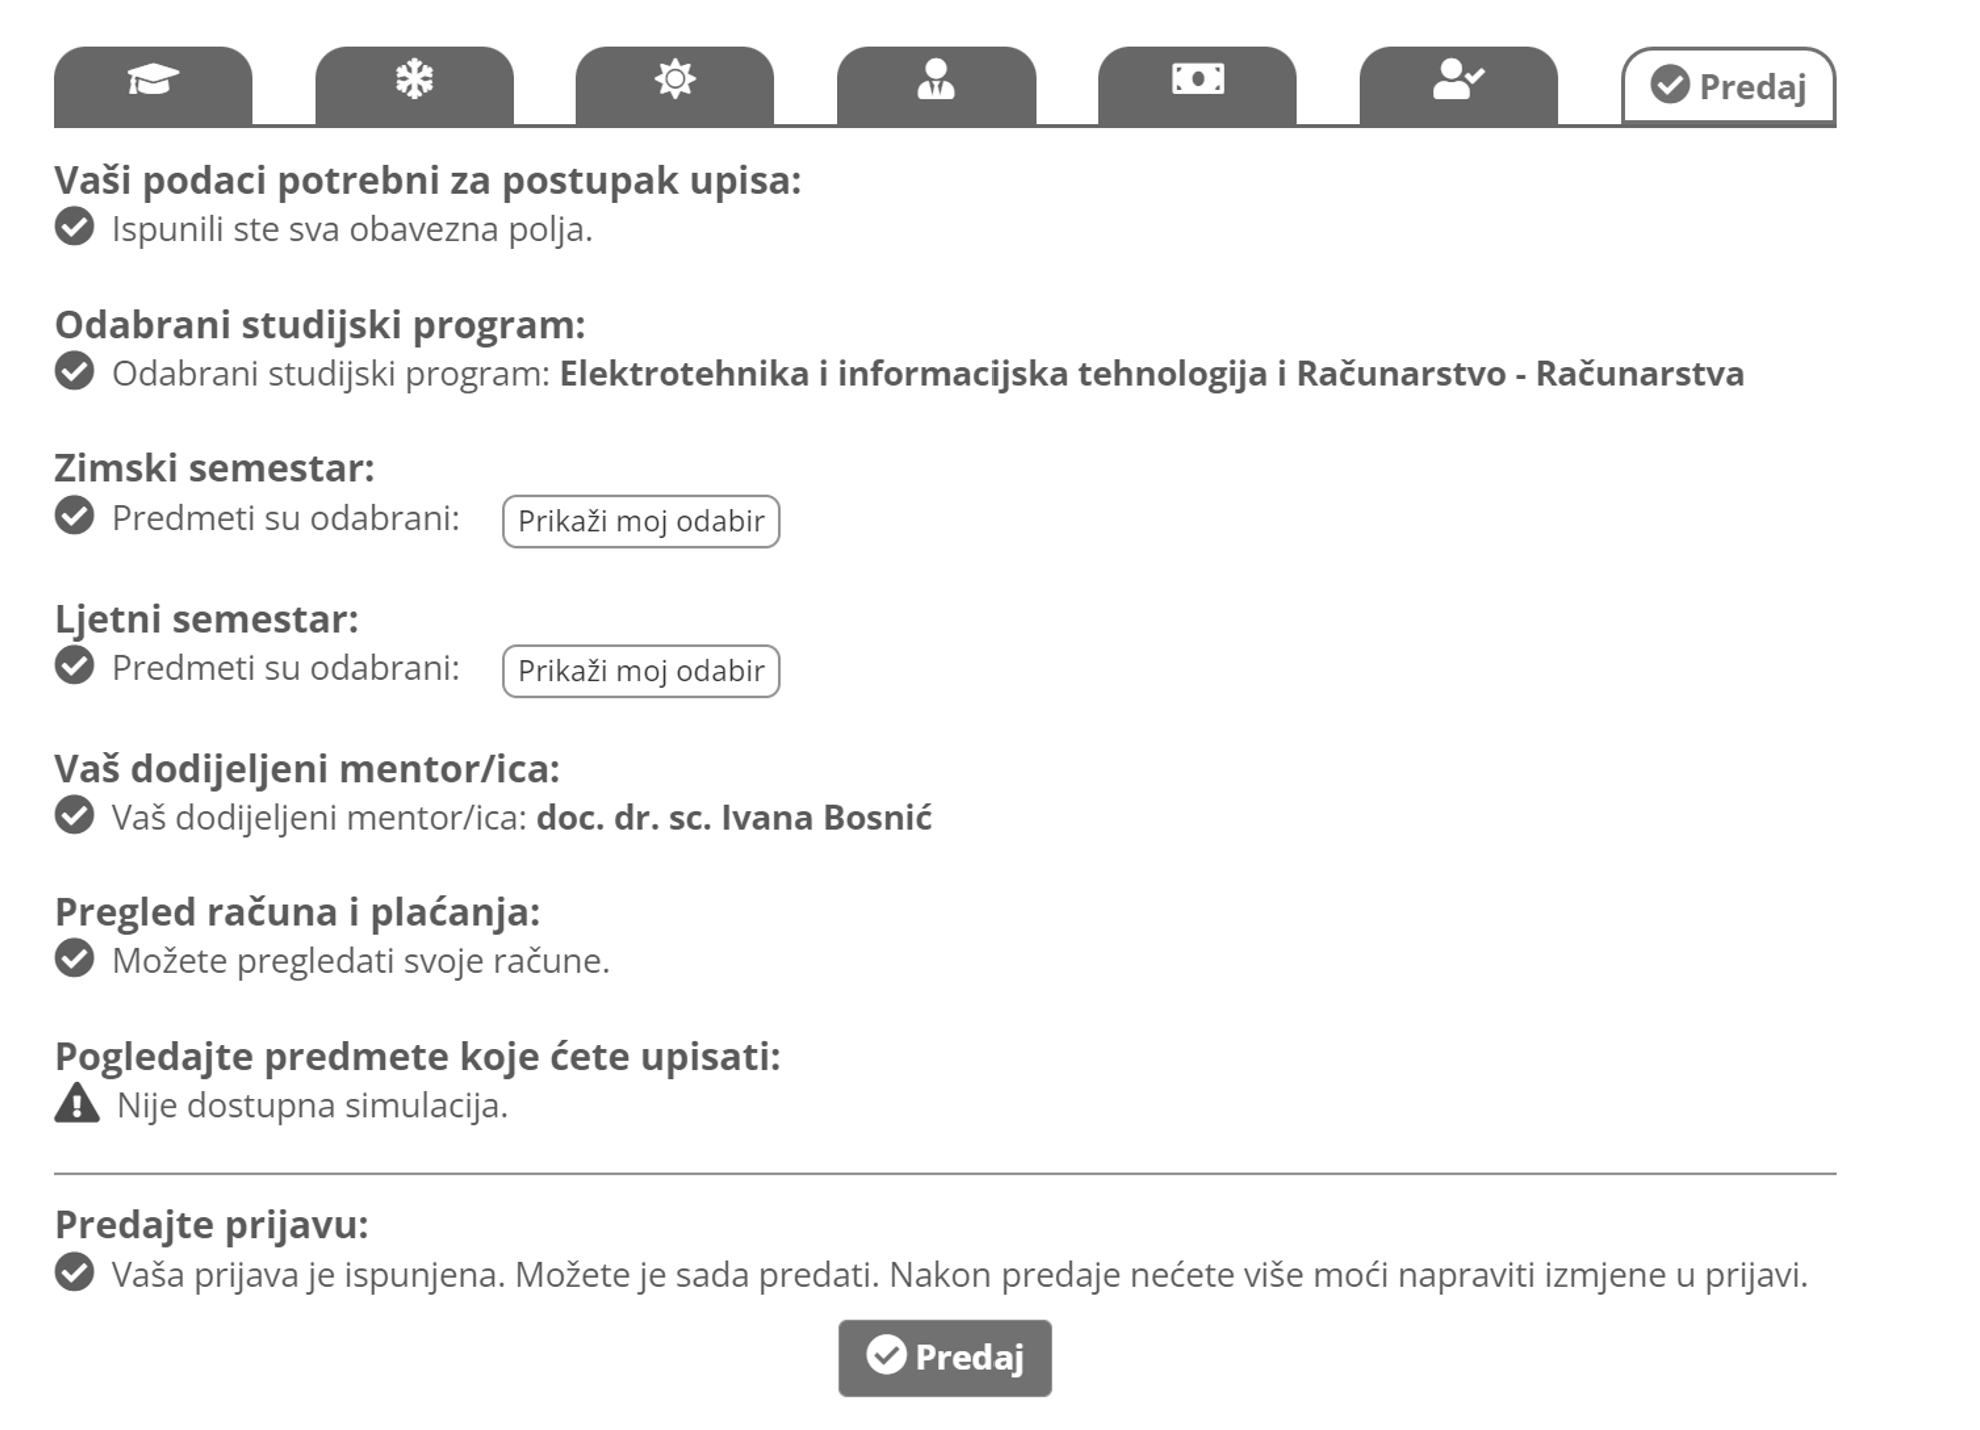
\includegraphics[scale=.5]{nova/gray.png}}
      \centering
      \caption{Monokromatski prikaz početne stranice}
      \label{fig:gray}
    \end{figure}
    
    Gledajući izgled početne stranice aplikacije kao osoba koja ne razlikuje boje možemo primijetiti kako plave kartice, zeleni gumb \textit{Spremi}, zelene kvačice i crveni trokut na slici \ref{fig:gray} izgledaju gotovo jednako. Ne oslanjajući se na boju kao primarnu oznaku različitih elemenata napravljeno je sučelje gdje korisničko iskustvo nije oduzeto osobama koje ne vide boju. One i dalje mogu prepoznati da je kod simulacije došlo do pogreške, da se nalazimo na kartici predaje te da kvačica označava ispravno popunjene korake.

    \section{Evaluacija novog dizajna}
    
    \textbf{Stranica prikaza semestara} i dalje je primila negativne kritike od strane studenata tijekom evaluacije novog dizajna aplikacije. Ovo je jedna od stranica koje narušavaju korisničko iskustvo zbog prikaza svih semestara.
    
    S obzirom da je dizajn stranica \textbf{odabira predmeta} poboljšane verzije aplikacije bio dobro prihvaćen od strane studenata tijekom evaluacije, dizajn nove aplikacije nije mnogo mijenjan. Glavna promjena bilo je polje za pretraživanje predmeta na stranici odabira predmeta. Ovakav dodatak funkcionalnosti bio je jedina tražena opcija od studenata tijekom evaluacije poboljšanog dizajna. Ovime je prosječna ocjena iskustva studenata pri korištenju stranica \textbf{odabira predmeta i prikaza semestara} aplikacije novog dizajna porasla i iznosi \textbf{4.4/5}.
    
    \begin{figure} [H]
      \fbox{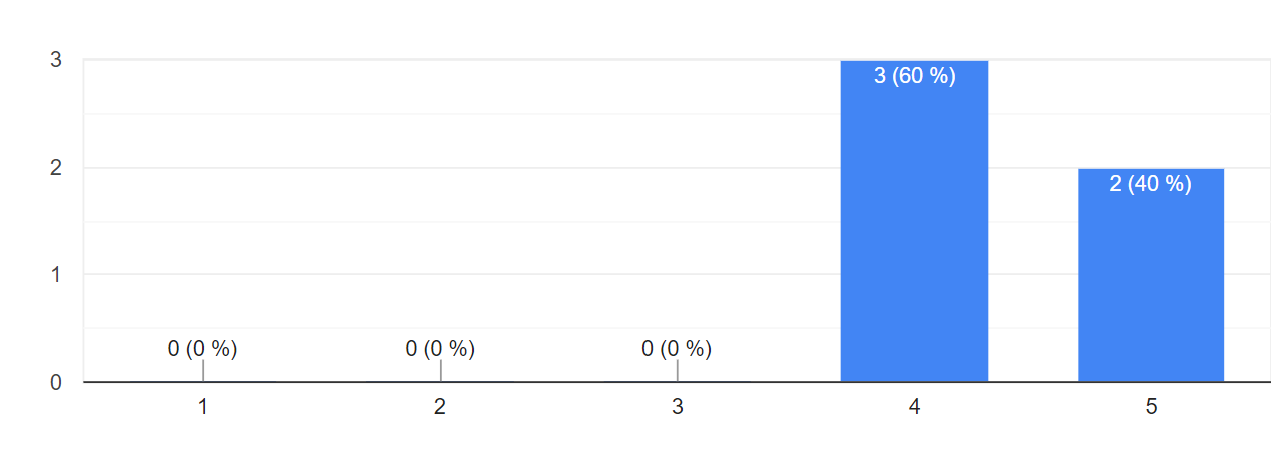
\includegraphics[scale=.5]{nova/courses_ocjena.png}}
      \centering
      \caption{Ocjene korisničkog iskustva prikaza semestara i biranja predmeta na aplikaciji novog dizajna}
    \end{figure}
    
    Promjene u izgledu stranice studijskog programa bile su pohvaljene tijekom evaluacije.
    
    Stranica plaćanja je tijekom ove evaluacije bila prihvaćena više nego tijekom prijašnjih procjena. Uklonjen je sav nepotreban tekst i ostavljen je samo podatak o ukupnom dûgu i računima što je jedino što studente na toj stranici i zanima. Nakon dodavanja obruba na tablicu, bilo je manje kritika na njezinu neobičnu strukturu i izgled. Na ovo je utjecaj imala i poruka na dnu stranice koja kratko objašnjava značenje redaka u tablici. Uz stranicu prikaza semestara, stranica plaćanja najviše narušava iskustvo studenata pri upisu zbog načina implementacije računa u bazu podataka. Prosječna ocjena iskustva studenata pri korištenju \textbf{stranice plaćanja} aplikacije novog dizajna je \textbf{3.8/5}.
    
    \begin{figure} [H]
      \fbox{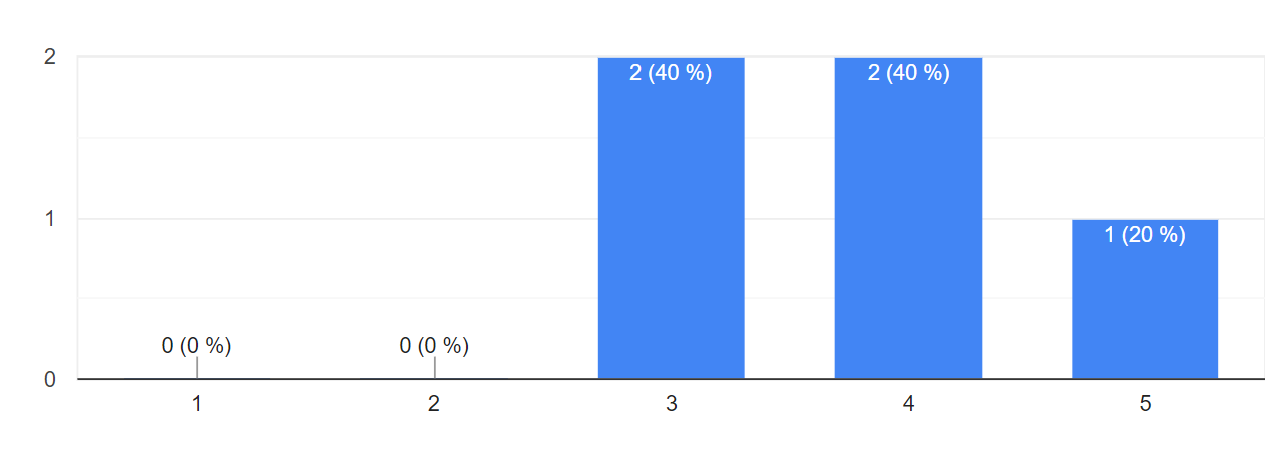
\includegraphics[scale=.5]{nova/placanje_ocjena.png}}
      \centering
      \caption{Ocjene korisničkog iskustva stranice plaćanja na aplikaciji novog dizajna}
    \end{figure}
    
    Stranica promjene ECTS-bodova ostala je jednaka, a stranica simulacije skoro identična onoj u poboljšanom dizajnu. Studenti nisu istaknuli nedostatke ovih stranica u prošloj evaluaciji, kao ni u ovoj.
    
    Nakon evaluacije cijele aplikacije, studenti su dali svoje završne ocjene temeljene na svojem iskustvu upisa. Prosječna ocjena iskustva studenata pri korištenju aplikacije novog dizajna je \textbf{4.2/5}.
    
    \begin{figure} [H]
      \fbox{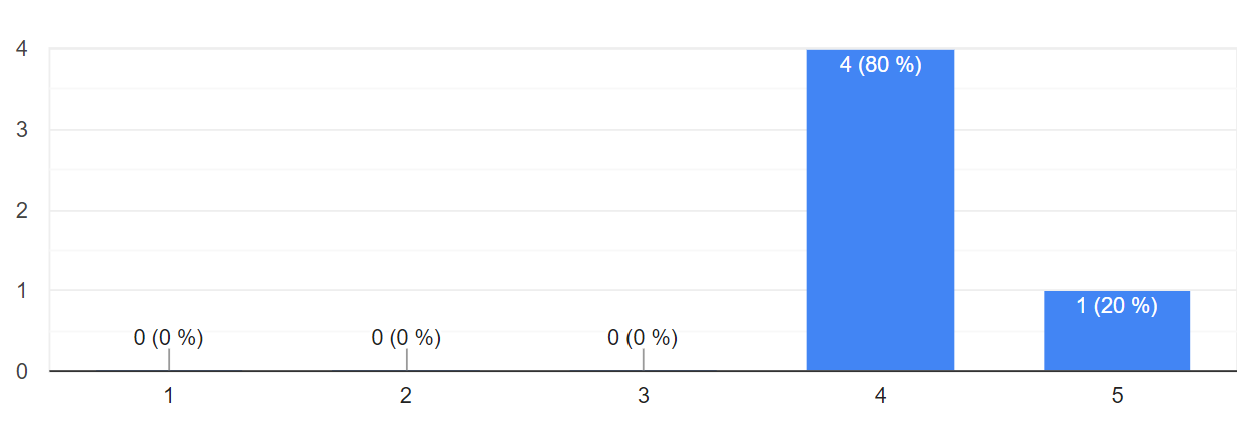
\includegraphics[scale=.5]{nova/overall.png}}
      \centering
      \caption{Ocjene korisničkog iskustva aplikacije novog dizajna}
    \end{figure}


\chapter{Izrada poboljšanog i novog modula}
    %Tehnoloski opis, struktura modula, što se mijenja, kako se mijenja, vazne funkcije
    %\section{Korištene biblioteke}
    %bla
    %\section{Izrada poboljšanog i novog dizajna}
    %\section{Struktura modula}
    %struktura modula
    Aplikacija za upis akademske godine rađena je koristeći verziju 2 programskog okvira (\textit{Framework}) \textbf{Vue.js}\footnote{https://vuejs.org/}. To je radni okvir jezika JavaScript i koristi se za izradu korisničkih sučelja na webu.
    
    Način rada poboljšanog modula i modula novog dizajna identičan je zbog interne implementacije strukture i povezanosti stranica. Osnovna datoteka za rad modula je \textit{App.vue}. Ona se nalazi u mapi \textit{src} zajedno s mapama \textit{common} i \textit{views}.
    
    U mapi \textit{common} nalaze se datoteke u kojima su definirane rute, API funkcije, datoteka koja omogućuje dvojezičnost modula te mapa \textit{locales} u kojoj su \textit{hr.json} i \textit{en.json} datoteke s hrvatskim i engleskim prijevodima svog teksta koji se na modulu nalazi.
    
    Modul se sastoji od nekoliko stranica po kojima se korisnik kreće koristeći vizualne navigacijske elemente. Kôd svake pojedinačne stranice nalazi se u mapi \textit{views}. Jedna stranica je jedna .vue datoteka. Svaka od njih ima korijensku HTML oznaku (\textit{root HTML tag}) \textit{<template>} u kojoj se nalazi sam HTML-kôd te stranice. Osim oznake \textit{<template>}, stranica ima i svoj JavaScript kôd koji se nalazi u oznaci \textit{<script>}. Posljednja oznaka u datotekama je \textit{<style scoped>} u kojoj je zapisan sav CSS specifičan za tu stranicu. U slučaju da se CSS odnosi na sve stranice, on se nalazi u kasnije spomenutoj datoteci \textit{style.css}.
    
    U istoj razini kao \textit{src} mapa nalaze se i mape \textit{components} i mapa \textit{public}. U mapi \textit{components} nalaze se posebno izrađene \textbf{komponente} korištene na određenim stranicama. Komponente omogućuju podjelu korisničkog sučelja na nezavisne dijelove koji se mogu ponovno koristiti.
    
    U mapi \textit{public}, koja je u razini mape \textit{src}, nalaze se sve korištene \textbf{CSS} datoteke. To su \textit{animate.css}, \textit{tooltips.css} i \textit{style.css}. U ovoj mapi također se nalazi datoteka \textit{index.html} u koju je ubačena glavna datoteka \textit{App.vue} iz koje je modul izrađen.
    
    U poboljšanom i novom dizajnu za animaciju pri promjeni stranice korištena je \textit{Vue.js} komponenta \textit{<Transition>}. Komponenta treba zamatati element koji je potrebno animirati. Kako je u modulima ona korištena za animaciju promjene stranica, dodana je u \textit{App.vue} datoteku preko elementa \textit{<router-view>}. Dodano joj je ime za kasnije stiliziranje:
    \begin{verbatim}
    <Transition name="router-anim" >
        <router-view>
        </router-view>
    </Transition>
    \end{verbatim}
    
    Kod modula poboljšanog dizajna, stranica se pri izlazu translatira ulijevo, a pri ulazu udesno zbog vertikalnog položaja gumba na početnoj stranici. Kod modula novog dizajna, ovo je promijenjeno da se stranica translatira gore pa dolje zbog horizontalnog položaja gumba na početnoj stranici modula.
        
    Na novom dizajnu dodana je animacija koja se aktivira akcijom \textit{hover} nad karticama. Kada korisnik pozicionira miš na jednu od kartica, ona će se animirano proširiti i prikazati naziv kartice. Na ovaj način, ako korisnik ne zna što očekivati na kojoj kartici, to može saznati bez da je prisiljen odlaziti na stranicu te kartice.
    
    Svakoj od kartica dodan je odgovarajući ID na element \textit{<a>} i klase za tekst. Ovo je primjer za karticu studijskog programa:
    \begin{verbatim}
    <a
        id="studijski-tab"
        class="btn btn-primary tab"
        @click="navigate"
        :href="href">
        <div class="tab-text-combo">
            <i class="fas fa-graduation-cap"></i>
            <span class="tab-text"> 
                {{$t("profile")}}
            </span>
        </div>
    </a>
    \end{verbatim}
    
    Ove klase i ID uređeni su u \textit{style.css} datoteci:
    \begin{verbatim}
    #upisi-predmete-tab {
        position: relative;
        transition: min-width 0.3s ease-in-out;
    }
    #upisi-predmete-tab:hover {
        min-width: 17.5rem;
    }

    #upisi-predmete-tab:hover>.tab-text-combo {
        left: 10%;
    }

    #upisi-predmete-tab:hover>.tab-text-combo>.tab-text {
        opacity:1;
    }
    \end{verbatim}
    \section{Rad s bibliotekom animate.css}
    %sto se mijenja, kako se mijenja, funkcije
    Za dodavanje pokretnog dizajna u module pretežno je korištena biblioteka \textit{animate.css}\footnote{https://animate.style/}. Za korištenje biblioteke potrebno ju je instalirati na računalo. Ovo je moguće obaviti pokretanjem jedne od sljedećih naredbi iz komandne linije:
    \begin{verbatim} npm install animate.css --save \end{verbatim}
    \begin{verbatim} yarn add animate.css \end{verbatim}
    Nakon instalacije potrebno je uvesti (\textit{import}) biblioteku u željenu datoteku što je u slučaju naših modula izgledalo ovako: \begin{verbatim} import '../../public/animate.css';\end{verbatim} 
    
    Biblioteka sadrži mnogo animacija koje su na njihovoj web-stranici podijeljene po ulogama. U poboljšanom i novom dizajnu korištene su \textit{Fading entrances}, \textit{Fading exits} i \textit{Sliding exits}. Ovo su suptilne animacije korištene za isticanje posljedica korisnikovih akcija. Za dodavanje animacije na element potrebno je kao jednu od klasa elementa dodati klasu \textit{animate\_\_animated}. Sada je na taj element moguće dodati željenu animaciju.
    
    U datotekama \textit{SelectCourses.vue} i \textit{SelectMentor.vue} na strelice za promjenu redoslijeda predmeta i mentora na popisima dodane su animacije \textit{slideOutUp} i \textit{slideOutDown}. Ovo je implementirano na način da se animacije dodaju na elemente kada je kliknut gumb strelice i pozvana funkcija za promjenu. Za prikaz implementacije bit će korištena stranica odabira mentora.
    
    Elementi \textit{<div>}, čija su djeca elementi gumba te podaci mentora, generiraju se \textit{for-in} petljom. Njemu je dodana klasa \textit{animate\_\_animated} i kao ID je stavljen element \textit{for-in} petlje:
    \begin{verbatim}
    <div class="animate__animated" :id=item>
    \end{verbatim}
    Pri kliku jedne od strelica za promjenu redoslijeda poziva se funkcija \textit{selectedMove} koja kao parametre prima \textit{key} i brojeve 1 ili -1 koja je vezana na gumb sa strelicom:
    \begin{verbatim} @click="selectedMove(key, 1)" \end{verbatim}
    Parametar \textit{key} označava redni broj određenog mentora u listi odabranih mentora. Broj 1 označava kako korisnik želi podići prioritet mentora, a -1 kako ga želi spustiti. Kada se mentora želi prebaciti na više mjesto u listi, tada se na označenog mentora dodaje animacija \textit{slideOutUp}, a na onog s kojim će se prioritet zamijeniti dodaje se \textit{slideOutDown}. Animacije se dodaju tako da se na spomenuti \textit{<div>} element dodaju klase animacija:
    \begin{verbatim}
    document.getElementById(this.mentors[item])
     .classList.add('animate__slideOutUp')
     document.getElementById(this.mentors[broj])
     .classList.add('animate__slideOutDown')
    \end{verbatim}
    gdje je \textit{item} jednak broju mentora u listi mentora \textit{mentors}.
    
    U datoteci \textit{Index.vue} dodana je animacija \textit{fadeInLeft} na posljednji korak prijave. Animacija je aktivira pri učitavanju tog dijela stranice stoga je klasa animacije dodana direktno u \textit{<div>} element s gumbom predaje i tekstom vezanim za taj korak:
    \begin{verbatim} <div class="animate__animated animate__fadeInLeft"> \end{verbatim}
    Mjesto na kojem je još korištena ova animacija je u \textit{SelectCourses.vue} odnosno na stranici odabira predmeta. Ondje se ova animacija koristi pri dodavanju predmeta iz liste dostupnih u listu odabranih ili zamjenskih i za prebacivanje iz lista željenih predmeta međusobno. Pri uklanjanju predmeta s liste koristi se animacija \textit{fadeOutRight}. Klasa \textit{animate\_\_animated} dodana je na \textit{<div>} element koji sadrži naziv predmeta i gumbe za upravljanje tim predmetom. Elementu je dodijeljen i ID koji je specifičan za svaki predmet:
    \begin{verbatim}
    <div class="animate__animated" :id=item.course_id>
    \end{verbatim}
    Pri kliku na gumb za uklanjanje predmeta poziva se funkcija \textit{removeSelected} koja prima parametar \textit{item} što je objekt predmeta u listi predmeta:
    \begin{verbatim}
    @click="removeSelected(item)"
    \end{verbatim}
    U kôdu, na početku funkcije napisana je linija za dodavanje klase: \begin{verbatim}
    document.getElementById(item.course_id)
     .classList.add('animate__fadeOutRight')
    \end{verbatim}
    
    Animacije \textit{fadeInDown} i \textit{fadeOutUp} korištene su na početnom ekranu odnosno implementirane u \textit{Index.vue} datoteku. Prikazuju se pri kliku na gumb \textit{Prikaži moj odabir} za svaki od semestara. Implementirane su na isti način kao i ostale spomenute animacije.
    
    \textit{Animate.css} mala je biblioteka koja sadrži korisne animacije. Korištenje biblioteke veoma je jednostavno i sadržane animacije mogu činiti odličan dodatak web-stranicama i aplikacijama. Dodavanje ovih jednostavnih animacija značajno je poboljšalo iskustvo korisnika pri korištenju aplikacije za upis u godinu.
    
    \section{Rad s bibliotekom Effeckt.css}
    Druga biblioteka pokretnog dizajna korištena u izradi novih modula je \textit{Effeckt.css}\footnote{https://h5bp.org/Effeckt.css/}. Iz ove biblioteke korištena je opcija info-oblačića u poboljšanom i u novom dizajnu. Implementirani su info-oblačići na stranici odabira predmeta korištenjem ove biblioteke. Akcijom \textit{hover} nad oznakama \textit{Ograničenje}, \textit{Ne održava se} i \textit{Nije moguće upisati} pojavi se oblačić s kratkim objašnjenjem iznad oznake. Ovo je implementirano na način da su ovi \textit{<span>} elementi omotani elementom \textit{<a>} koji sadrži potreban kôd za rad info-oblačića:
    \begin{verbatim}
    <a href="#0"
     :data-effeckt-tooltip-text='$t("course_limit_desc")'
     class="effeckt-tooltip" data-effeckt-type="bubble"
     data-effeckt-position="top">
    \end{verbatim}

    U usporedbi s \textit{animate.css} ova biblioteka je opsežnija. Sadrži animacije za modale, gumbe, liste i ostalo. Iako ova biblioteka ima više mogućnosti nego \textit{animate.css}, mnoge su animacije napravljene preupečatljivo. Većina njih bi svojom implementacijom pogoršale korisničko iskustvo. Samo neke od postojećih animacija su dovoljno suptilne da prenesu povratnu informaciju korisniku bez da u potpunosti odvuku njegovu pozornost i nepotrebno ga zaokupiraju.
    
\chapter{Usporedba dizajna}
    Prije izrade novog dizajna obavljeno je kratko istraživanje na postojećem. Ono je pokazalo kako su određene stranice problematičnog izgleda i narušavaju iskustvo studenata koji upisuju novu akademsku godinu. To su bile \textbf{stranica plaćanja računa te stranice prikaza semestara i biranja predmeta}. Izgled i iskustvo studenata pri korištenju tih stranica ocjenjivano je u daljnjim evaluacijama za poboljšani i novi dizajn kako se bi se lakše pratila efikasnost promjena u izgledu. Tablica koja slijedi prikazuje spomenute ocjene.
    
    \begin{table}[H]
    \begin{center}
    \caption{\label{tab:table-name}Usporedba prosječnih ocjena dobivenih evaluacijama}
    \begin{tabular}{ |c|c|c|c| }
    \hline
    & \textbf{stari} & \textbf{poboljšani} & \textbf{novi} \\
    \hline
    \textbf{prikaz semestara i biranje predmeta} & 3.8 & 4.2 & 4.4\\
    \hline
    \textbf{plaćanje} & 1.8 & 2 & 3.8\\
    \hline
    \textbf{ukupno} & 3.2 & 4 & 4.2\\ 
    \hline
    \end{tabular}
    \end{center}
    \end{table}
    
    \noindent\textbf{Prikaz semestara i odabir predmeta}
    
    Naslov \textit{Predmeti} koji se nalazi na početku postojećeg modula jednak je kao i naslov kod odabira predmeta. U poboljšanom i novom dizajnu ovo je promijenjeno u naslov odgovarajućeg imena koji bolje opisuje funkcionalnost stranice.
    
    Na oba nova dizajna dodana je poruka na vrhu kako bi studenti znali da sami trebaju obratiti pozornost na to u kojem semestru trebaju upisati predmete.
    
    Postojeća hijerarhija između grupa predmeta, teksta o minimalnom broju ECTS-bodova za upis, popisu odabranih predmeta i gumbu za odabir predmeta promijenjena je na poboljšanom dizajnu na način da postoji samo jedno uvlačenje elemenata udesno. Ovime je popravljen odnos elemenata međusobno. Na poboljšanom i novom dizajnu povećani su razmaci između grupa predmeta i dodana je slaba pozadinska boja da bolje odjeljuje semestre. Zbog načina pohrane podataka u bazu koju aplikacija koristi, nije moguće implementirati pregled grupa semestara harmonikom što bi učinilo dizajn jasnim za korisnika. Istaknutim promjenama stranica izgleda preglednije. Također, u oba rađena dizajna podebljani su nazivi odabranih predmeta kako bi bili uočljiviji. Kod poboljšanog dizajna pozadina gumba \textit{Odabir predmeta} promijenjena je u neutralnu plavu boju, a kod novog dizajna ima bijelu pozadinu s plavim obrubom i plavim tekstom kako gumb ne bi bio zamijenjen s karticama na vrhu stranice. Naslovi grupa po semestrima i ostali elementi su centrirani na novom dizajnu.
    
    Navedenim promjenama važnost stranice prebačena je na odabrane predmete.
    
    \begin{figure} [H]
      \fbox{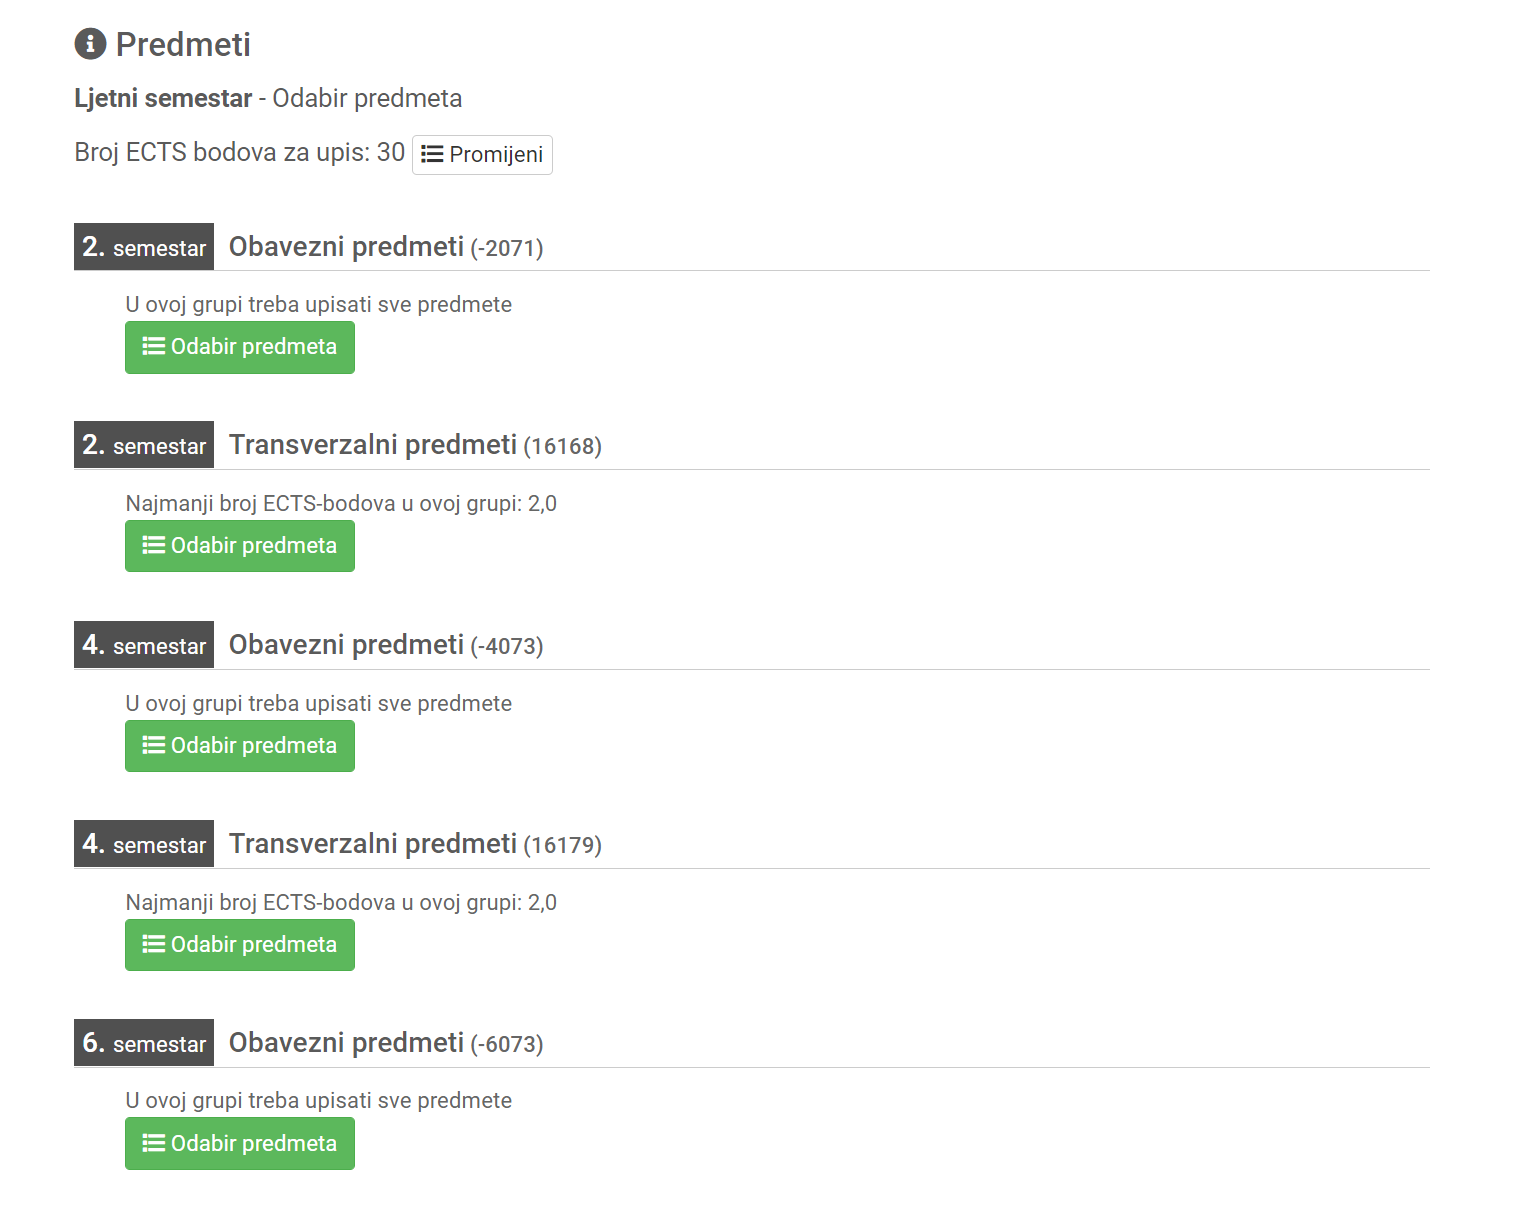
\includegraphics[scale=.5]{stara/courses_1.png}}
      \fbox{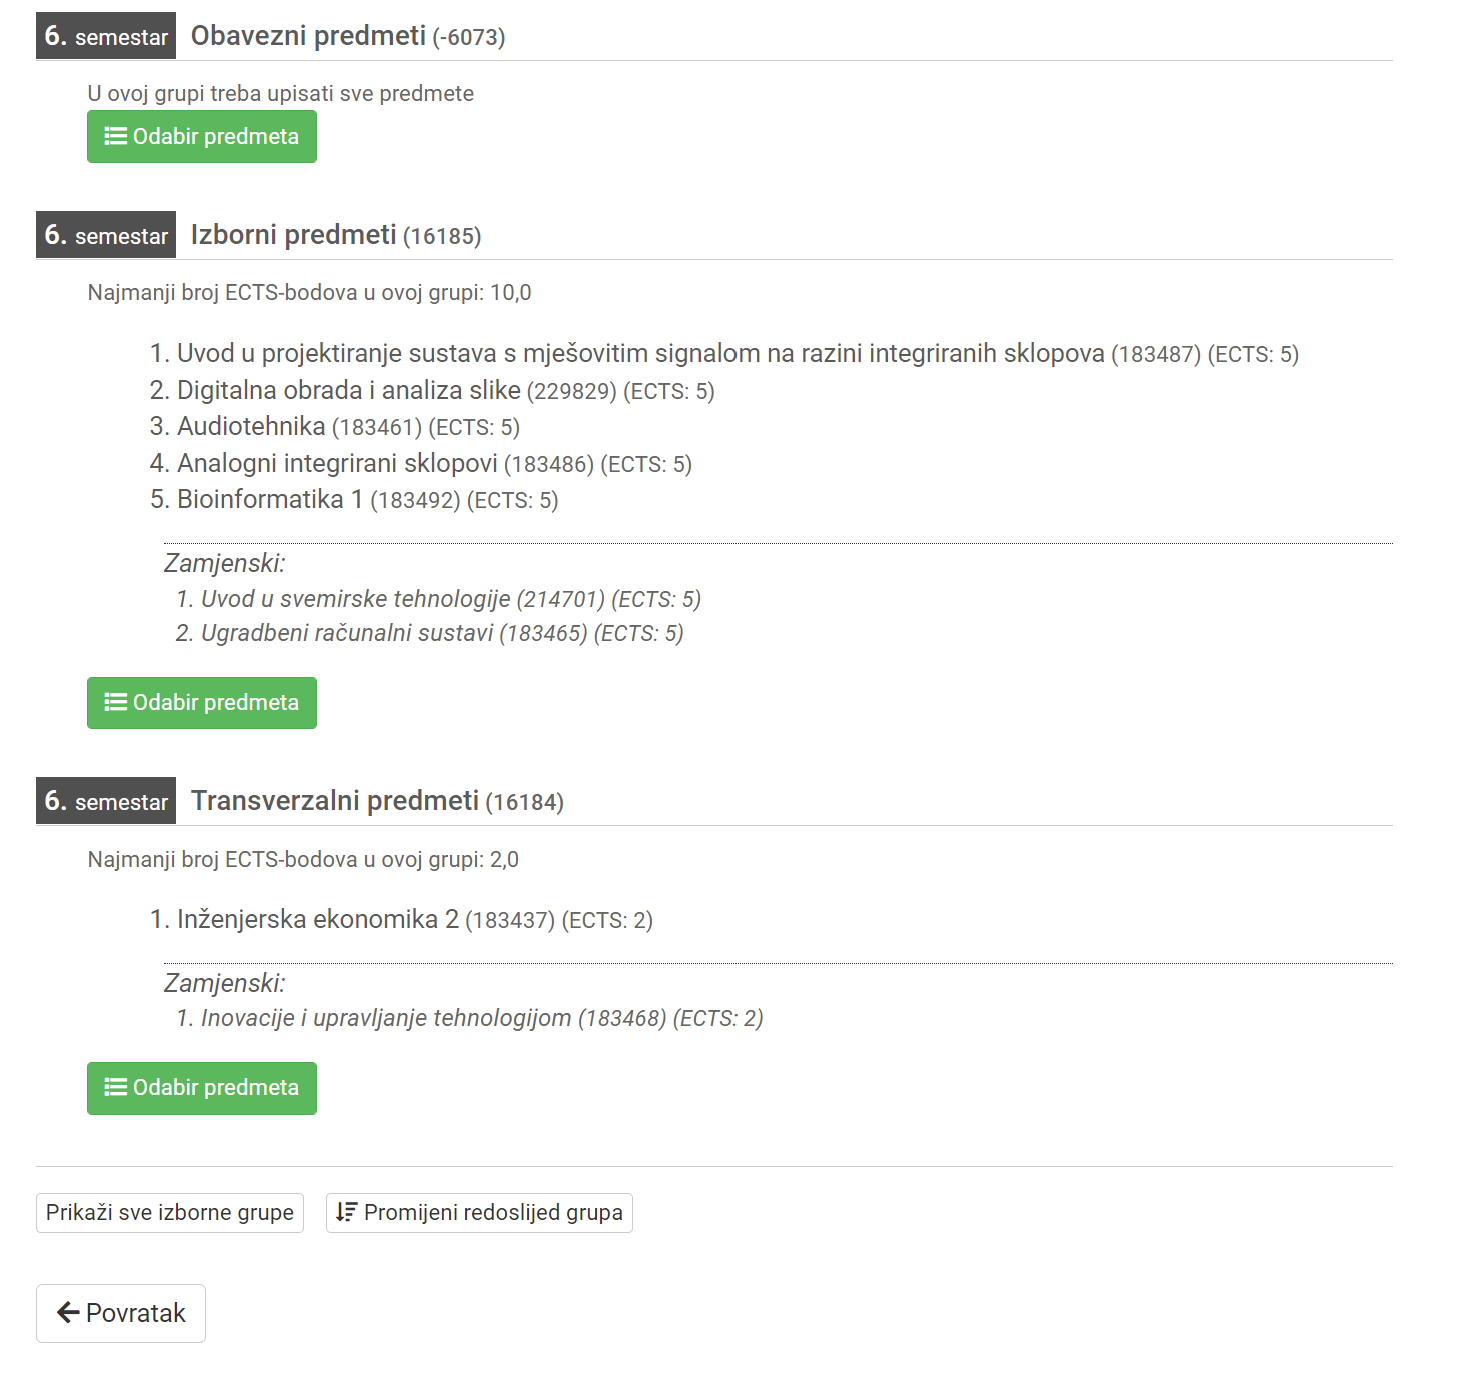
\includegraphics[scale=.5]{stara/courses_2.png}}
      \centering
      \caption{Prikaz odabira semestara aplikacije starog dizajna}
    \end{figure}
    
    \begin{figure} [H]
      \fbox{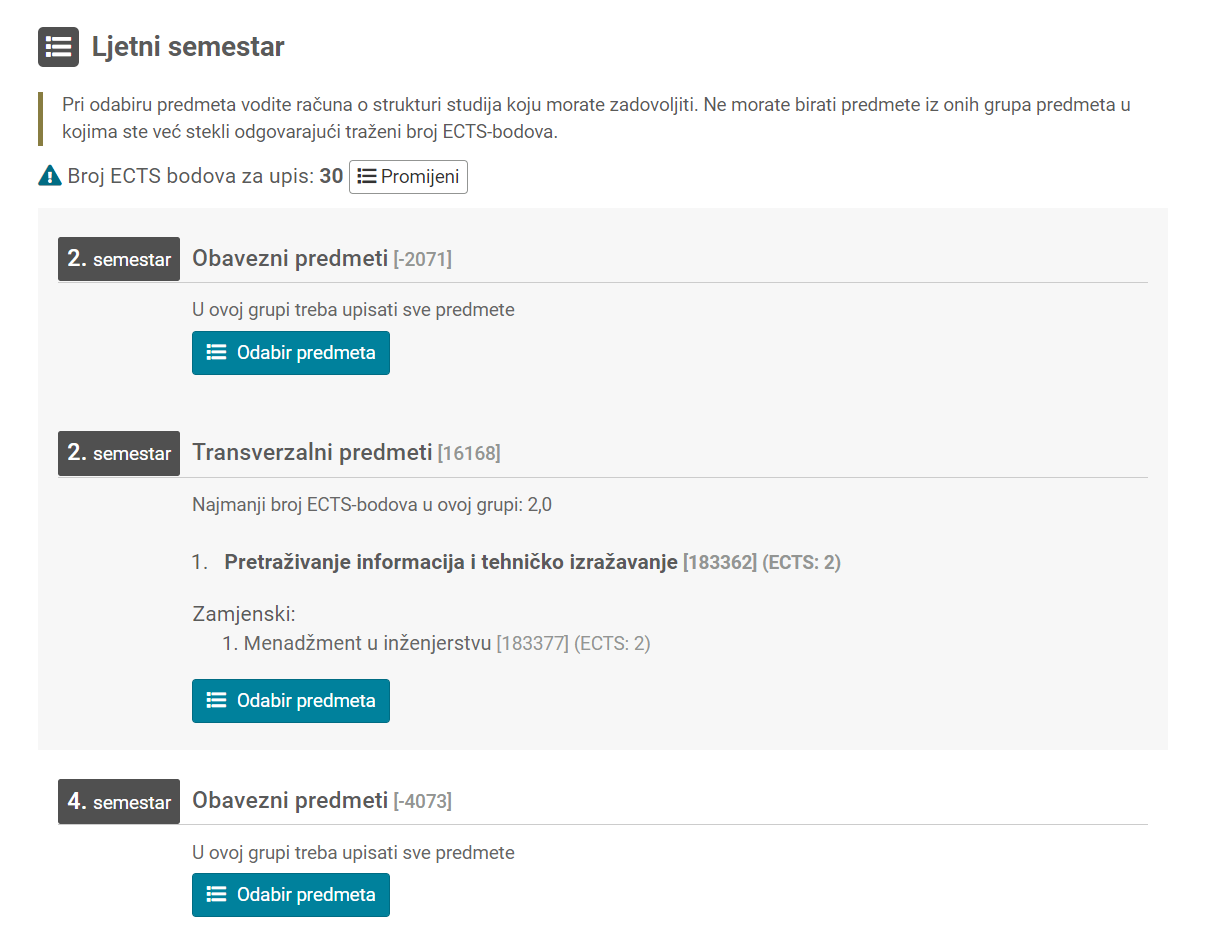
\includegraphics[scale=.45]{poboljsana/courses.png}}
      \centering
      \caption{Prikaz odabira semestara aplikacije poboljšanog dizajna}
    \end{figure}
    
    \begin{figure} [H]
      \fbox{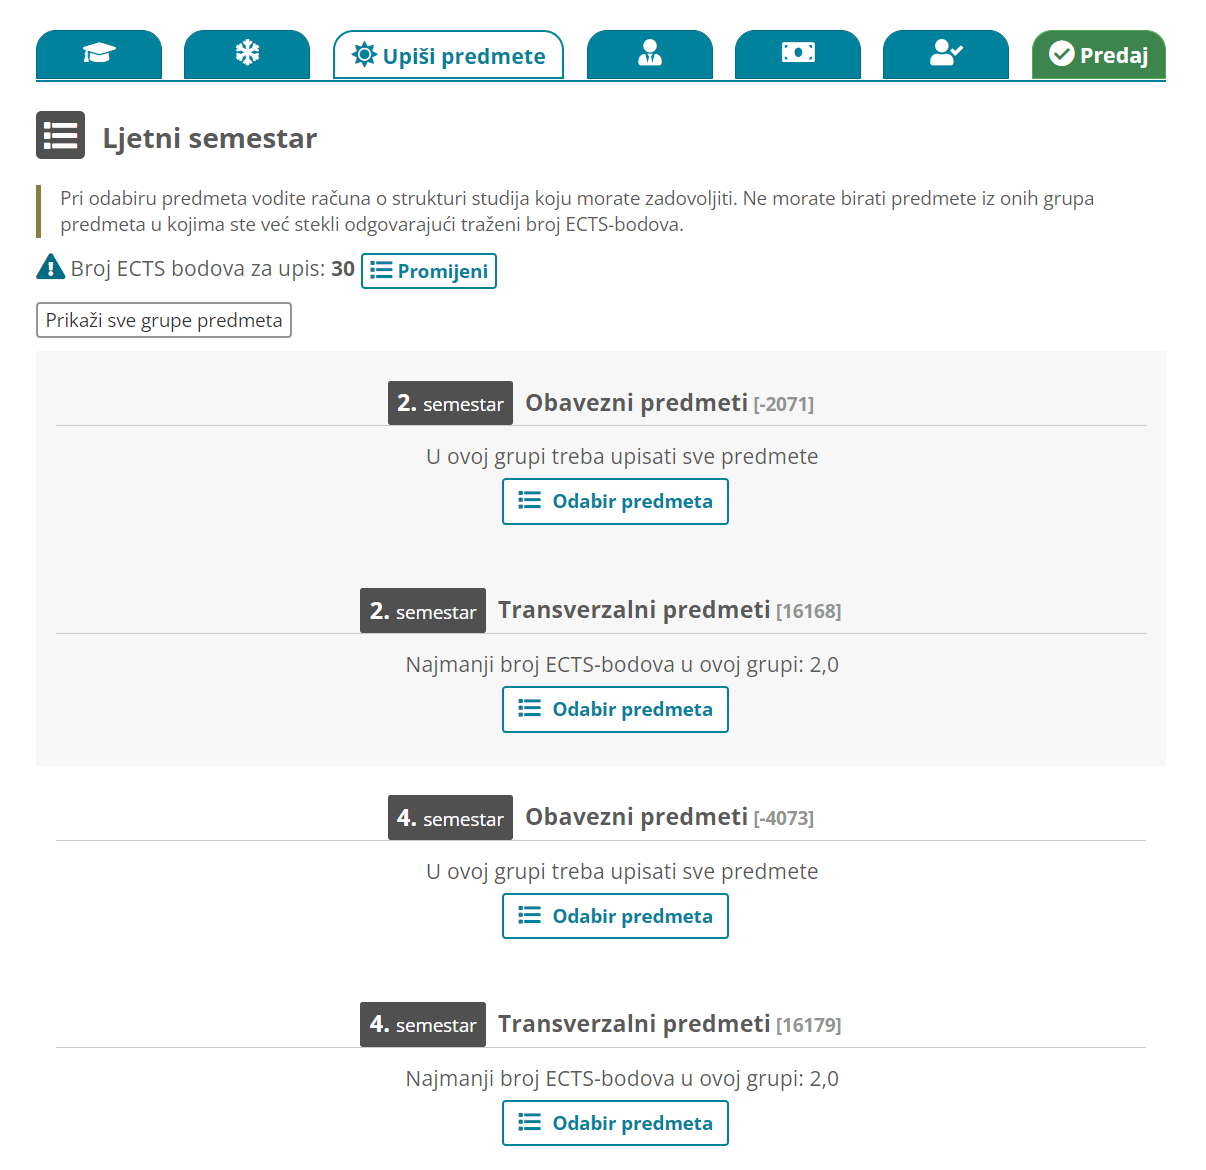
\includegraphics[scale=.45]{nova/courses_1.png}}
      \fbox{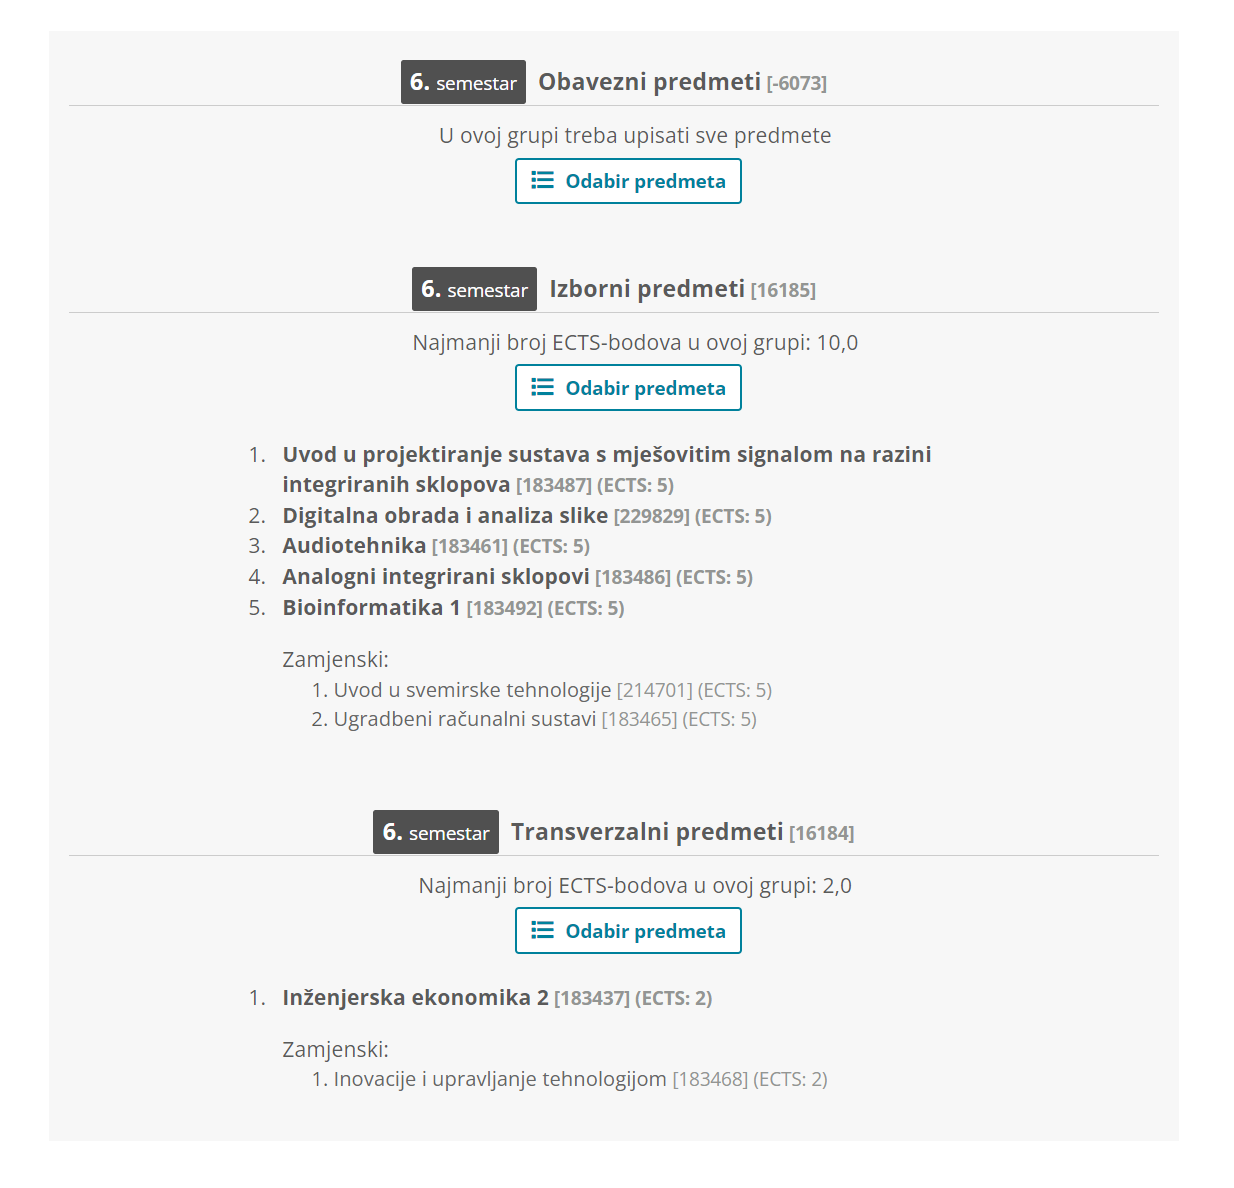
\includegraphics[scale=.45]{nova/courses_2.png}}
      \centering
      \caption{Prikaz odabira semestara aplikacije novog dizajna}
    \end{figure}
    
    
    Najveća promjena u izgledu stranice odabira predmeta dvaju novih dizajna s obzirom na stari je promjena pozicije gumba kod odabranih i zamjenskih predmeta. Gumbi su također pojednostavljeni uklanjanjem teksta. Kako su jednaki gumbi na takvom dizajnu pozicionirani jedan ispod drugog, student više ne mora tražiti gdje se nalaze pri svakom mijenjaju redoslijeda predmeta. U ovu svrhu dodana je i animacija pri zamjeni redoslijeda kao korisna povratna informacija da je korisnikova akcija obavljena. Iz istog razloga, animacija je dodana i pri dodavanju predmeta na liste.
    
    Uz to, implementirana je mogućnost prebacivanja predmeta iz odabranih izravno u zamjenske i obratno. Na starom dizajnu za istu akciju potrebno je ukloniti predmet s popisa, ponovno ga pronaći u listi dostupnih predmeta i onda ga dodati na željenu listu.
    
    Posljednja bitnija promjena na oba dizajna bila je dodavanje info-oblačića pri akciji \textit{hover} na oznake \textit{Ograničenje}, \textit{Ne održava se} i \textit{Nije moguće upisati}.
    
    Na novom dizajnu uz navedene promjene implementirano je i polje za pretraživanje čime korisnici ne moraju listati po dugačkom popisu dostupnih predmeta, već ga mogu pretražiti u polju po hrvatskom i engleskom nazivu ili ID-u.
    
    Navedenim promjenama poboljšana je funkcionalnost, a time i zadovoljstvo korisnika. Promjene su vidljive na slikama ispod.
    
    \begin{figure} [H]
      \fbox{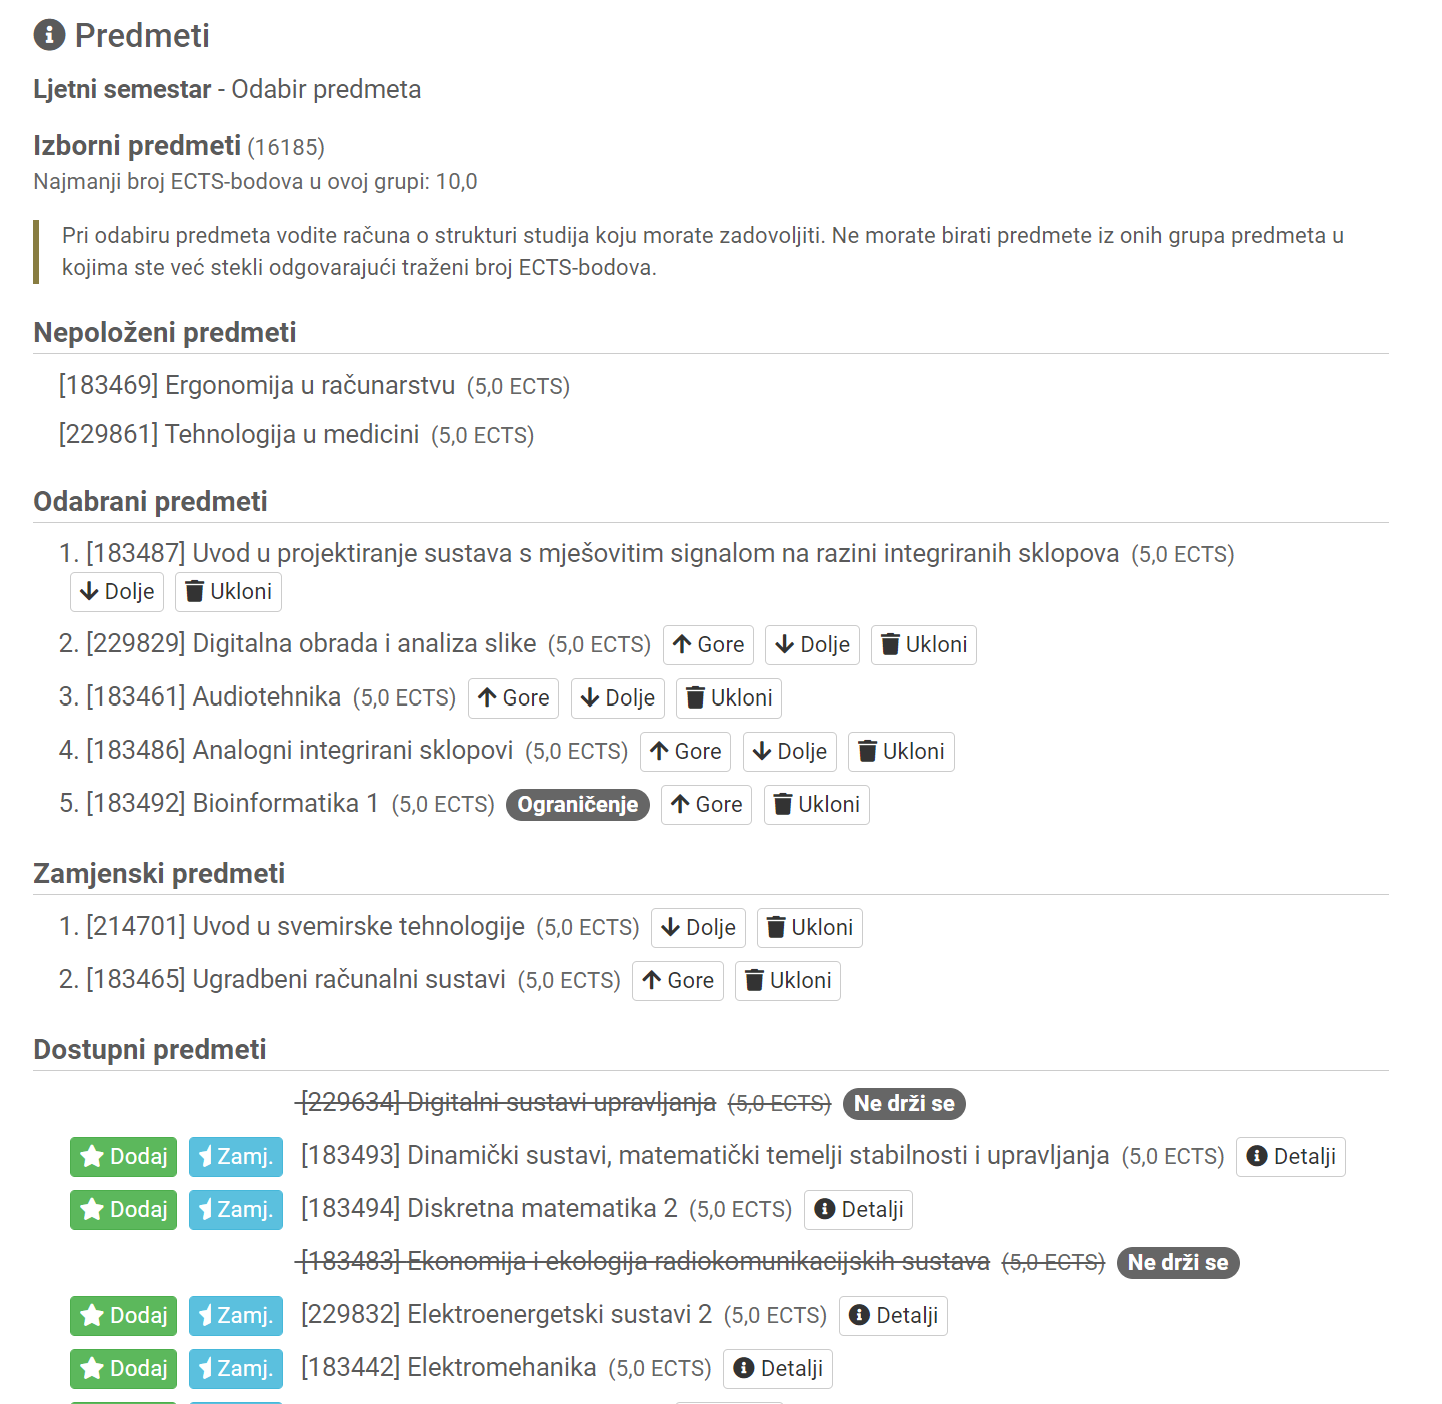
\includegraphics[scale=.5]{stara/selectcourses.png}}
      \centering
      \caption{Prikaz odabira predmeta aplikacije starog dizajna}
    \end{figure}
    
    \begin{figure} [H]
      \fbox{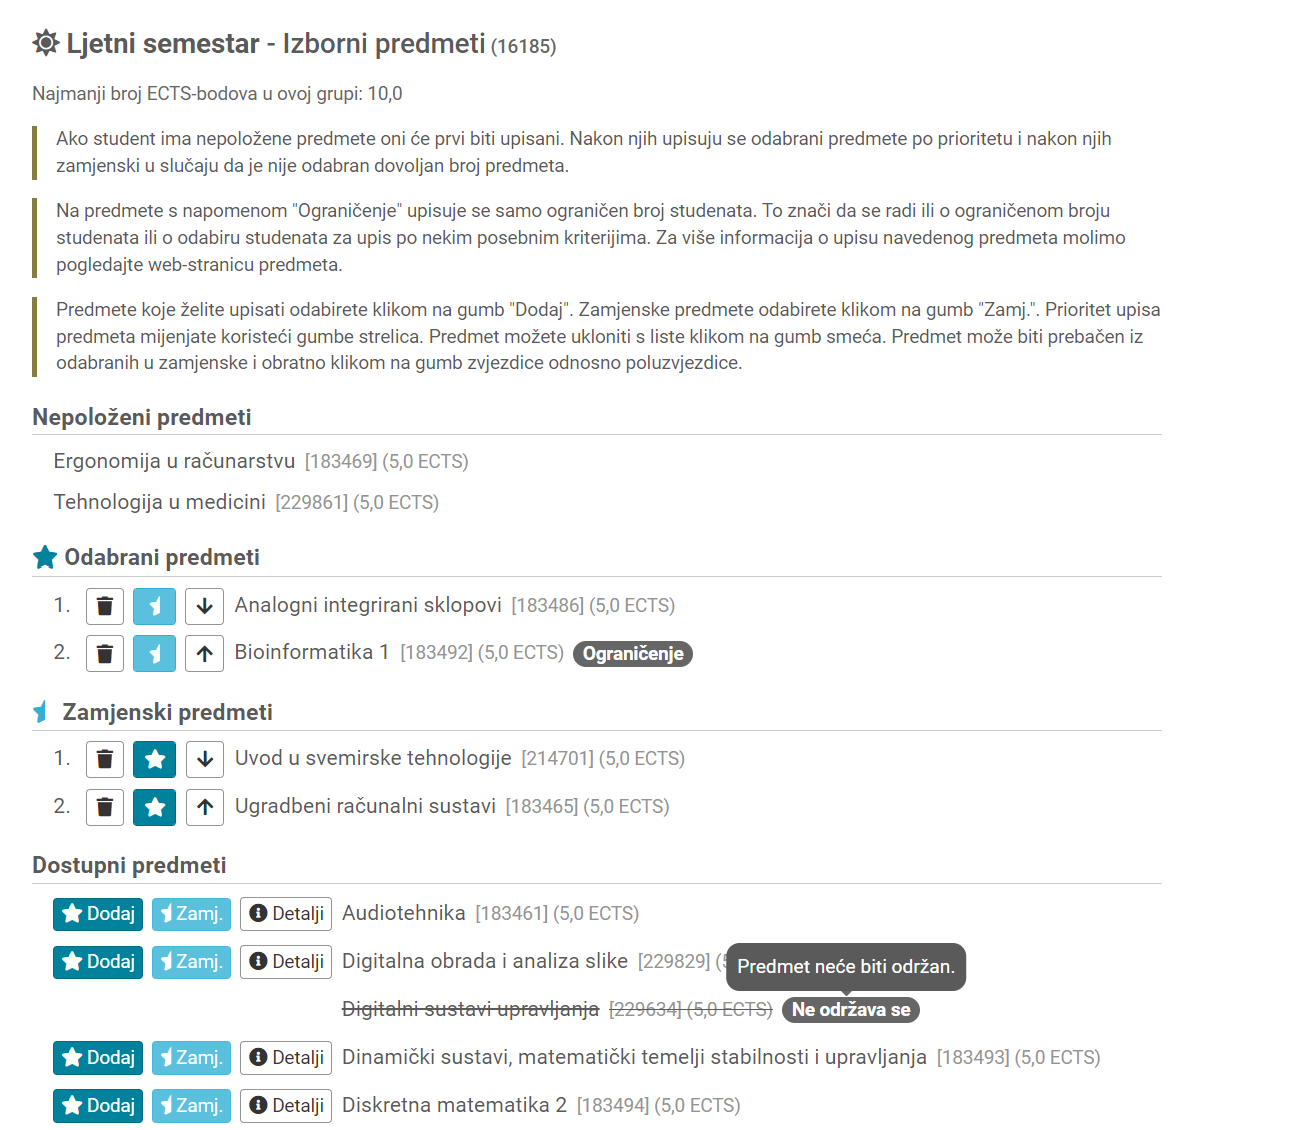
\includegraphics[scale=.5]{poboljsana/selectcourses.png}}
      \centering
      \caption{Prikaz odabira predmeta aplikacije poboljšanog dizajna}
    \end{figure}
    
    \begin{figure} [H]
      \fbox{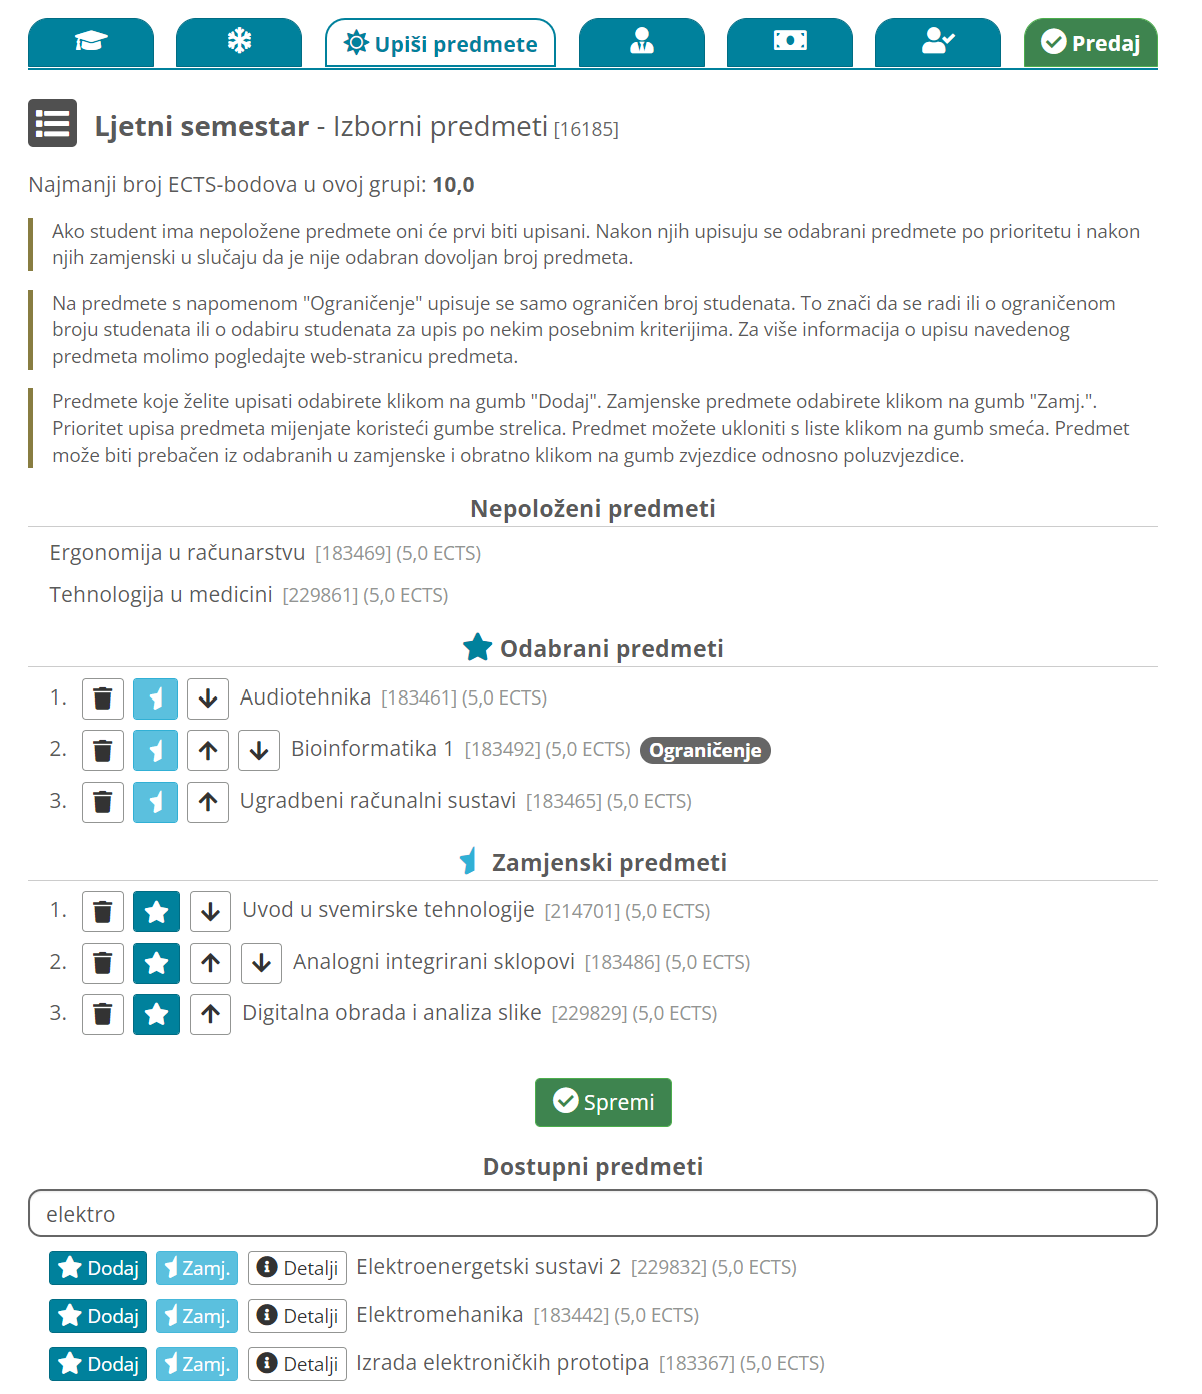
\includegraphics[scale=.5]{nova/selectcourses.png}}
      \centering
      \caption{Prikaz odabira predmeta aplikacije novog dizajna}
    \end{figure}
    
    Ocijenjeno iskustvo korištenja ovih stranica je poraslo s \textbf{3.8} na \textbf{4.2} za poboljšani dizajn i kasnije na \textbf{4.4} za novi dizajn.
    
    \vspace{\baselineskip}
    \bigbreak
    \bigbreak
    \noindent\textbf{Plaćanje}
    
    Na stranici plaćanja u poboljšanom dizajnu tablica računa je proširena i centrirana. Time je preglednost tablice povećana. Izgled nije puno promijenjen i to je vidljivo iz ocjena iz evaluacije za ovu stranicu. Na novom dizajnu stranice uklonjen je sav tekst iznad tablice osim \textit{Ukupno za platiti:} i podebljanog iznosa dûga u kunama. Na tablicu je dodan obrub i njezini retci se više ne stapaju s pozadinom. Tablica je još više proširena i tekst u njoj centriran kako bi bila što preglednija. Zbog načina pohrane podataka u bazu koju aplikacija koristi, nije moguće učiniti dizajn potpuno jasnim za korisnika. Ispod tablice dodano je kratko objašnjenje redaka u tablici kako bi se što više smanjila zbunjenost studenata.
    
    Sva tri dizajna prikazana su na slikama:
    
    \begin{figure} [H]
      \fbox{\includegraphics[scale=.45]{stara/payment.png}}
      \centering
      \caption{Prikaz plaćanja aplikacije starog dizajna}
    \end{figure}
    
    \begin{figure} [H]
      \fbox{\includegraphics[scale=.5]{poboljsana/payment.png}}
      \centering
      \caption{Prikaz plaćanja aplikacije poboljšanog dizajna}
    \end{figure}
    
    \begin{figure} [H]
      \fbox{\includegraphics[scale=.5]{nova/placanje.png}}
      \centering
      \caption{Prikaz plaćanja aplikacije novog dizajna}
    \end{figure}
    
    Ocjena dobivena evaluacijom dizajna za iskustvo studenata sa stranicom plaćanja porasla je s \textbf{1.8}, za stari dizajn, na \textbf{2} za poboljšani. Ovo nije velika razlika što je jasno s obzirom na količinu promjena u dizajnu. Međutim, prosječna ocjena za novi dizajn porasla je na \textbf{3.8}. Ovo pokazuje kako korisnici mogu imati dobro iskustvo s aplikacijama s kojima komuniciraju iako njihova funkcionalnost nije zadovoljavajuća.
    
    Uz ove, posebno istaknute stranice, mijenjao se izgled i ostalih kako bi bolje odgovarao ciljanoj skupini korisnika. Prosječna ocjena za ukupno iskustvo s aplikacijom starog dizajna bila je \textbf{3.2}. Ona je porasla na \textbf{4} kod poboljšanog dizajna. Na kraju, za aplikaciju novog dizajna prosječna ocjena dobivena evaluacijom iznosila je \textbf{4.2}. Iz usporedbe ovih rezultata vidi se kako su obavljene promjene u dizajnu poboljšale iskustvo korištenja aplikacije.

     
    
    


\chapter{Zaključak}

%Zaključak koji ste napisali nije sažetak, recimo da je "dobro", tj. dobar je taj put. Malo su mi čudne/nerazumljive neke izjave, ajde probajte budne glave to još malo raspisati, što je pisac htio reći, i što iz svega ovoga zaključujete. I nemojte u tom procesu pretvoriti Zaključak u Sažetak


S količinom web-aplikacija i korisničkih sučelja u današnje doba, nije više dovoljno da sučelje bude samo funkcionalno. Minimalni kriteriji koje bi danas svaka aplikacija trebala zadovoljiti su viši nego prije i samo će nastaviti rasti s vremenom. Svaka aplikacija rađena je s određenim ciljem i za određenu grupu korisnika. S obzirom na ciljanu grupu, bila to dob korisnika ili njihovo zanimanje, osobe koje rade dizajn i razvijaju aplikacije trebaju imati na umu kakve karakteristike ima grupa.
%S obzirom na karakteristike, aplikacija treba biti prilagođena upravo tim korisnicima. Nema smisla razviti šarenu aplikaciju po kojoj kretanje i razumijevanje opcija ovisi isključivo o boji ako je aplikacija rađena za ljude s daltonizmom ili imati tekst malih slova ako radimo aplikaciju pretežno za ljude starije dobi.

Korisnike primarno privlači atraktivan i upečatljiv izgled web-stranica i aplikacija. Iskustvo pokazuje da su korisnici skloni oprostiti neke funkcijske nedostatke ili manje poteškoće ako se u njima izaziva pozitivna emocija ili barem ne izaziva neka negativna. Ovo se najlakše ostvaruje vizualnim putem. Isto je vidljivo iz rezultata evaluacija. Struktura stranice za plaćanje i stranice za odabir semestra ostala je jednaka. Promijenjen je isključivo prikaz te strukture. Manje promjene u dizajnu mogu jako djelovati na iskustvo korisnika.

Na stranici biranja predmeta za upis atraktivan izgled ne bi bio dovoljan da korisnik bude zadovoljan. Ovdje postaje bitan pokretni dizajn u sučelju korišten na ispravan način kako bi korisniku dao povratnu informaciju o njegovim
akcijama i time povećao njegovo zadovoljstvo korištenja.



\nocite{*}
\bibliography{literatura}
\bibliographystyle{unsrt}

\begin{sazetak}
%Sažetak na hrvatskom jeziku.
%Dizajn je važan, na više načina, pokretni dizajn može pomoći u funkcionalnosti. Ovo je pokazano na primjeru toga i toga, gdje je u radu evaluiran postojeći dizajn. Temeljem rezultata razvijena je poboljšana verzija, .... ali ne samo to, razvijen je i drugačiji dizajn, više oslonjen na pokretni dizajn. Evalucija je pokazala blabla. Kraj." 

Osim funkcionalnosti web-aplikacija, bitan je i njihov dizajn. Atraktivan dizajn pridonosi korisničkom iskustvu. Uz njega, suptilne animacije korisniku jasnije daju povratnu informaciju nego statički dizajn. Kao primjer važnosti dizajna, uzet je postojeći modul sustava QuiltCMS za upis akademske godine na Fakultetu elektrotehnike i računarstva. O korisničkom iskustvu uporabe modula provedeno je kratko istraživanje sa studentima. Na temelju njihovih komentara i dobrih praksi izrade korisničkih sučelja osmišljen je i implementiran poboljšani dizajn modula. Uz evaluaciju poboljšanog dizajna modula, osmišljen je, izrađen i evaluiran novi dizajn, koji se temelji na pokretnom dizajnu. Pri svakoj evaluaciji, studenti su ocjenjivali svoje iskustvo korištenja određenih stranica i iskustvo korištenja cijele aplikacije. Ovi rezultati su uspoređeni i komentirani. Svakom novom promjenom dizajna, temeljenom na povratnim informacijama korisnika, dane ocjene za iskustvo korištenja su rasle. Ovim radom pokazan je značaj izrade sučelja s korisnikom u prvom planu i prednosti korištenja pokretnog dizajna kao elementa korisničkog sučelja.



\kljucnerijeci{pristupačnost, korisničko sučelje, UI, korisničko iskustvo, UX, pokretni dizajn}
\end{sazetak}

% TODO: Navedite naslov na engleskom jeziku.
\vspace{\baselineskip}
\bigbreak
\engtitle{Adaptation of web application user interfaces to motion design concepts}
\begin{abstract}
%Abstract.
In addition to the functionality of web applications, their design is also important. Attractive design contributes to the user experience. Along with it, subtle animations give the user clearer feedback than static design. As an example of the importance of design, the existing module of the QuiltCMS system for enrollment in the academic year at the Faculty of Electrical Engineering and Computing was taken. A short research with students was conducted on the user experience of using the module. Based on their comments and good user interface design practices, an improved module design was designed and implemented. In addition to the evaluation of the improved module design, a new design based on the motion design was designed, developed and evaluated. In each evaluation, students evaluated their experience of using specific pages and experience of using the entire application. These results were compared and commented on. With each new design change, based on user feedback, the ratings given for the usage experience grew. This paper shows the importance of creating a user interface with the user in the foreground and the advantages of using motion design as an element of the user interface.

\keywords{accessibility, user interface, UI, user experience, UX, motion design}
\end{abstract}

\end{document}
